\documentclass[../thesis.tex]{subfiles}

\begin{document}
\section{Application Architecture}

\subsection{Architectural Design}
\begin{figure}[H]
    \centering
    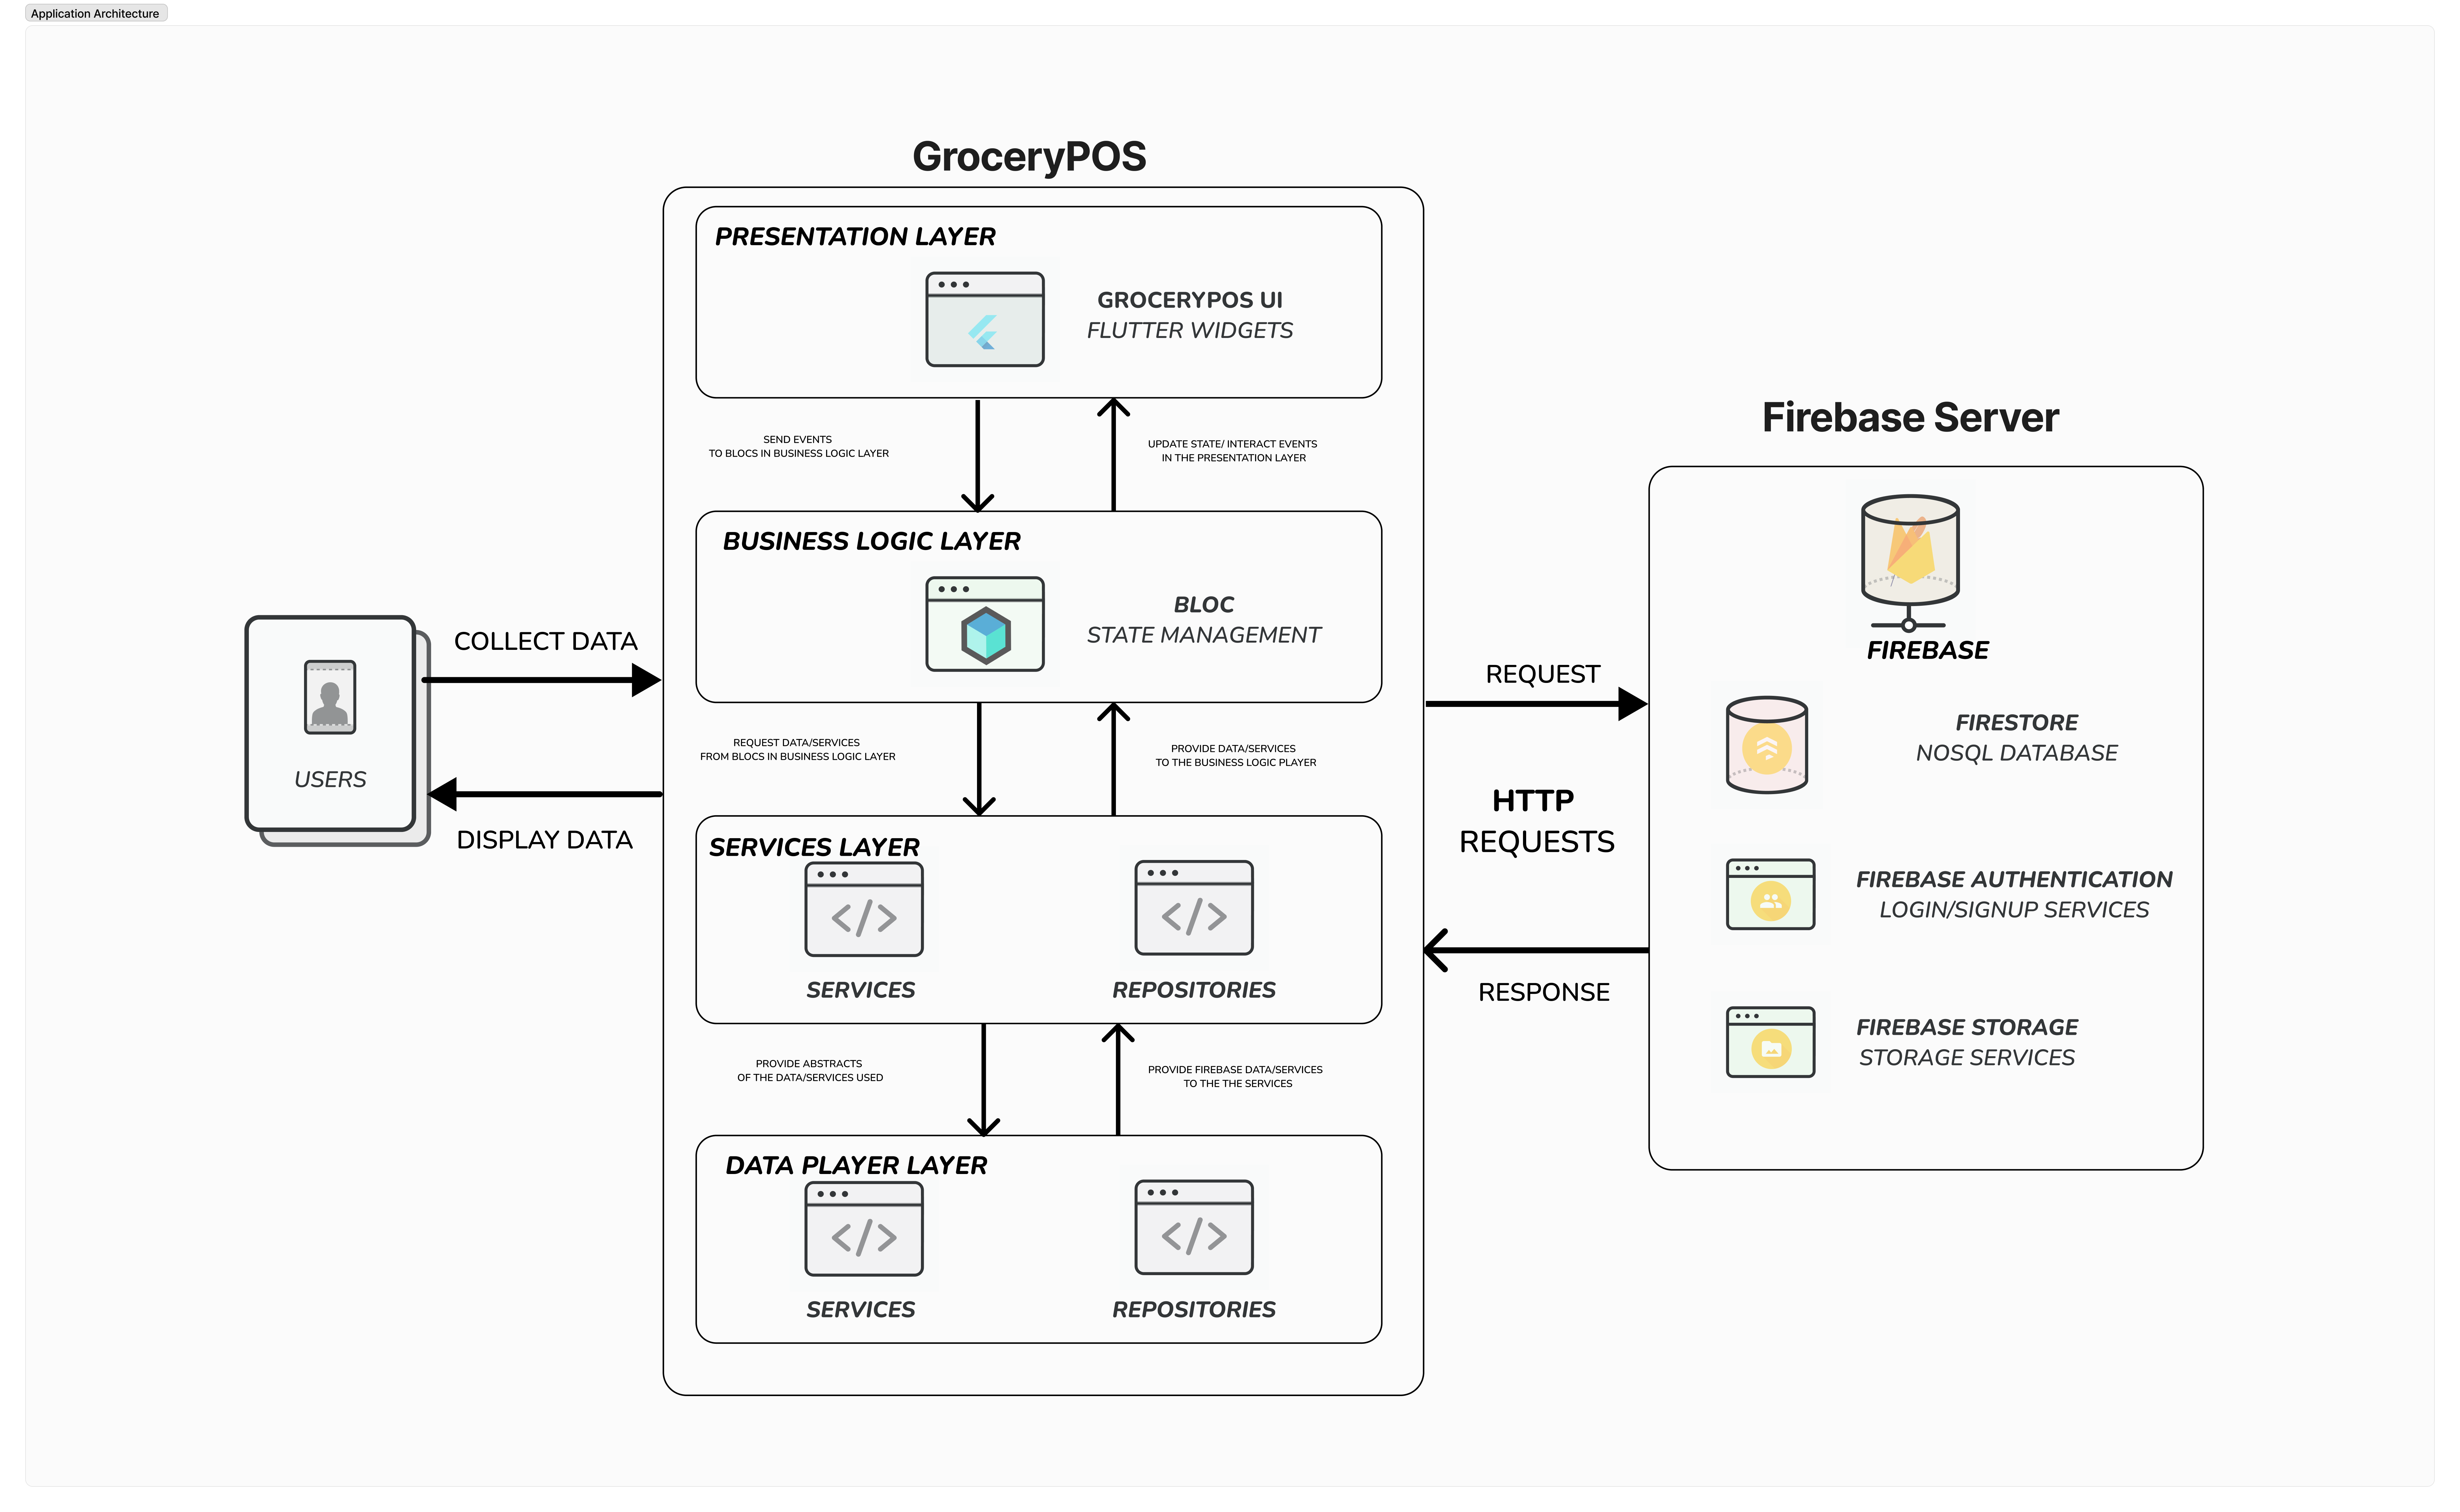
\includegraphics[width=1\textwidth]{images/Application-Architecture.png}
    \caption{Application Architecture}
    \label{fig:application-architecture}
\end{figure}
\subsection{Decomposition Description}
\begin{figure}[H]
    \centering
    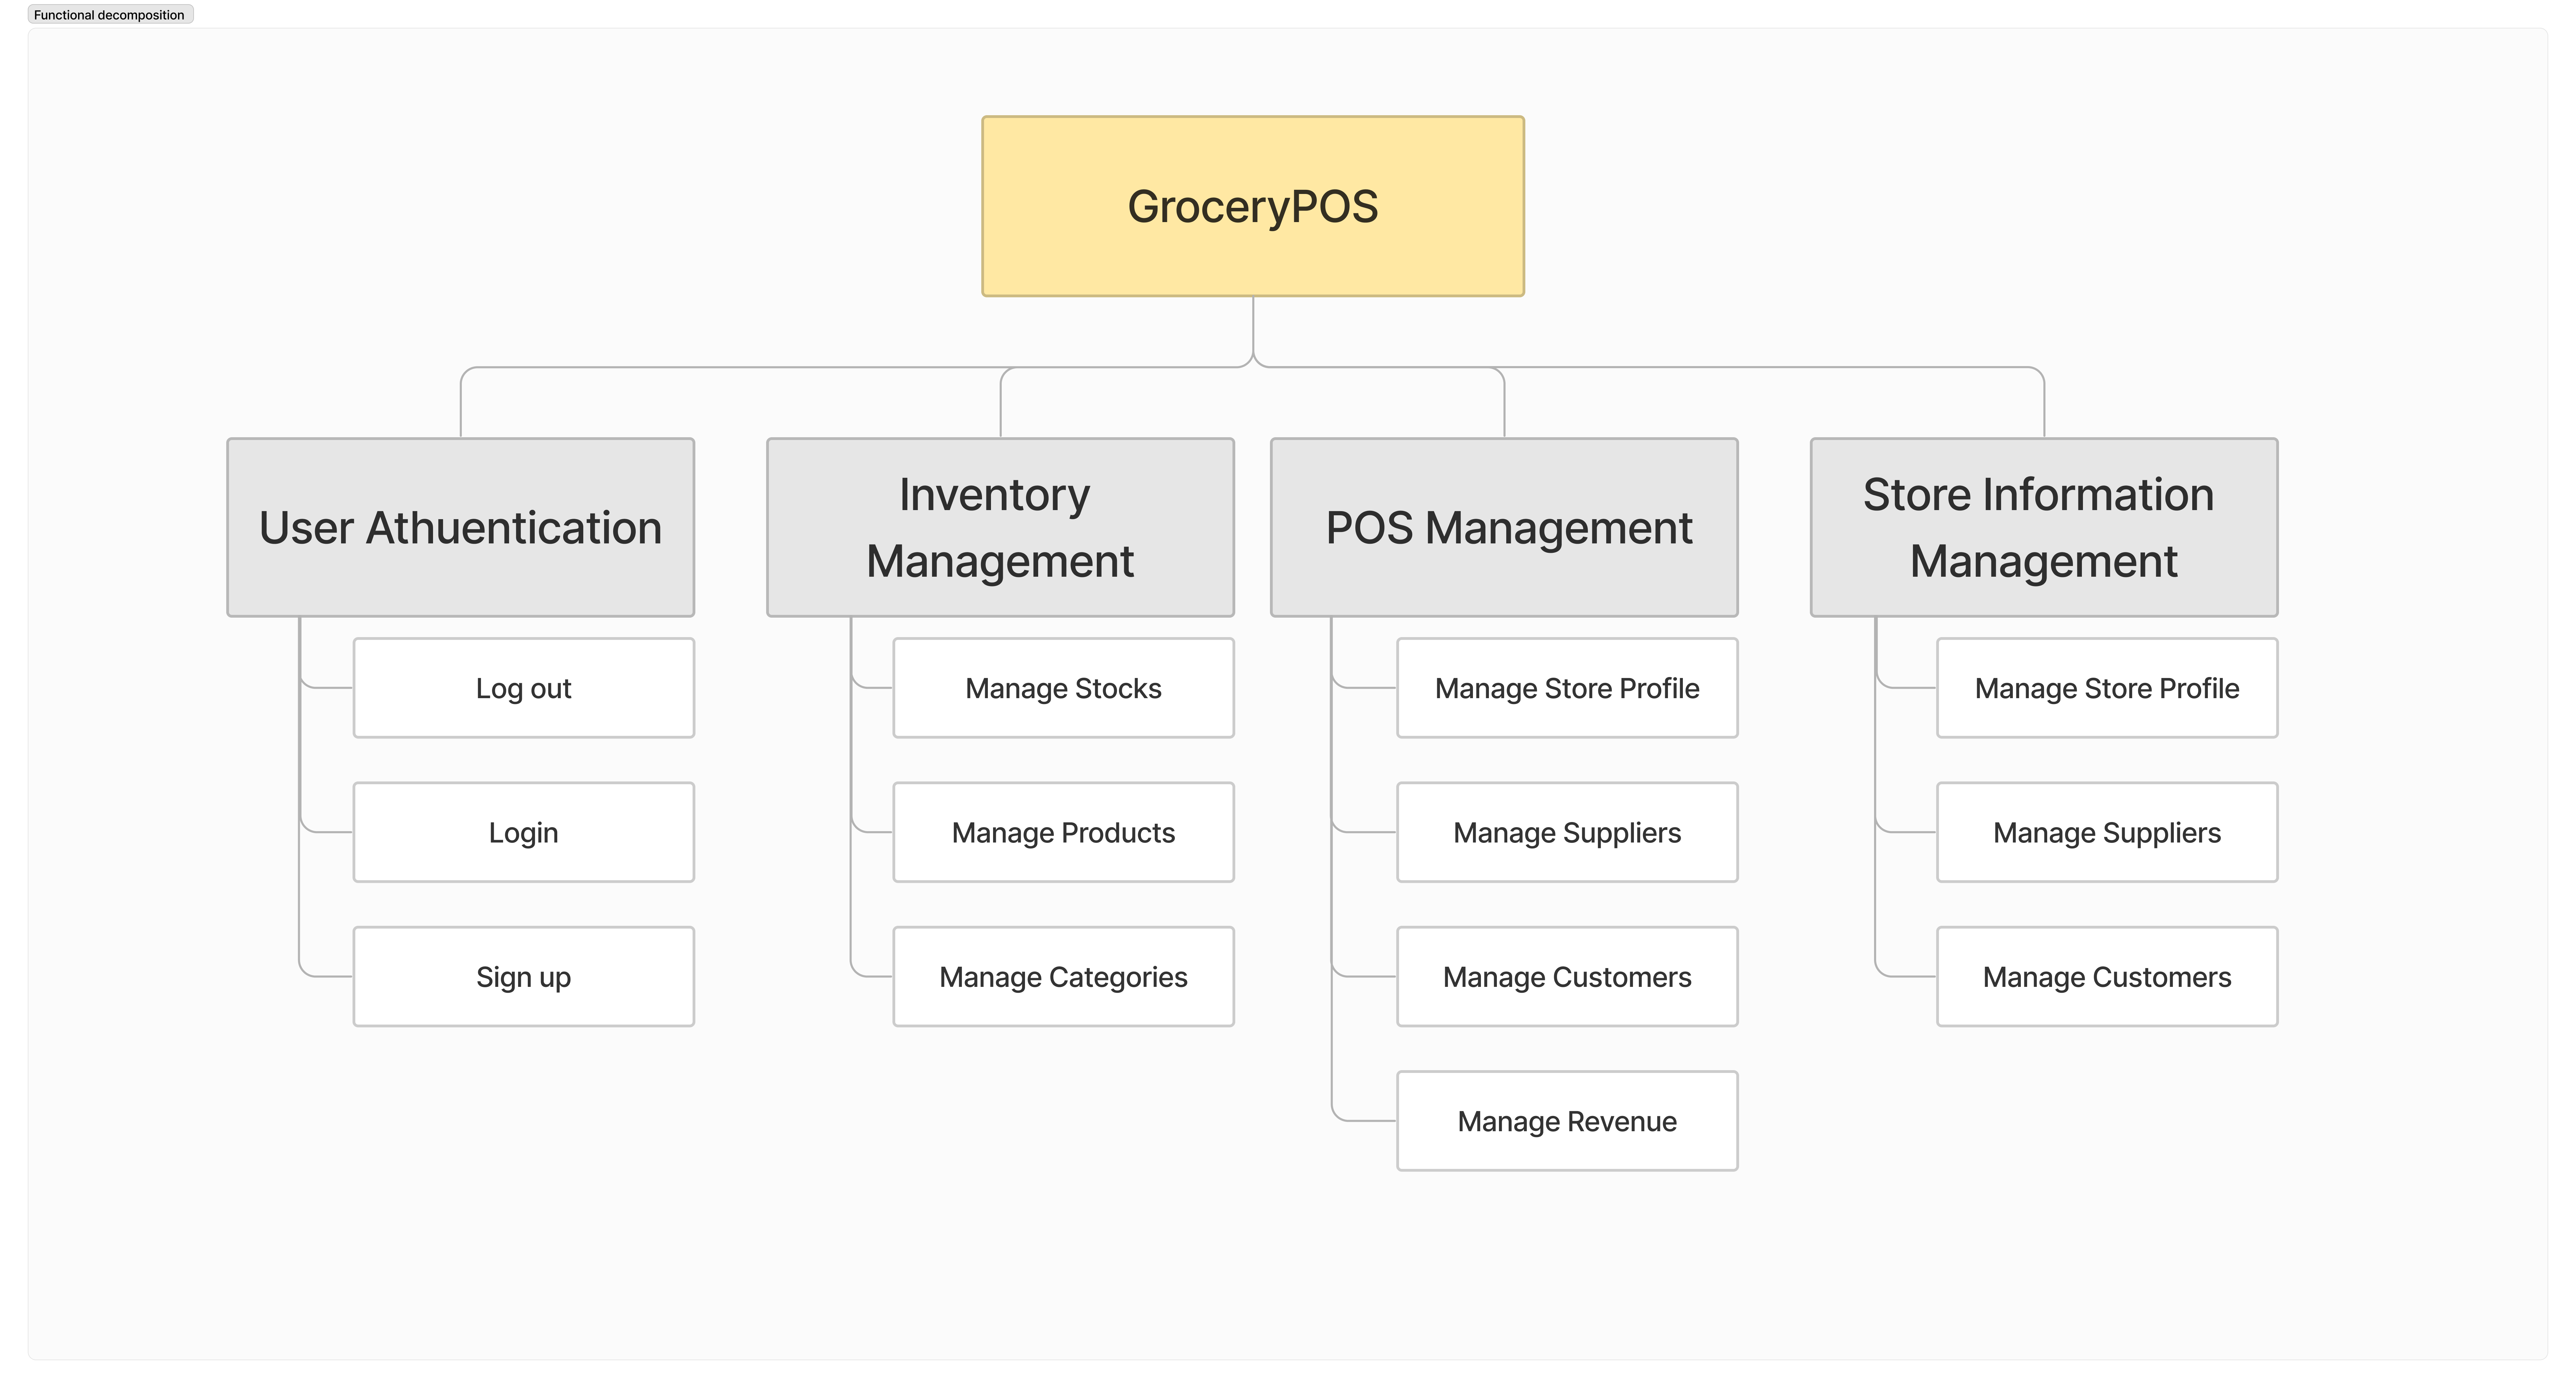
\includegraphics[width=1\textwidth]{images/Functional-Decomposition.png}
    \caption{Decomposition Description}
    \label{fig:functional-decomposition}
\end{figure}
% System
% |
% |-- User Authentication
% |   |-- Login
% |   |-- Logout
% |
% |-- Inventory Management
% |   |-- Inventory Tracking
% |   |-- Product Management
% |   |   |-- Add Product
% |   |   |-- Edit Product
% |   |   |-- Delete Product
% |   |
% |   |-- Category Management
% |
% |-- Sales Management
% |   |-- Invoice Creation
% |   |-- Invoice Management
% |   |   |-- View Invoice
% |   |   |-- Edit Invoice
% |   |   |-- Delete Invoice
% |   |
% |   |-- Invoice Printing
% |   |-- Revenue and Expenditure Management
% |
% |-- Store Information Management
%     |-- Supplier Management
%     |   |-- Add Supplier
%     |   |-- Edit Supplier
%     |   |-- Delete Supplier
%     |
%     |-- Customer Management
%         |-- Add Customer
%         |-- Edit Customer
%         |-- Delete Customer

% \subsection{Design Basis}
\section{Data Design}
\subsection{Data Description}
\subsubsection{Entity-Relationship Diagram}
\begin{figure}[H]
    \centering
    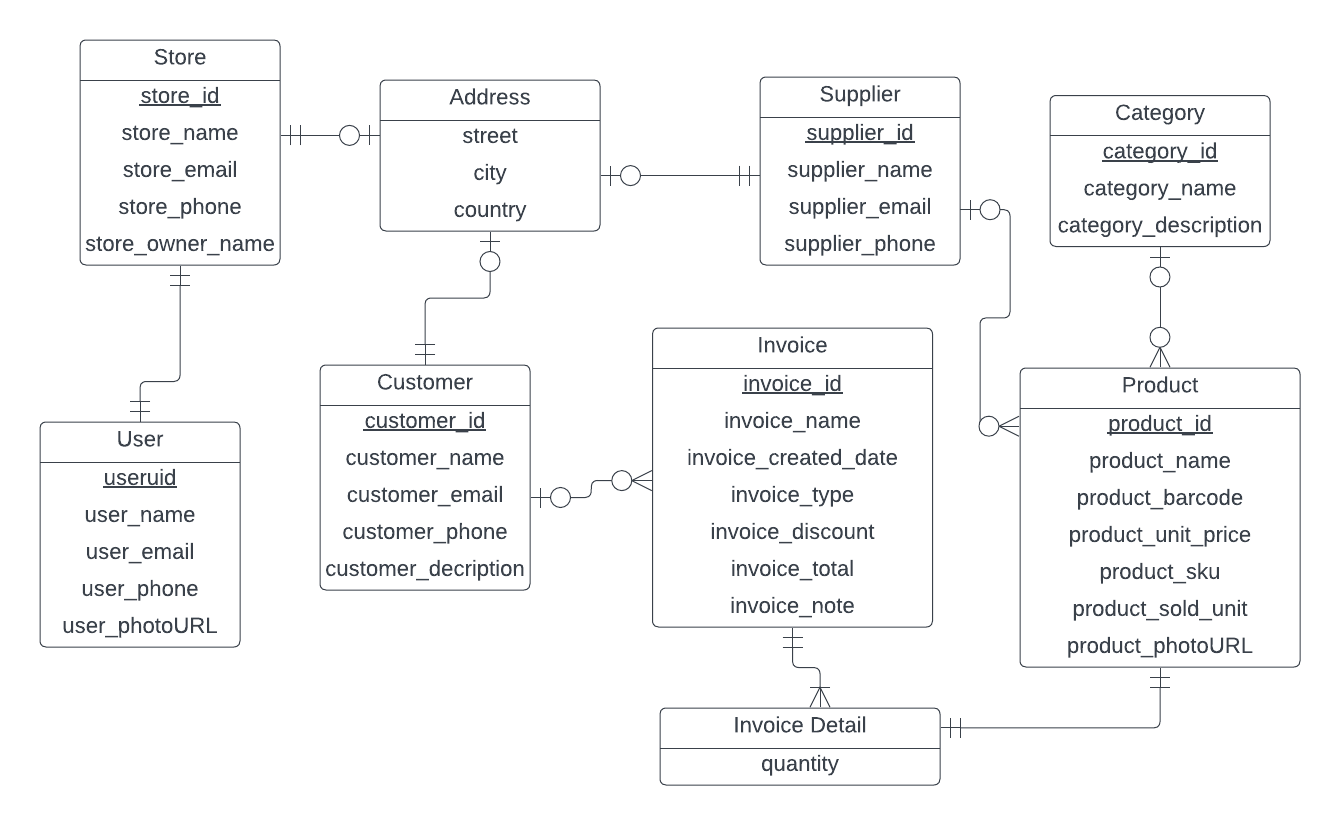
\includegraphics[width=0.75\textwidth]{images/ER_Diagram.png}
    \caption{Entity-Relationship Diagram}
    \label{fig:ER_Diagram}
\end{figure}
\subsubsection{Firebase Database Diagram}
\subsubsection*{The root of Firebase Firestore Database: }

\begin{figure}[H]
    \centering
    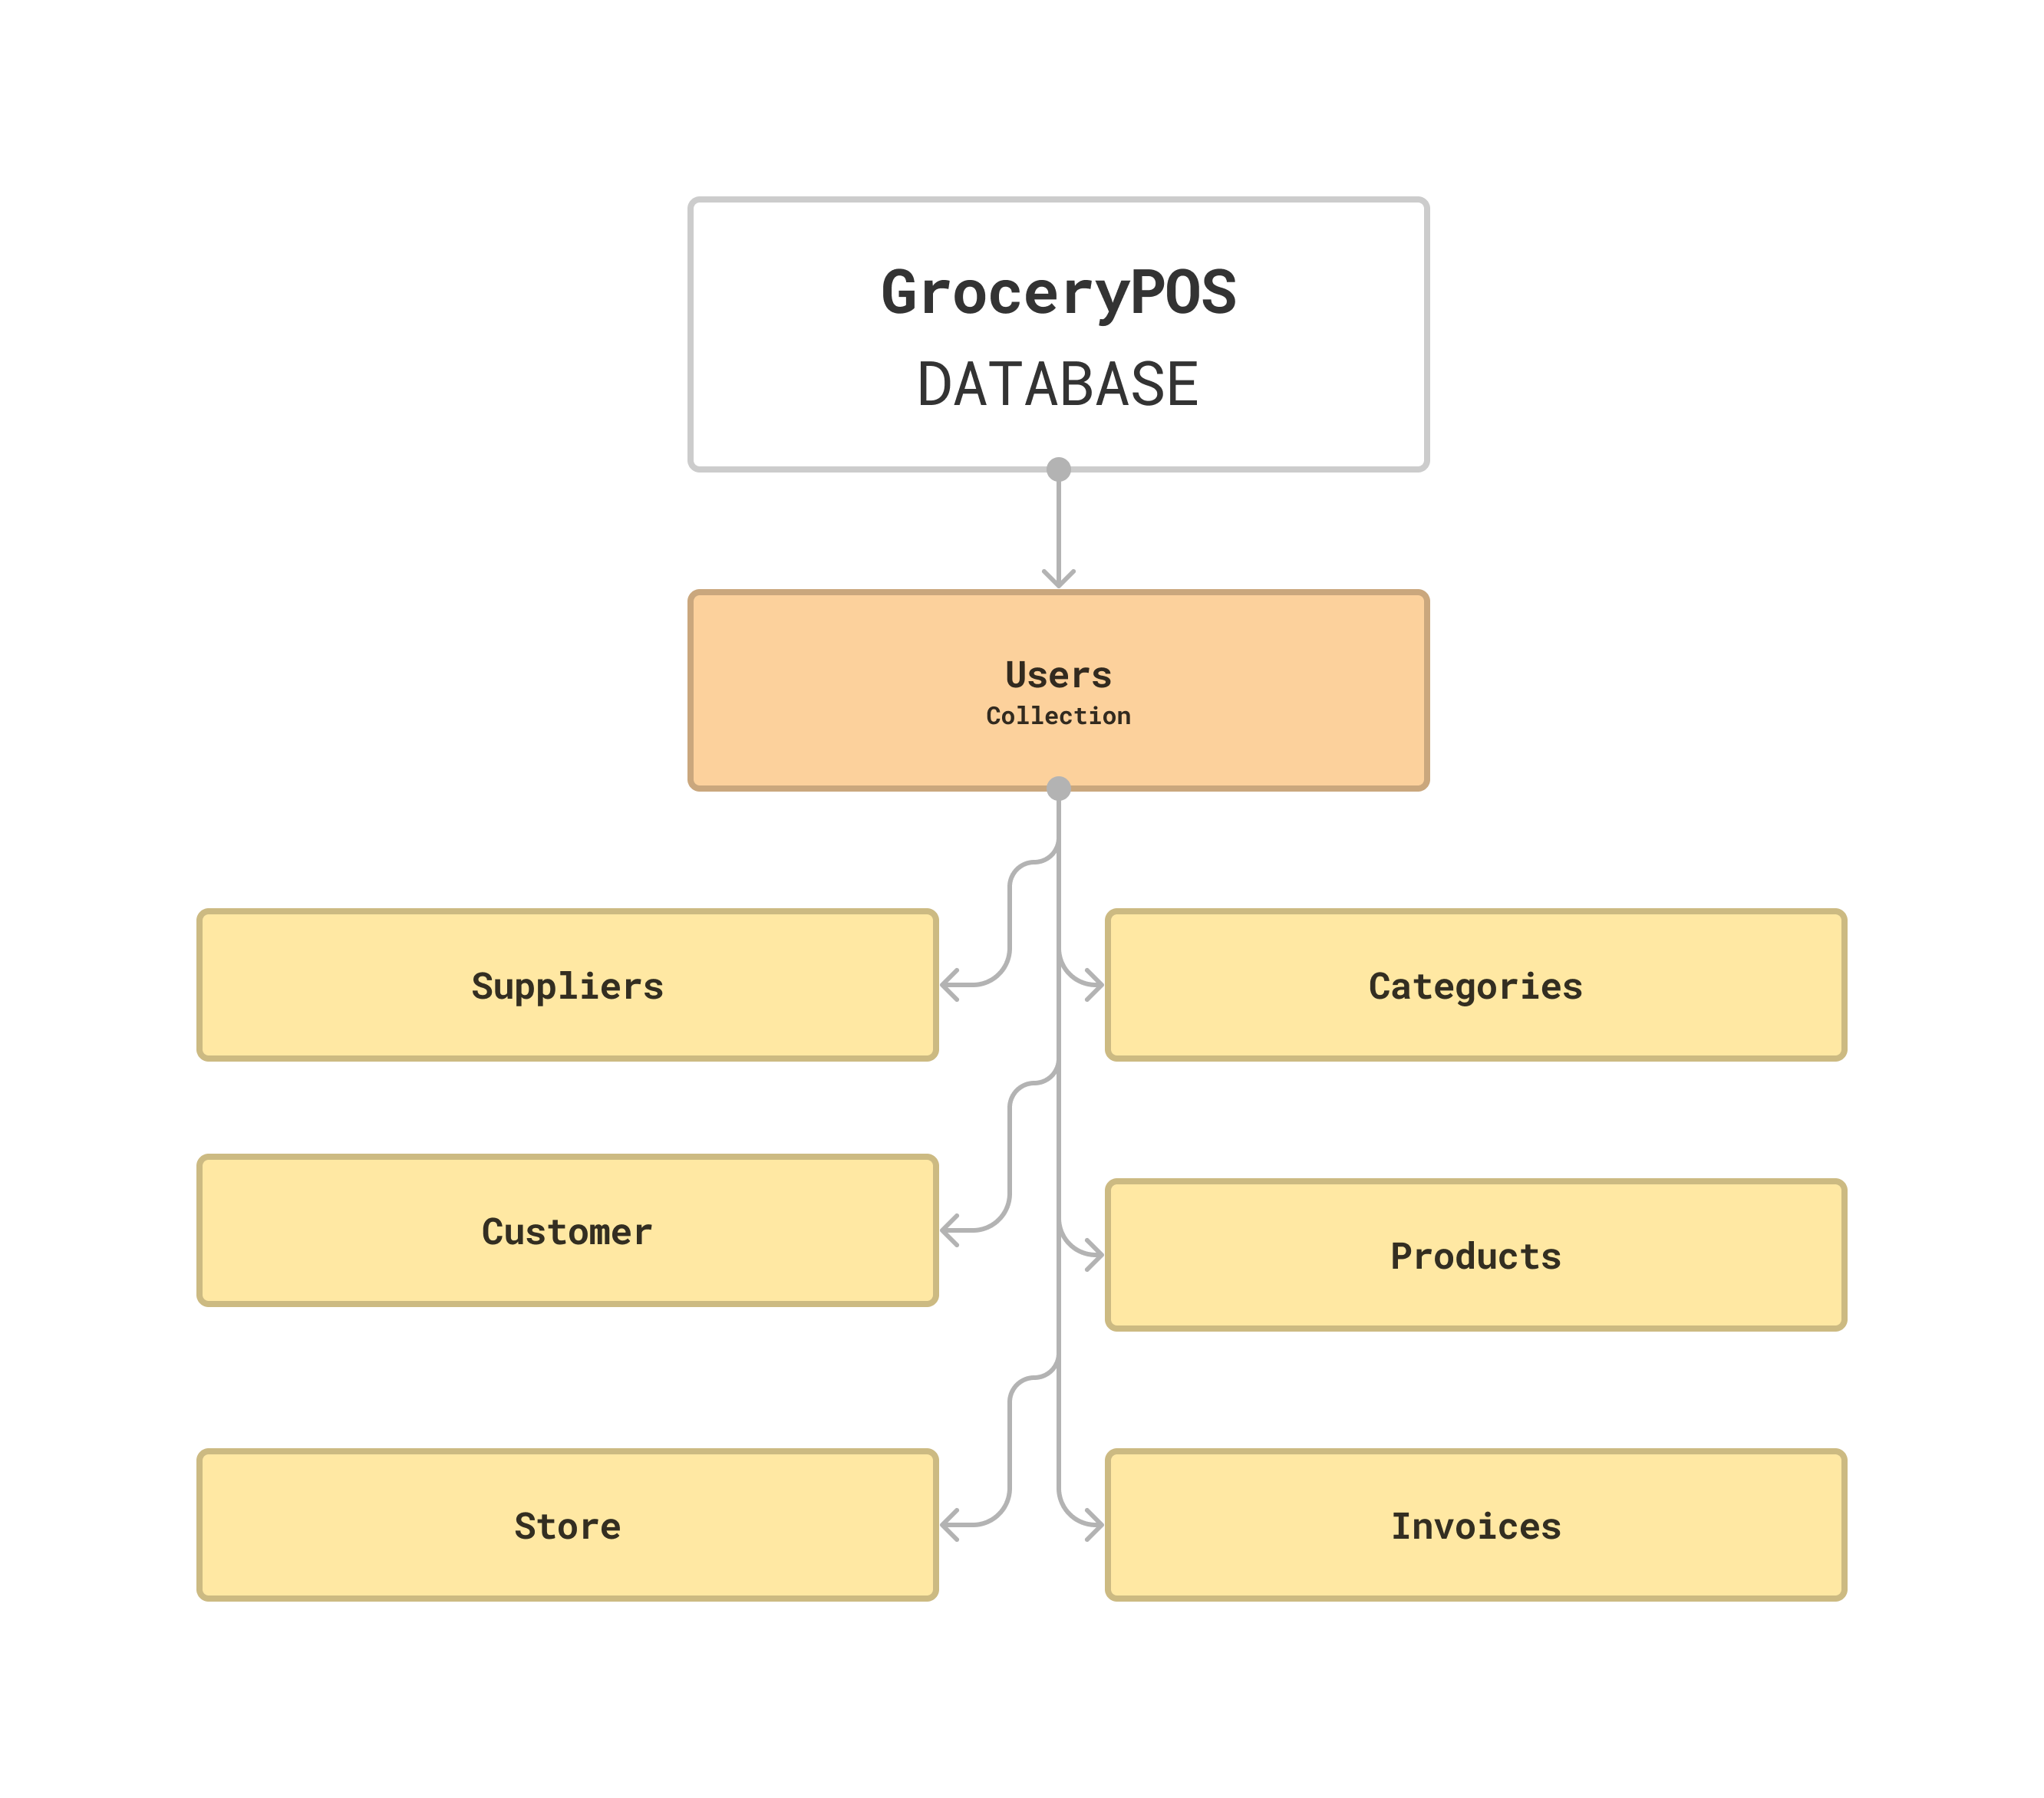
\includegraphics[width=0.9\textwidth]{images/Firebase_General.png}
    \caption{Firestore General}
    \label{fig:Firestore_General}
\end{figure}
\subsubsection*{The User collections:}

\begin{figure}[H]
    \centering
    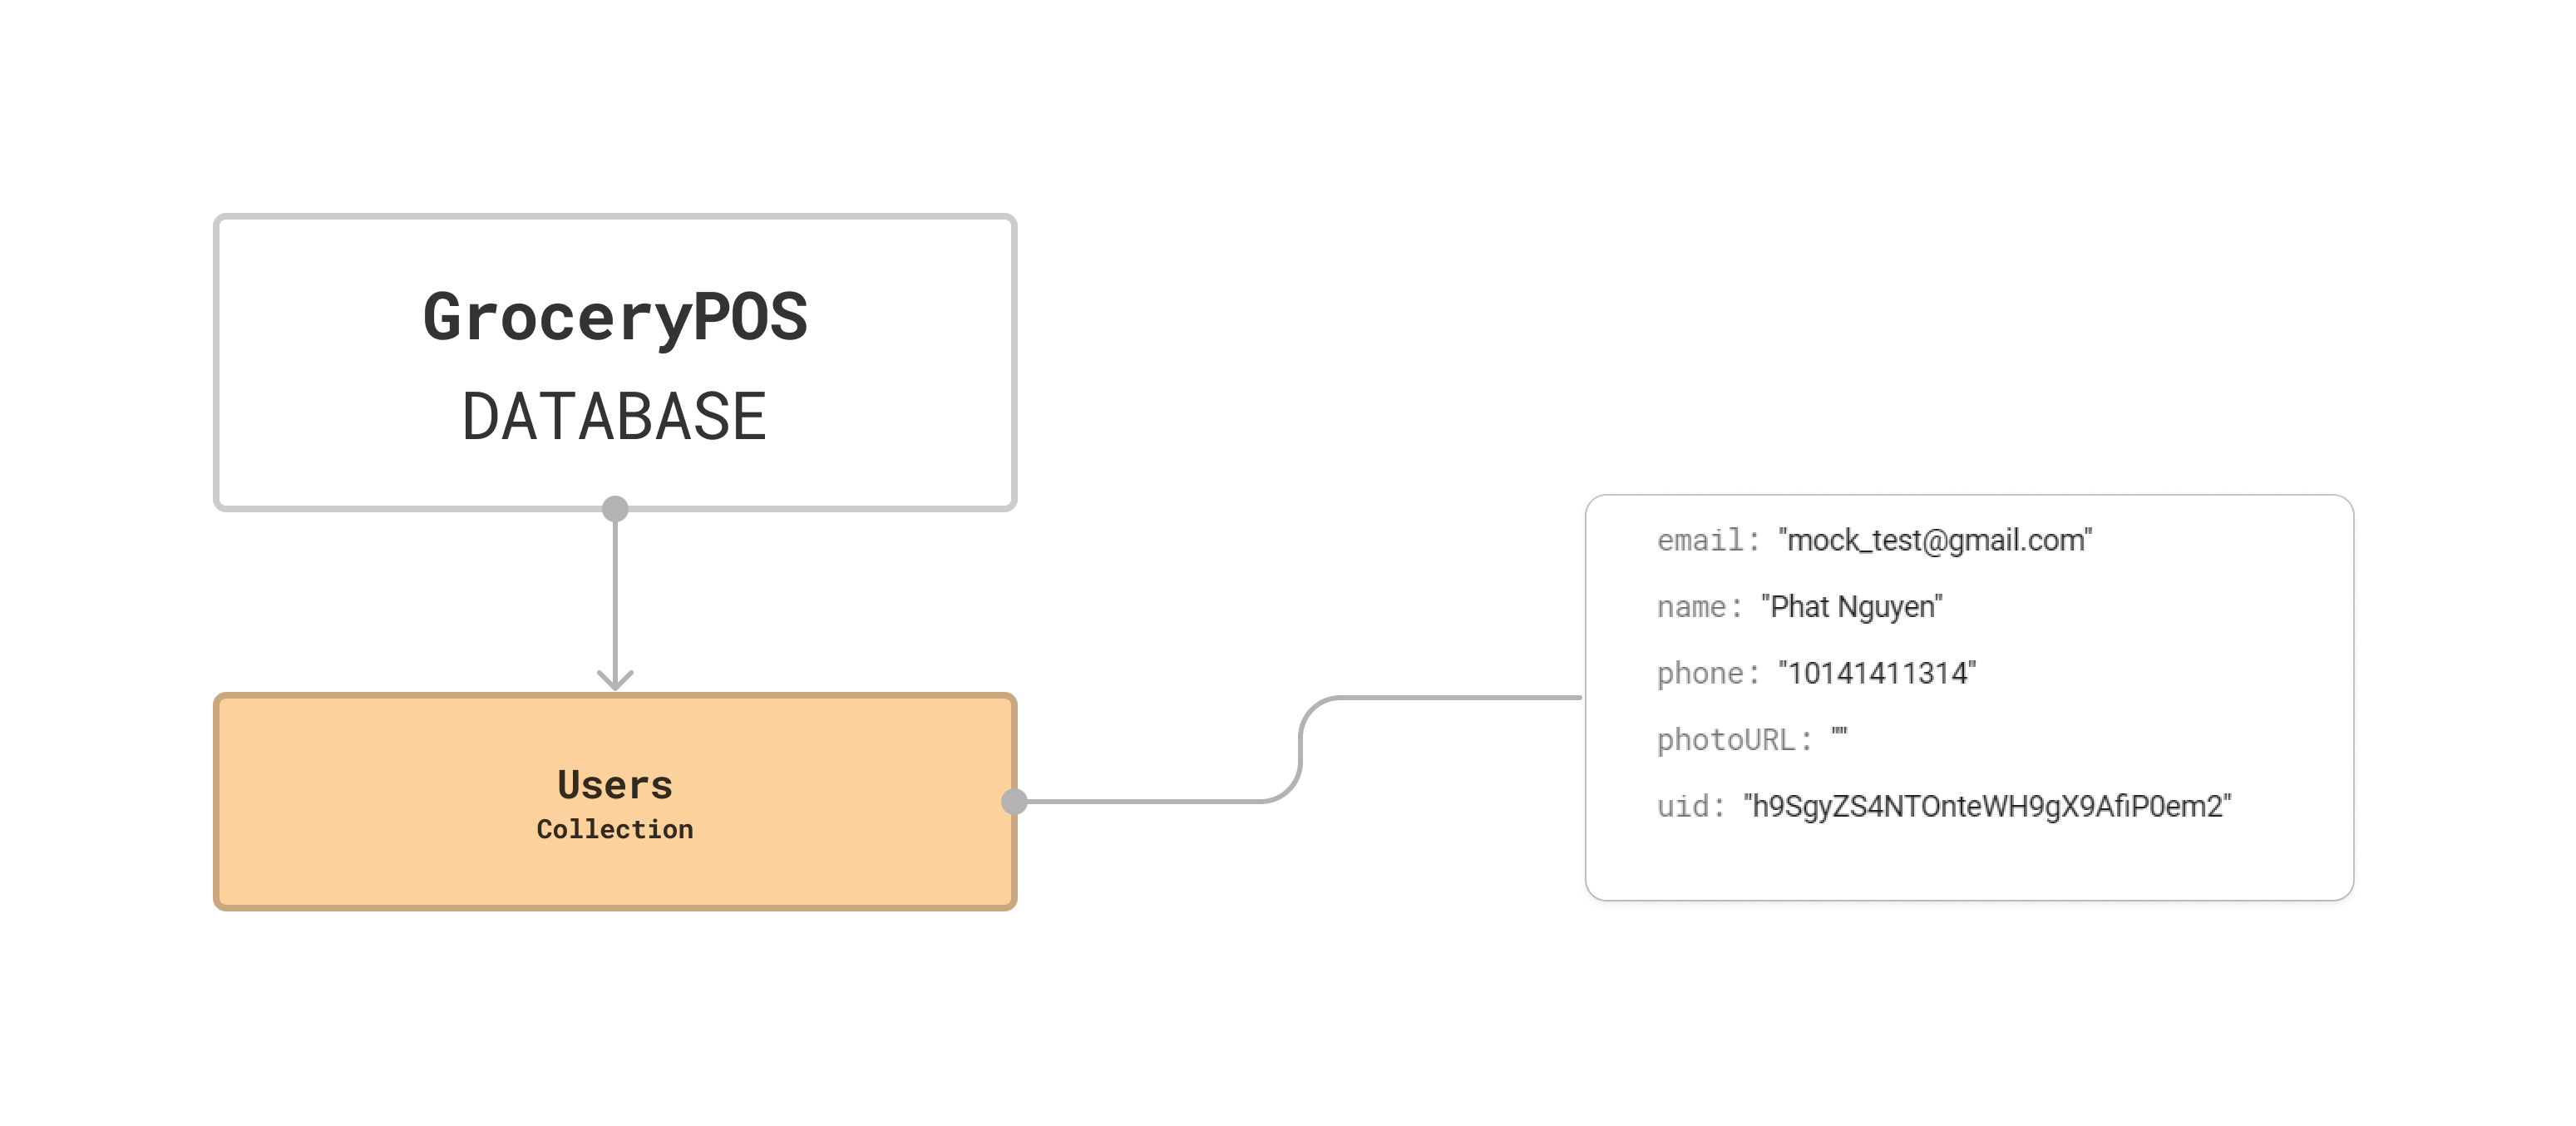
\includegraphics[width=0.9\textwidth]{images/Firestore_UserCollections.png}
    \caption{Firestore: User Collections}
    \label{fig:Firestore_UserCollections}
\end{figure}

\subsubsection*{The Subcollections:}
\begin{figure}[H]
    \centering
    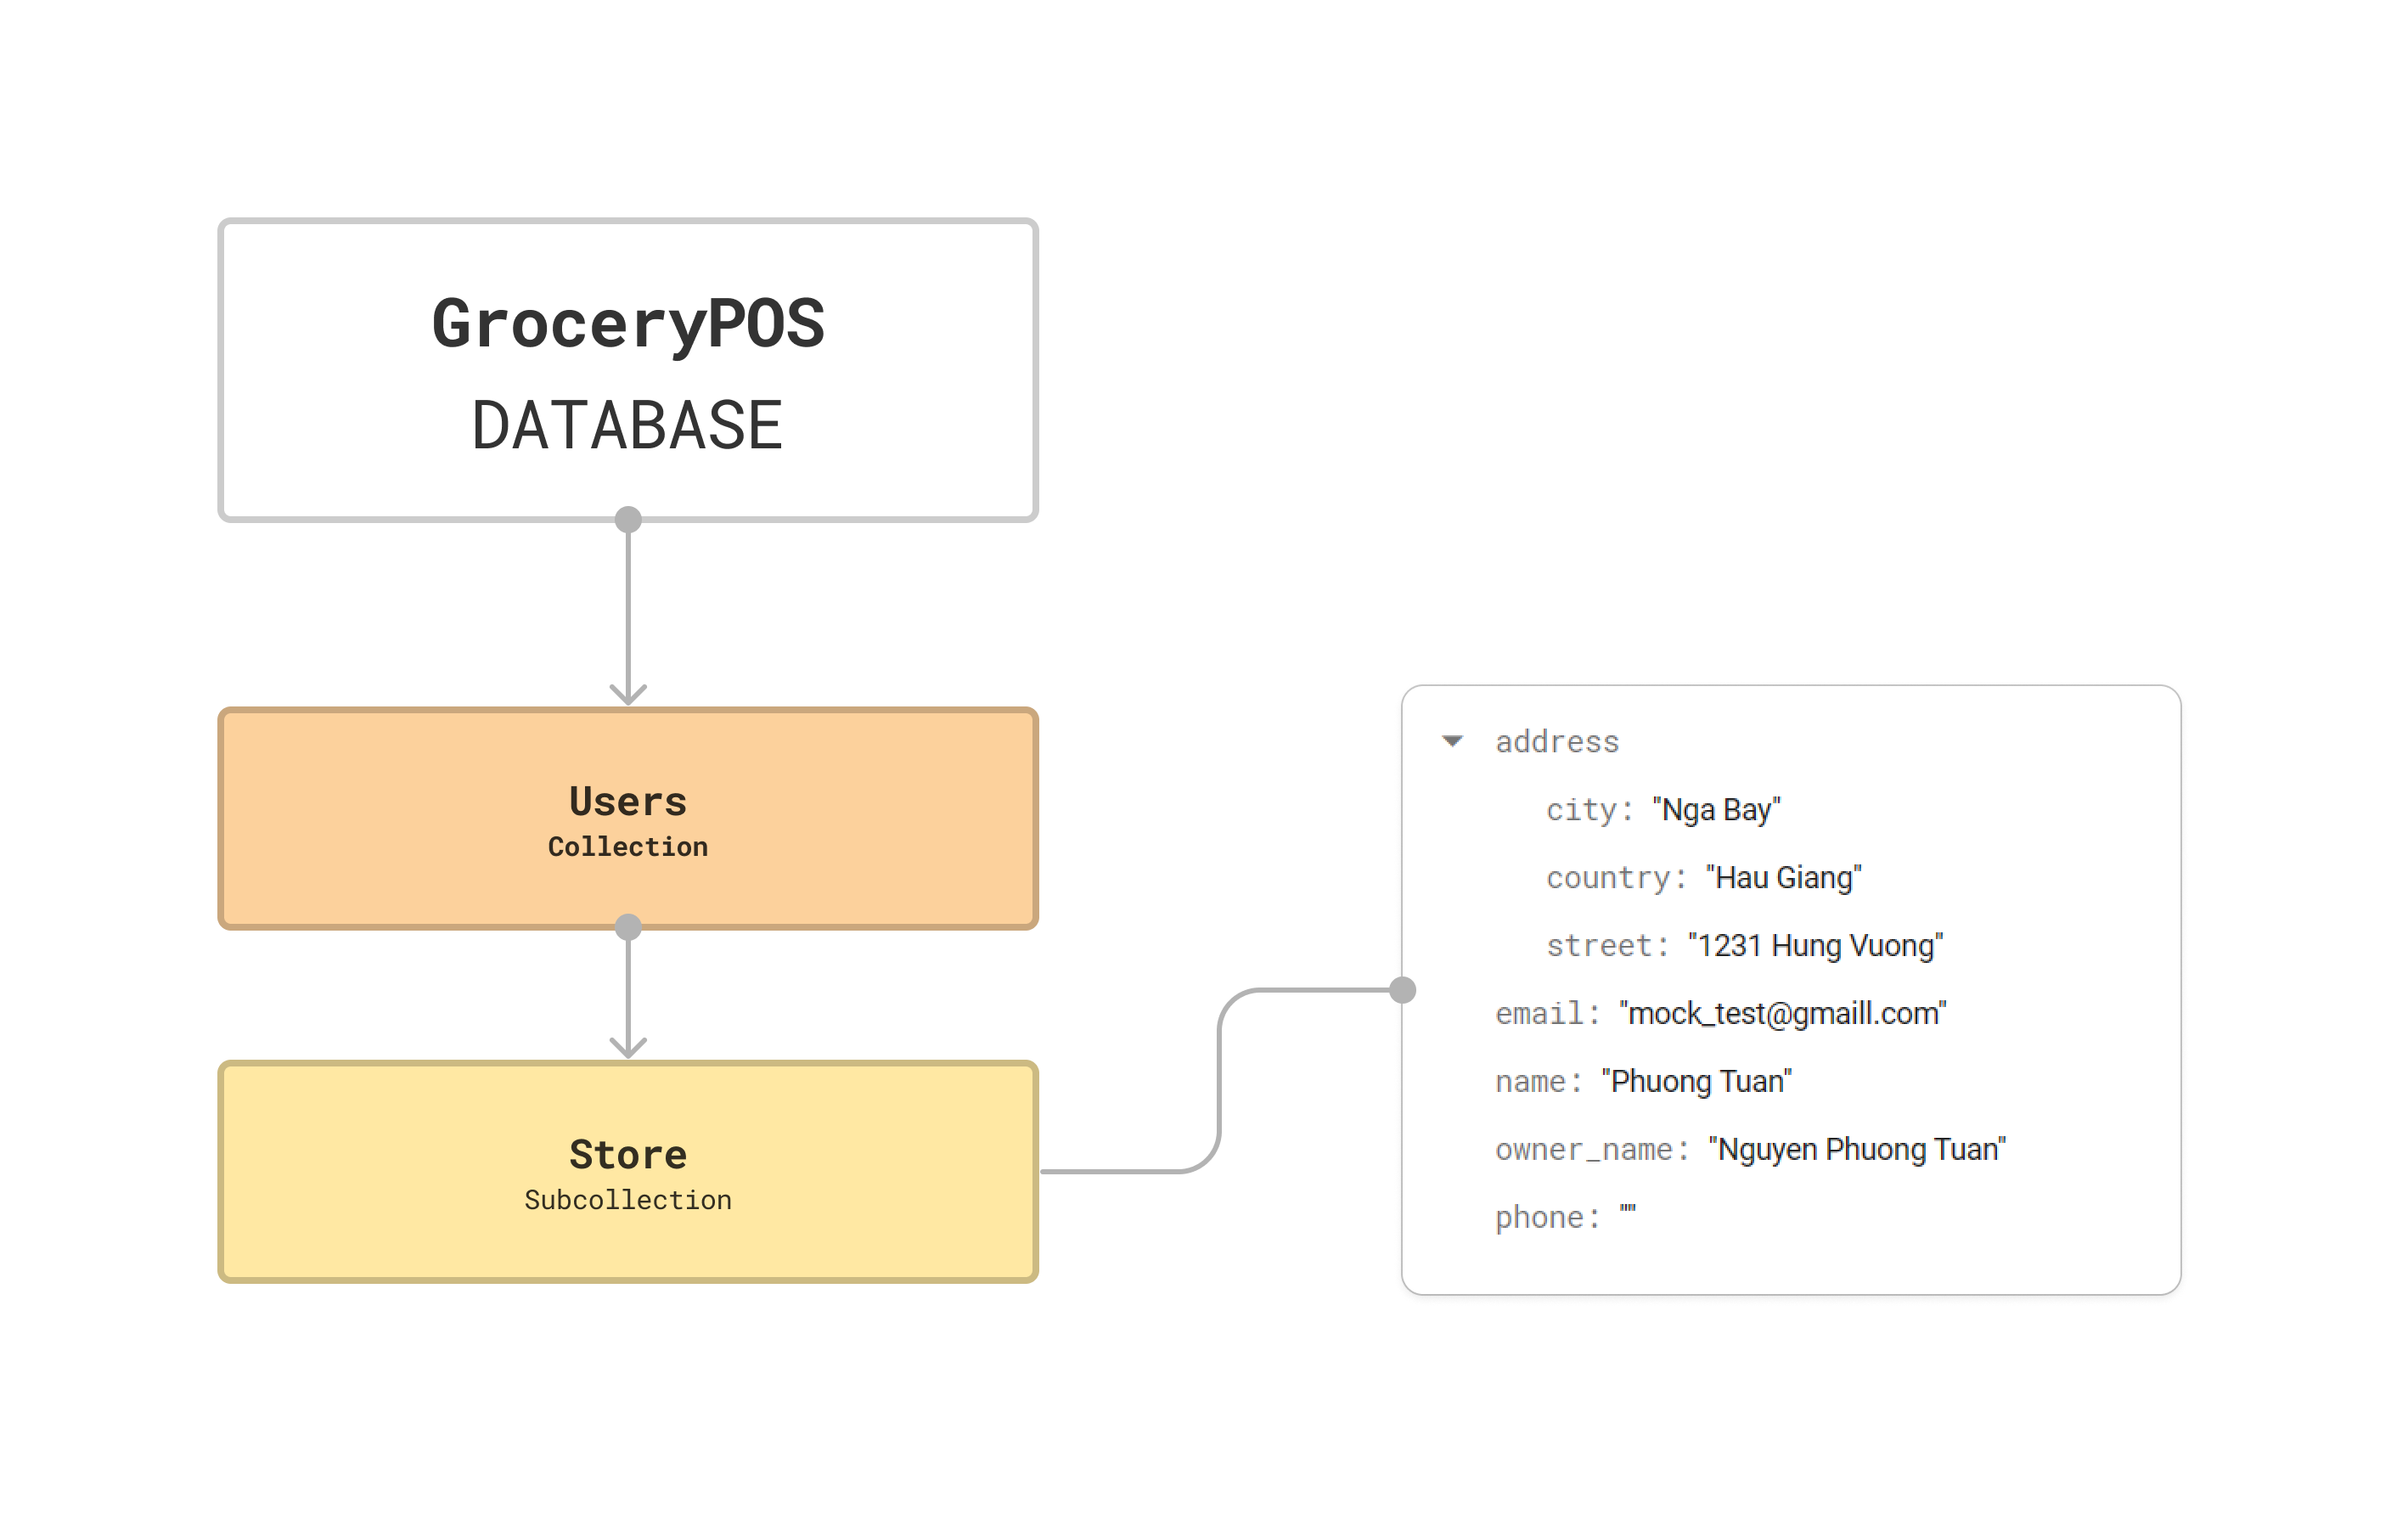
\includegraphics[width=0.9\textwidth]{images/Firestore_StoreCollections.png}
    \caption{Firestore: Store Profile Collections}
    \label{fig:Firestore_StoreCollections}
\end{figure}
\begin{figure}[H]
    \centering
    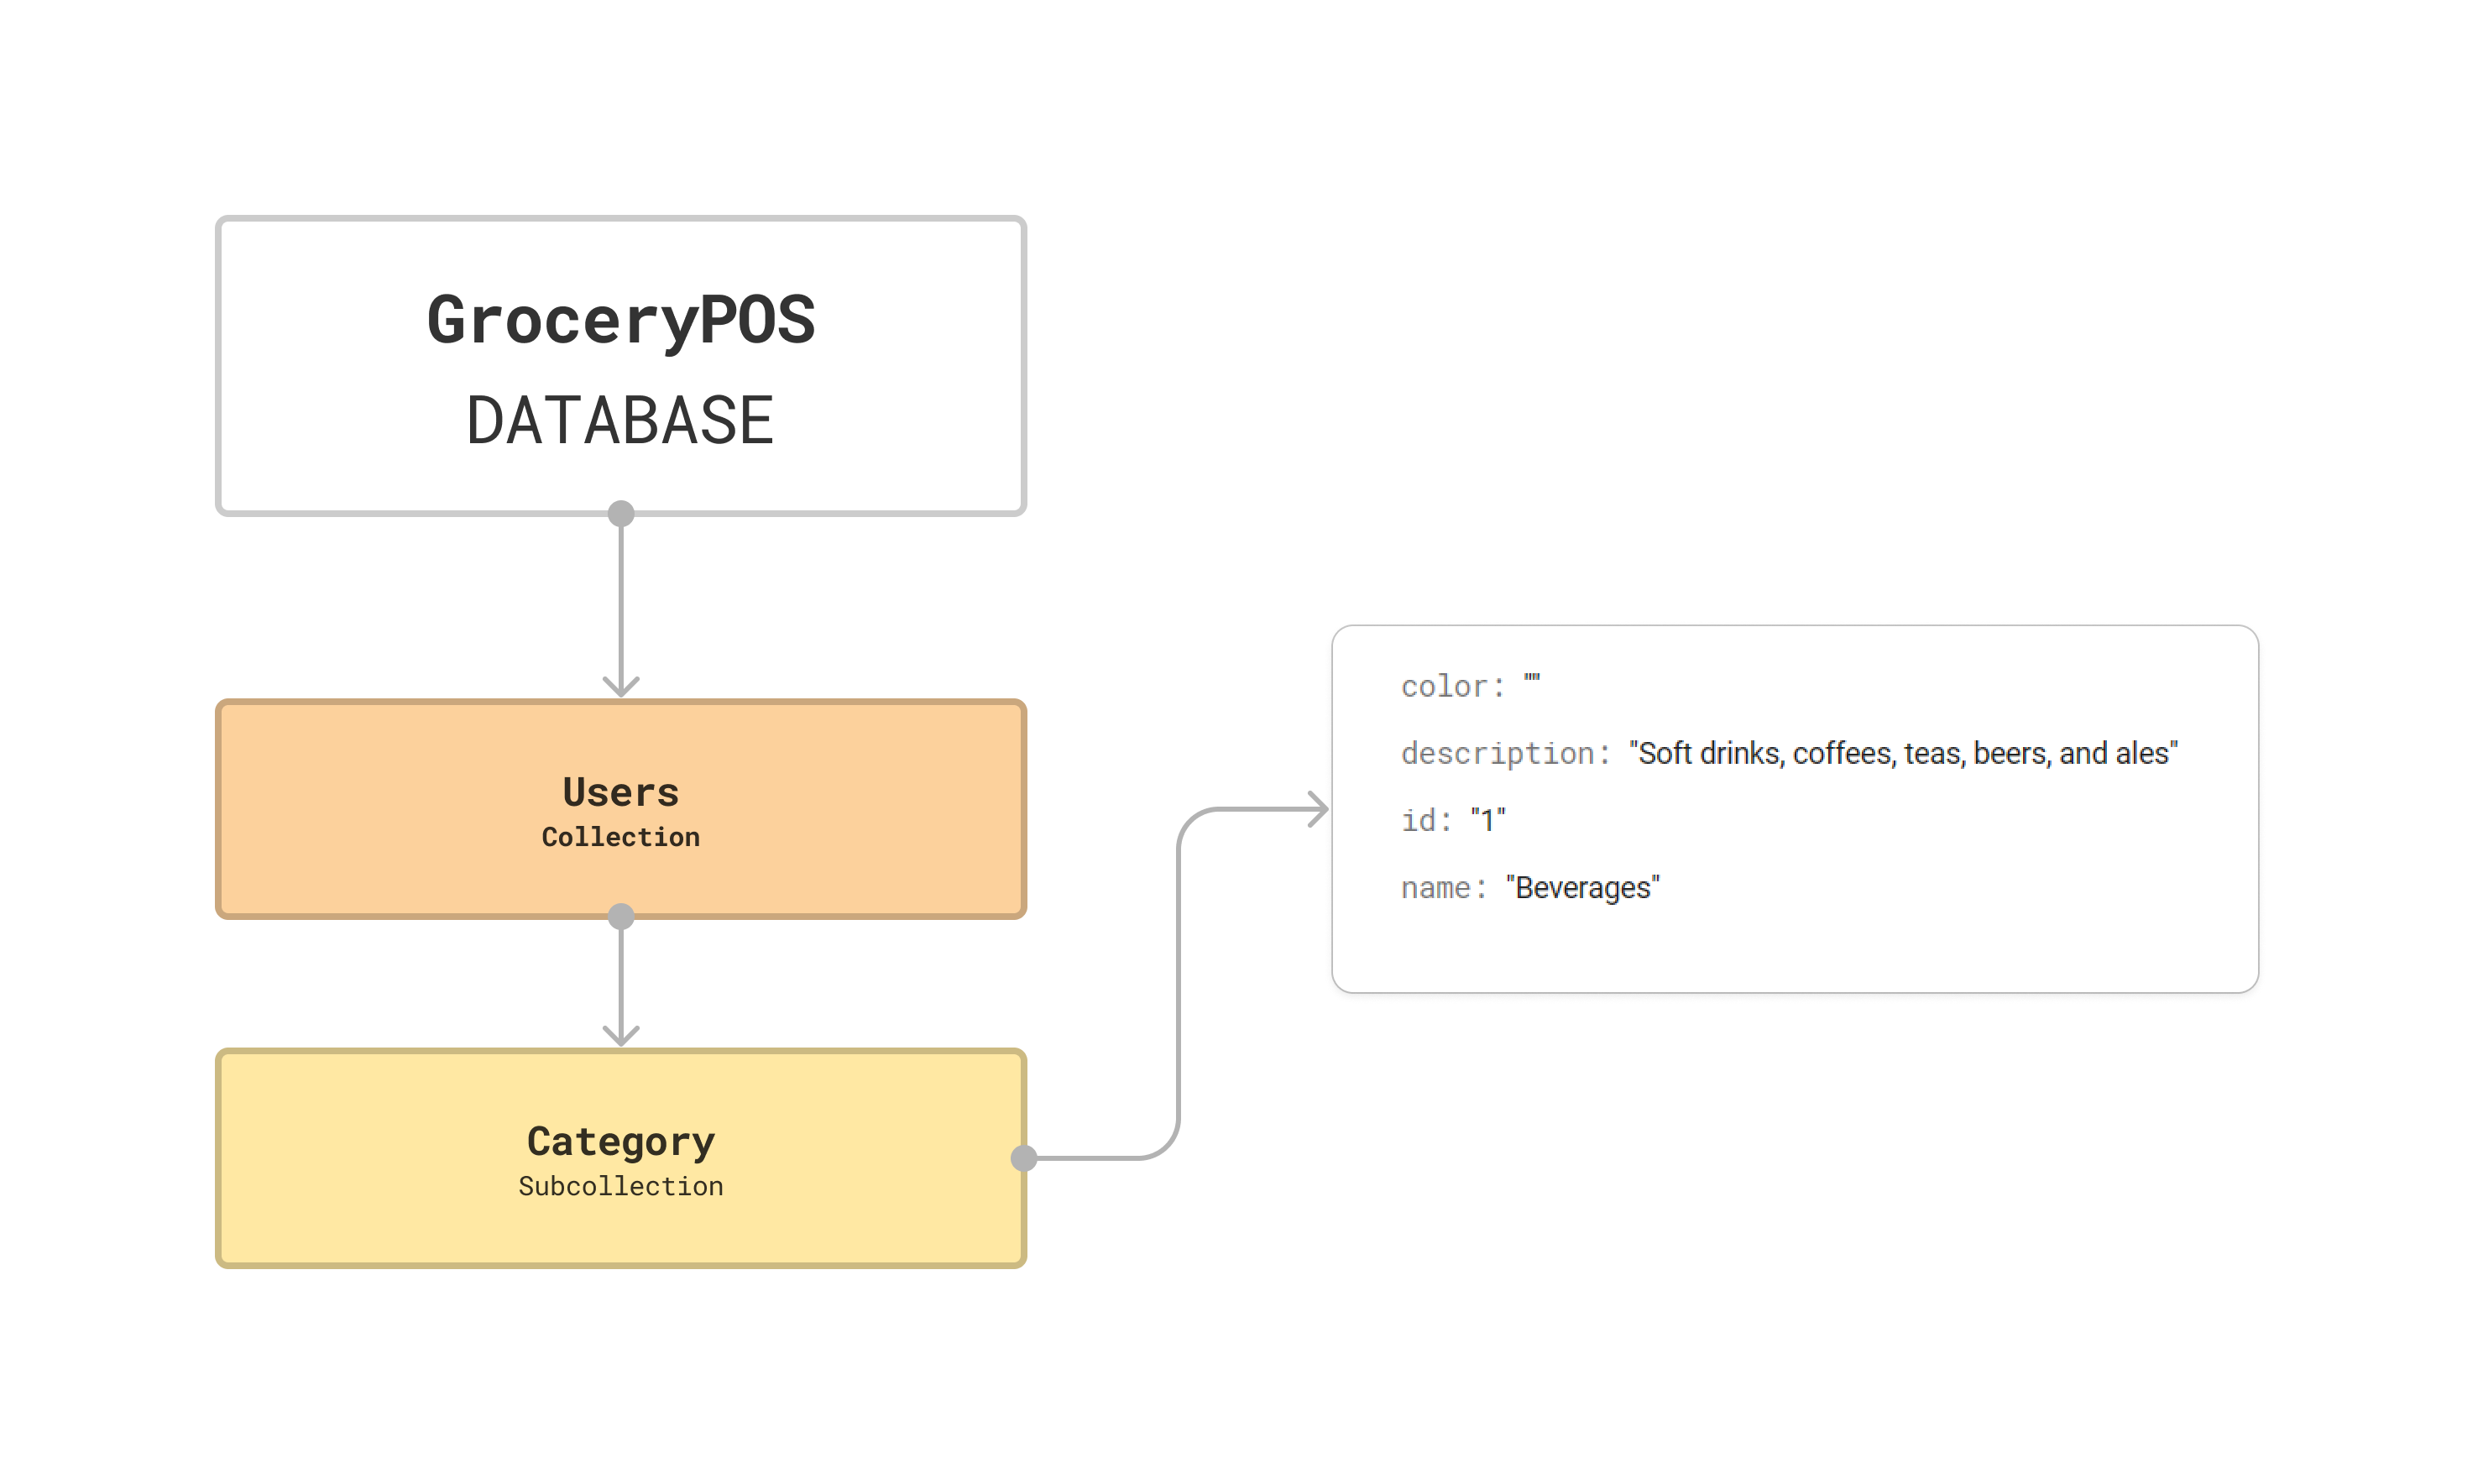
\includegraphics[width=0.9\textwidth]{images/Firestore_CategoryCollections.png}
    \caption{Firestore: Categories Collections}
    \label{fig:Firestore_CategoryCollections}
\end{figure}

\begin{figure}[H]
    \centering
    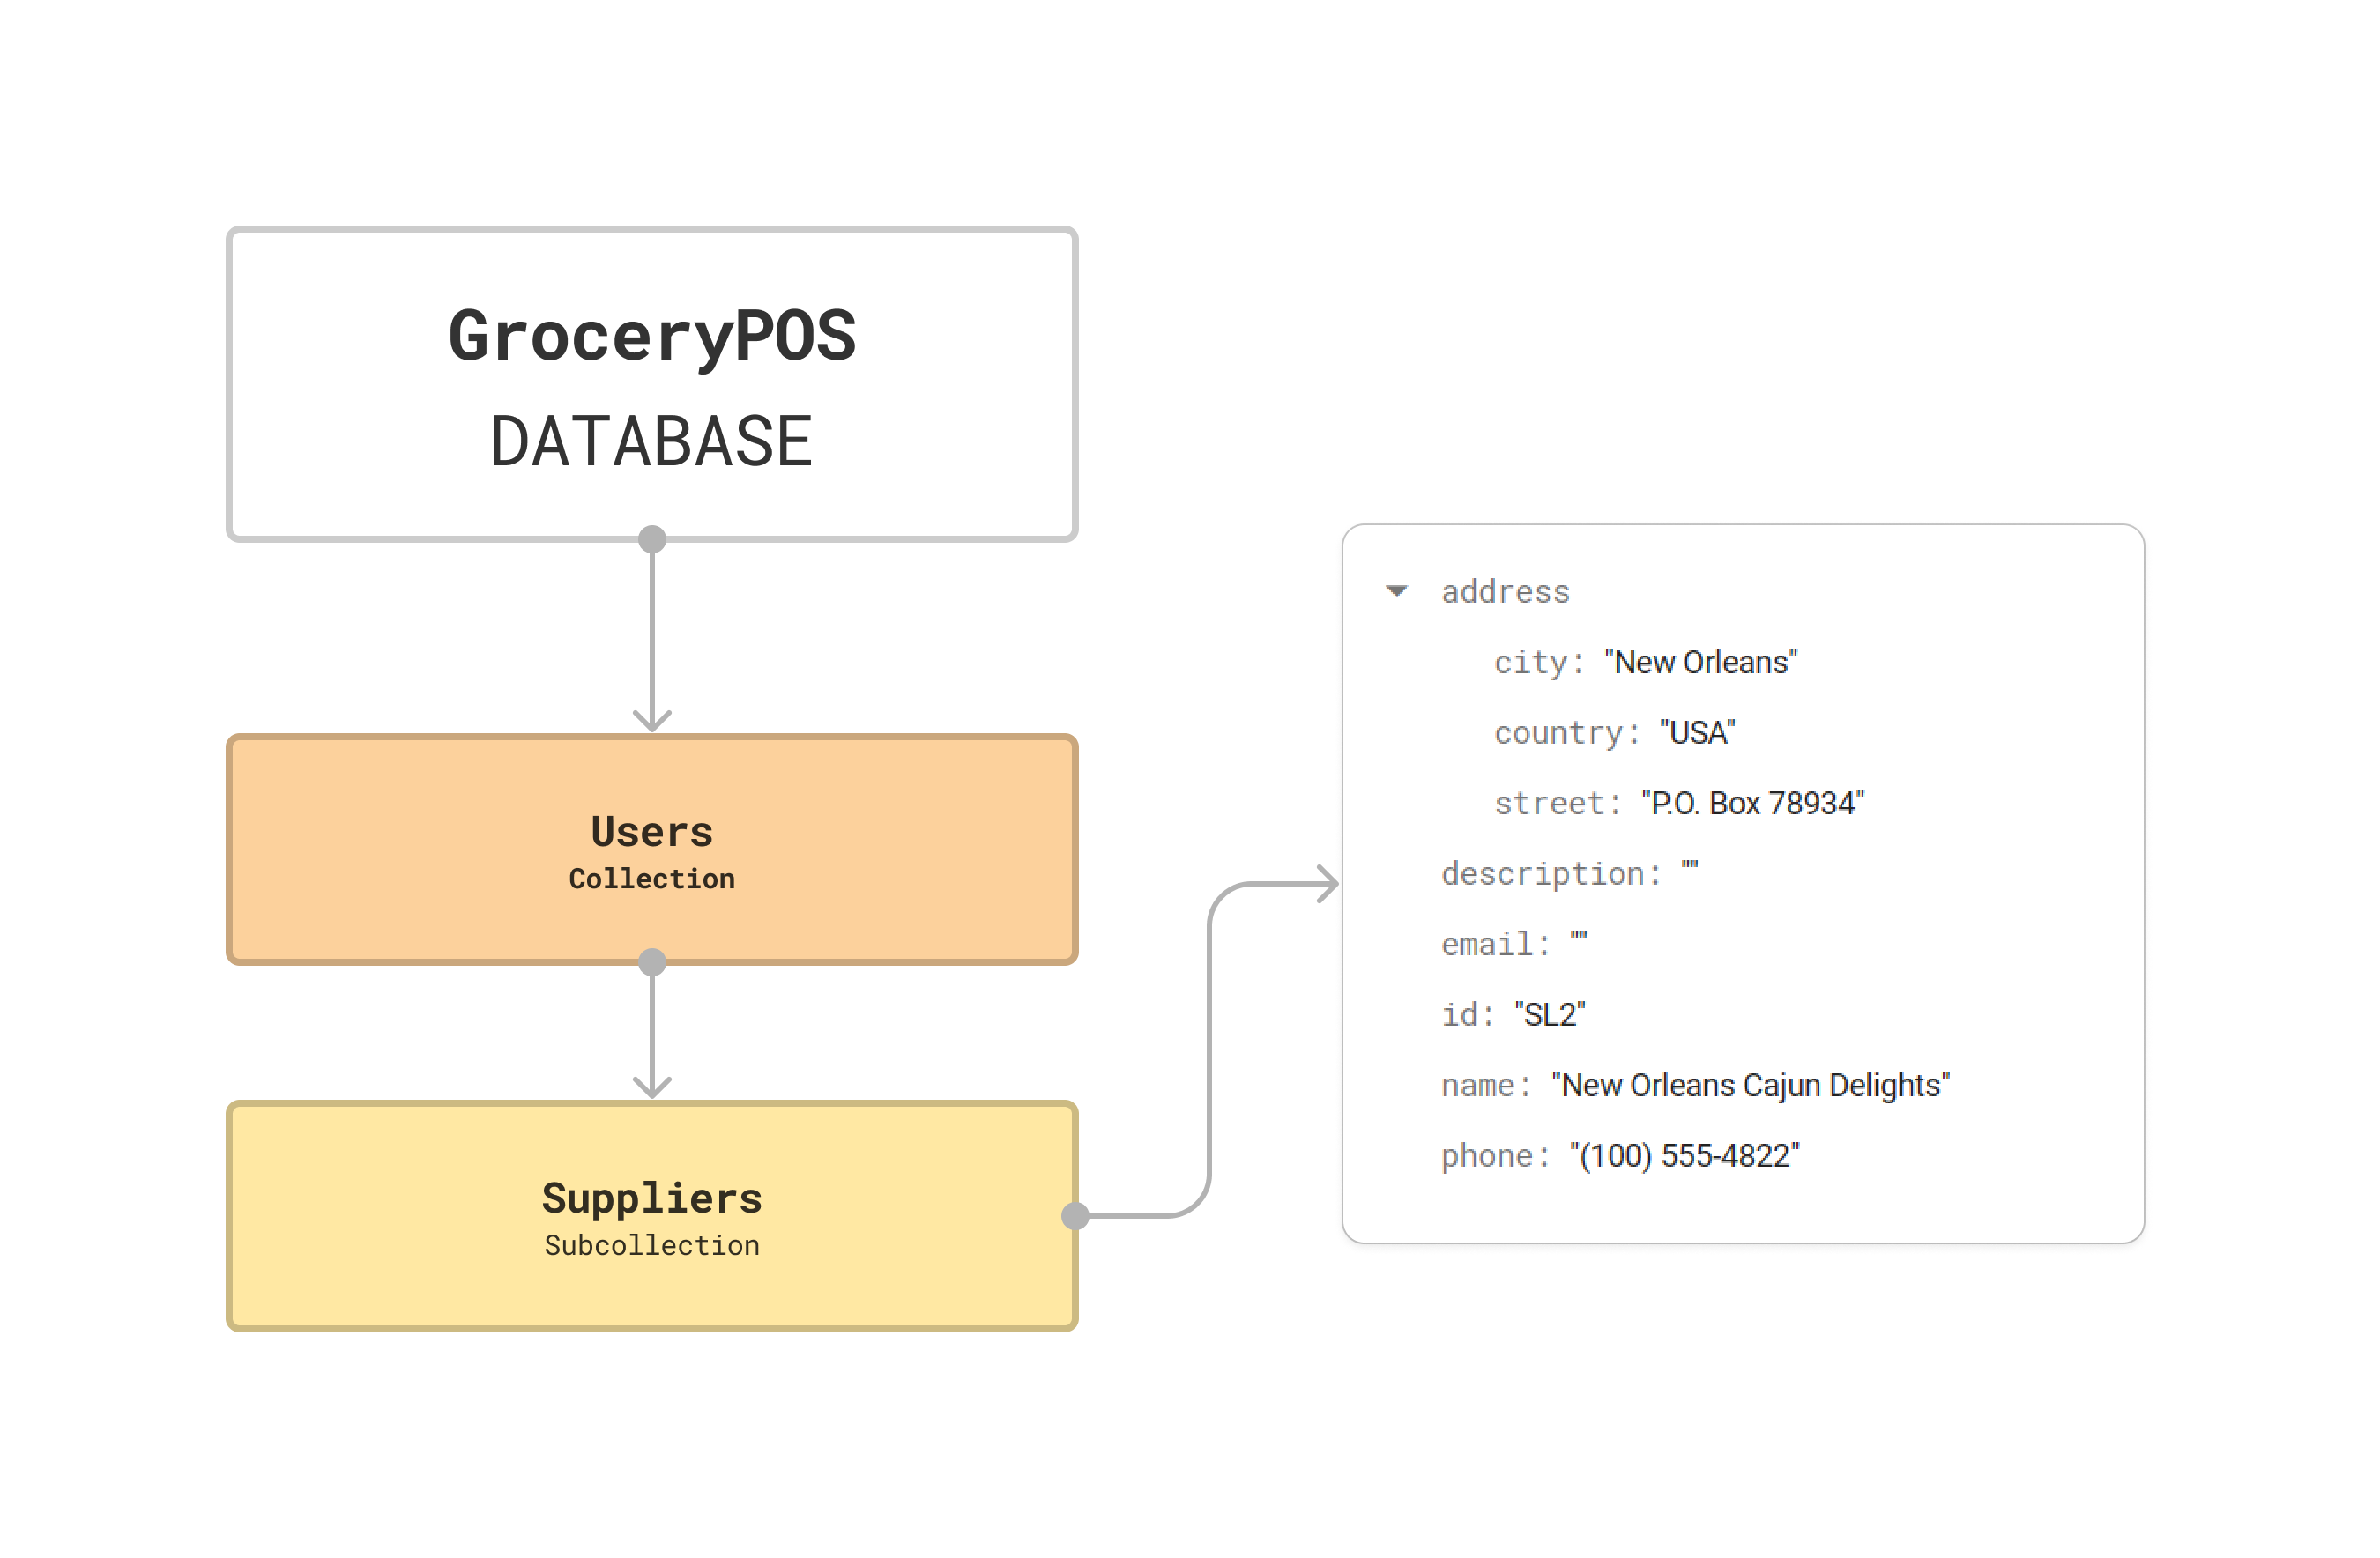
\includegraphics[width=0.9\textwidth]{images/Firestore_SuppliersCollections.png}
    \caption{Firestore: Suppliers Collections}
    \label{fig:Firestore_SuppliersCollections}
\end{figure}

\begin{figure}[H]
    \centering
    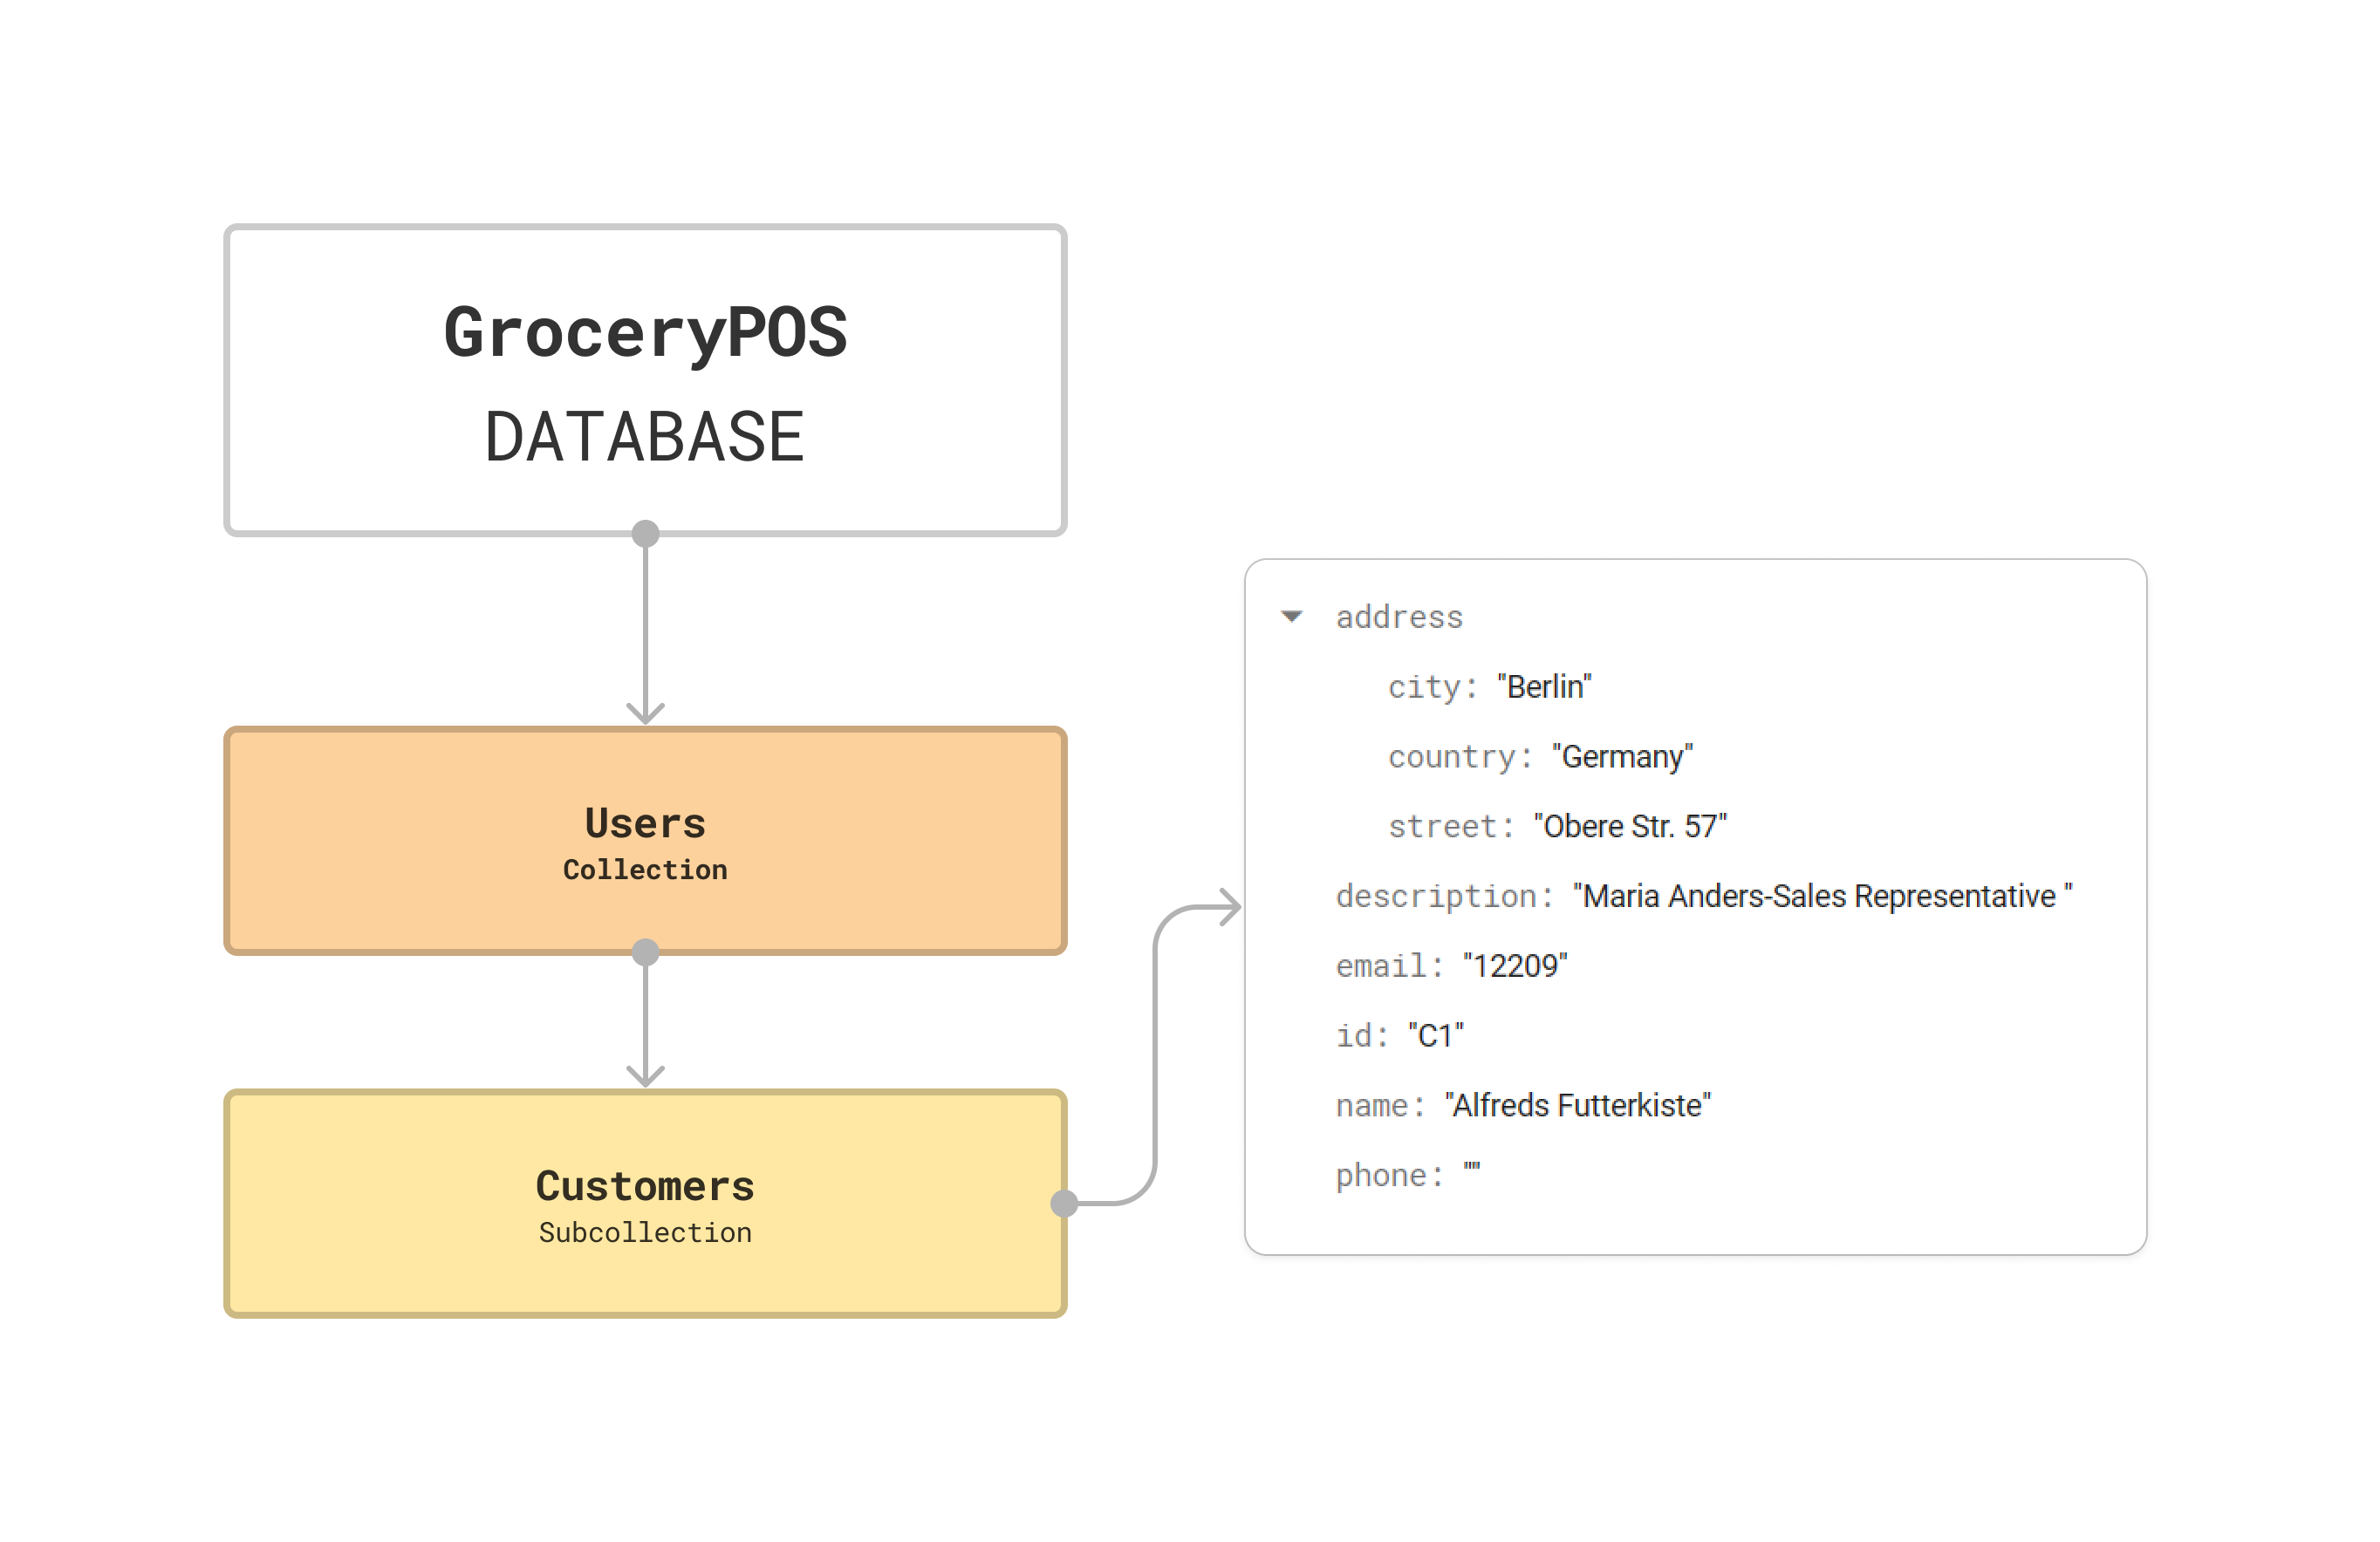
\includegraphics[width=0.85\textwidth]{images/Firestore_CustomersCollections.png}
    \caption{Firestore: Customers Collections}
    \label{fig:Firestore_CustomersCollections}
\end{figure}

\begin{figure}[H]
    \centering
    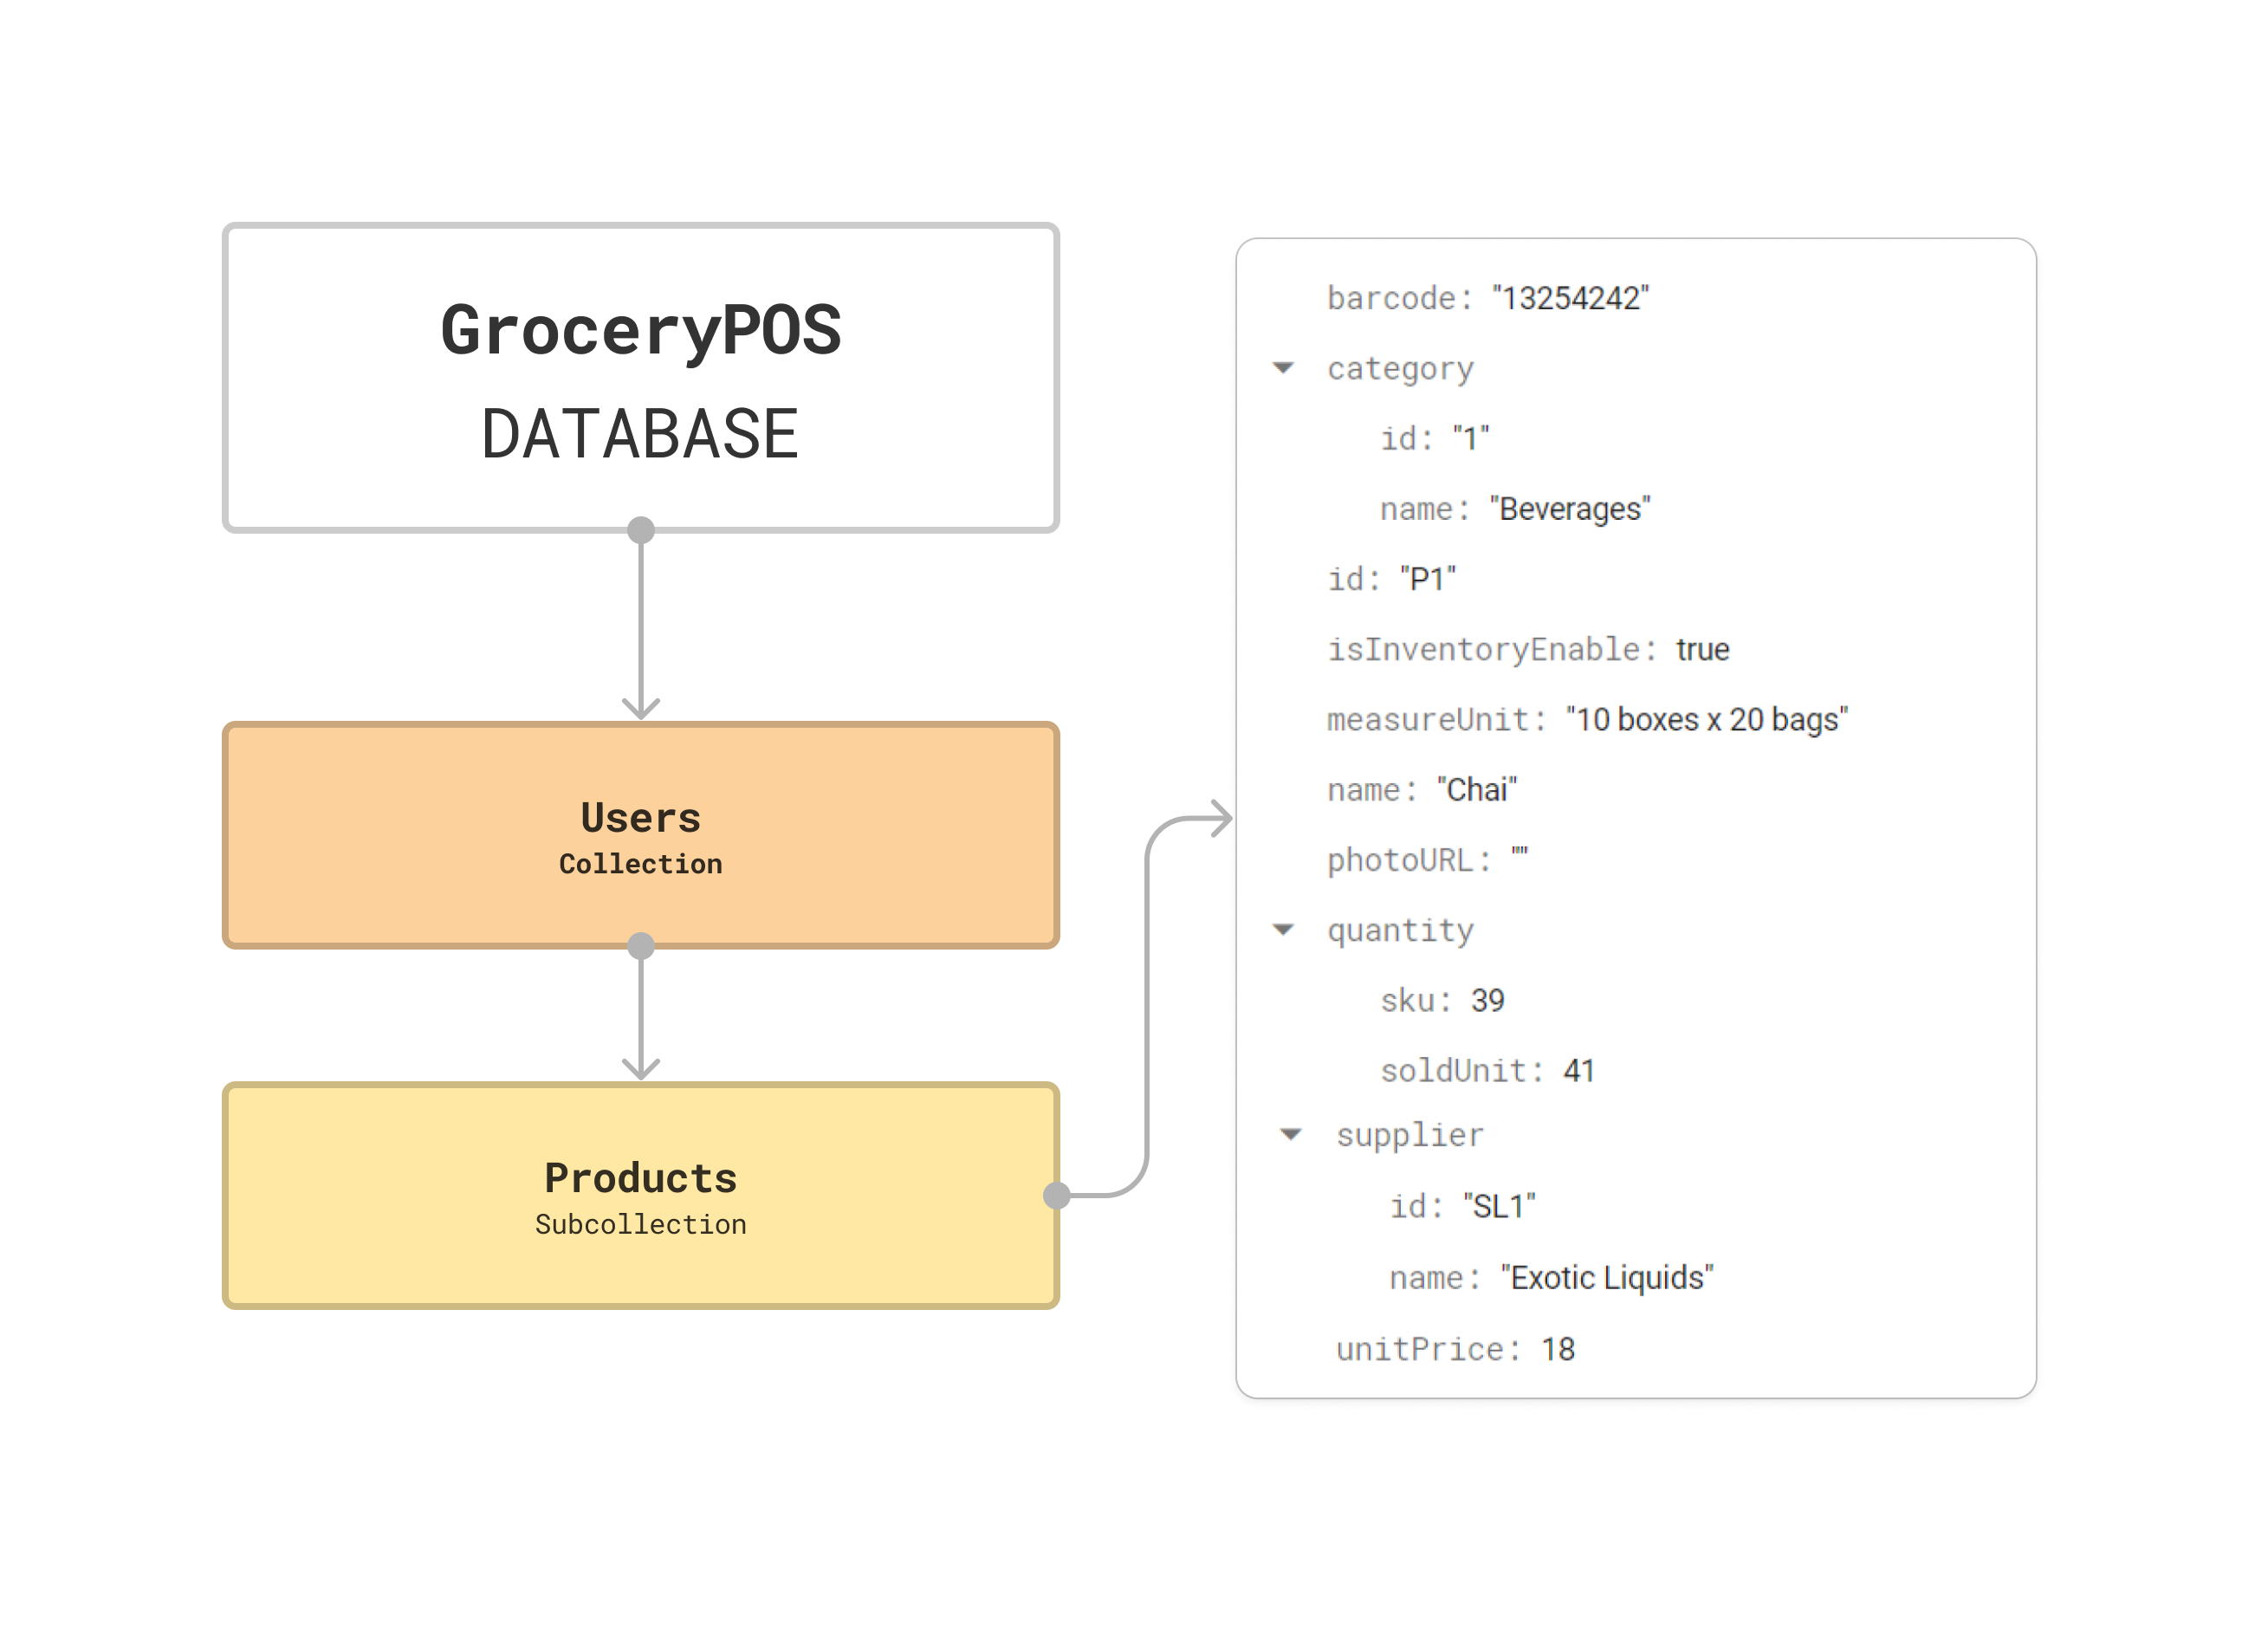
\includegraphics[width=0.85\textwidth]{images/Firestore_ProductsCollections.png}
    \caption{Firestore: Products Collections}
    \label{fig:Firestore_ProductsCollections}
\end{figure}

\begin{figure}[H]
    \centering
    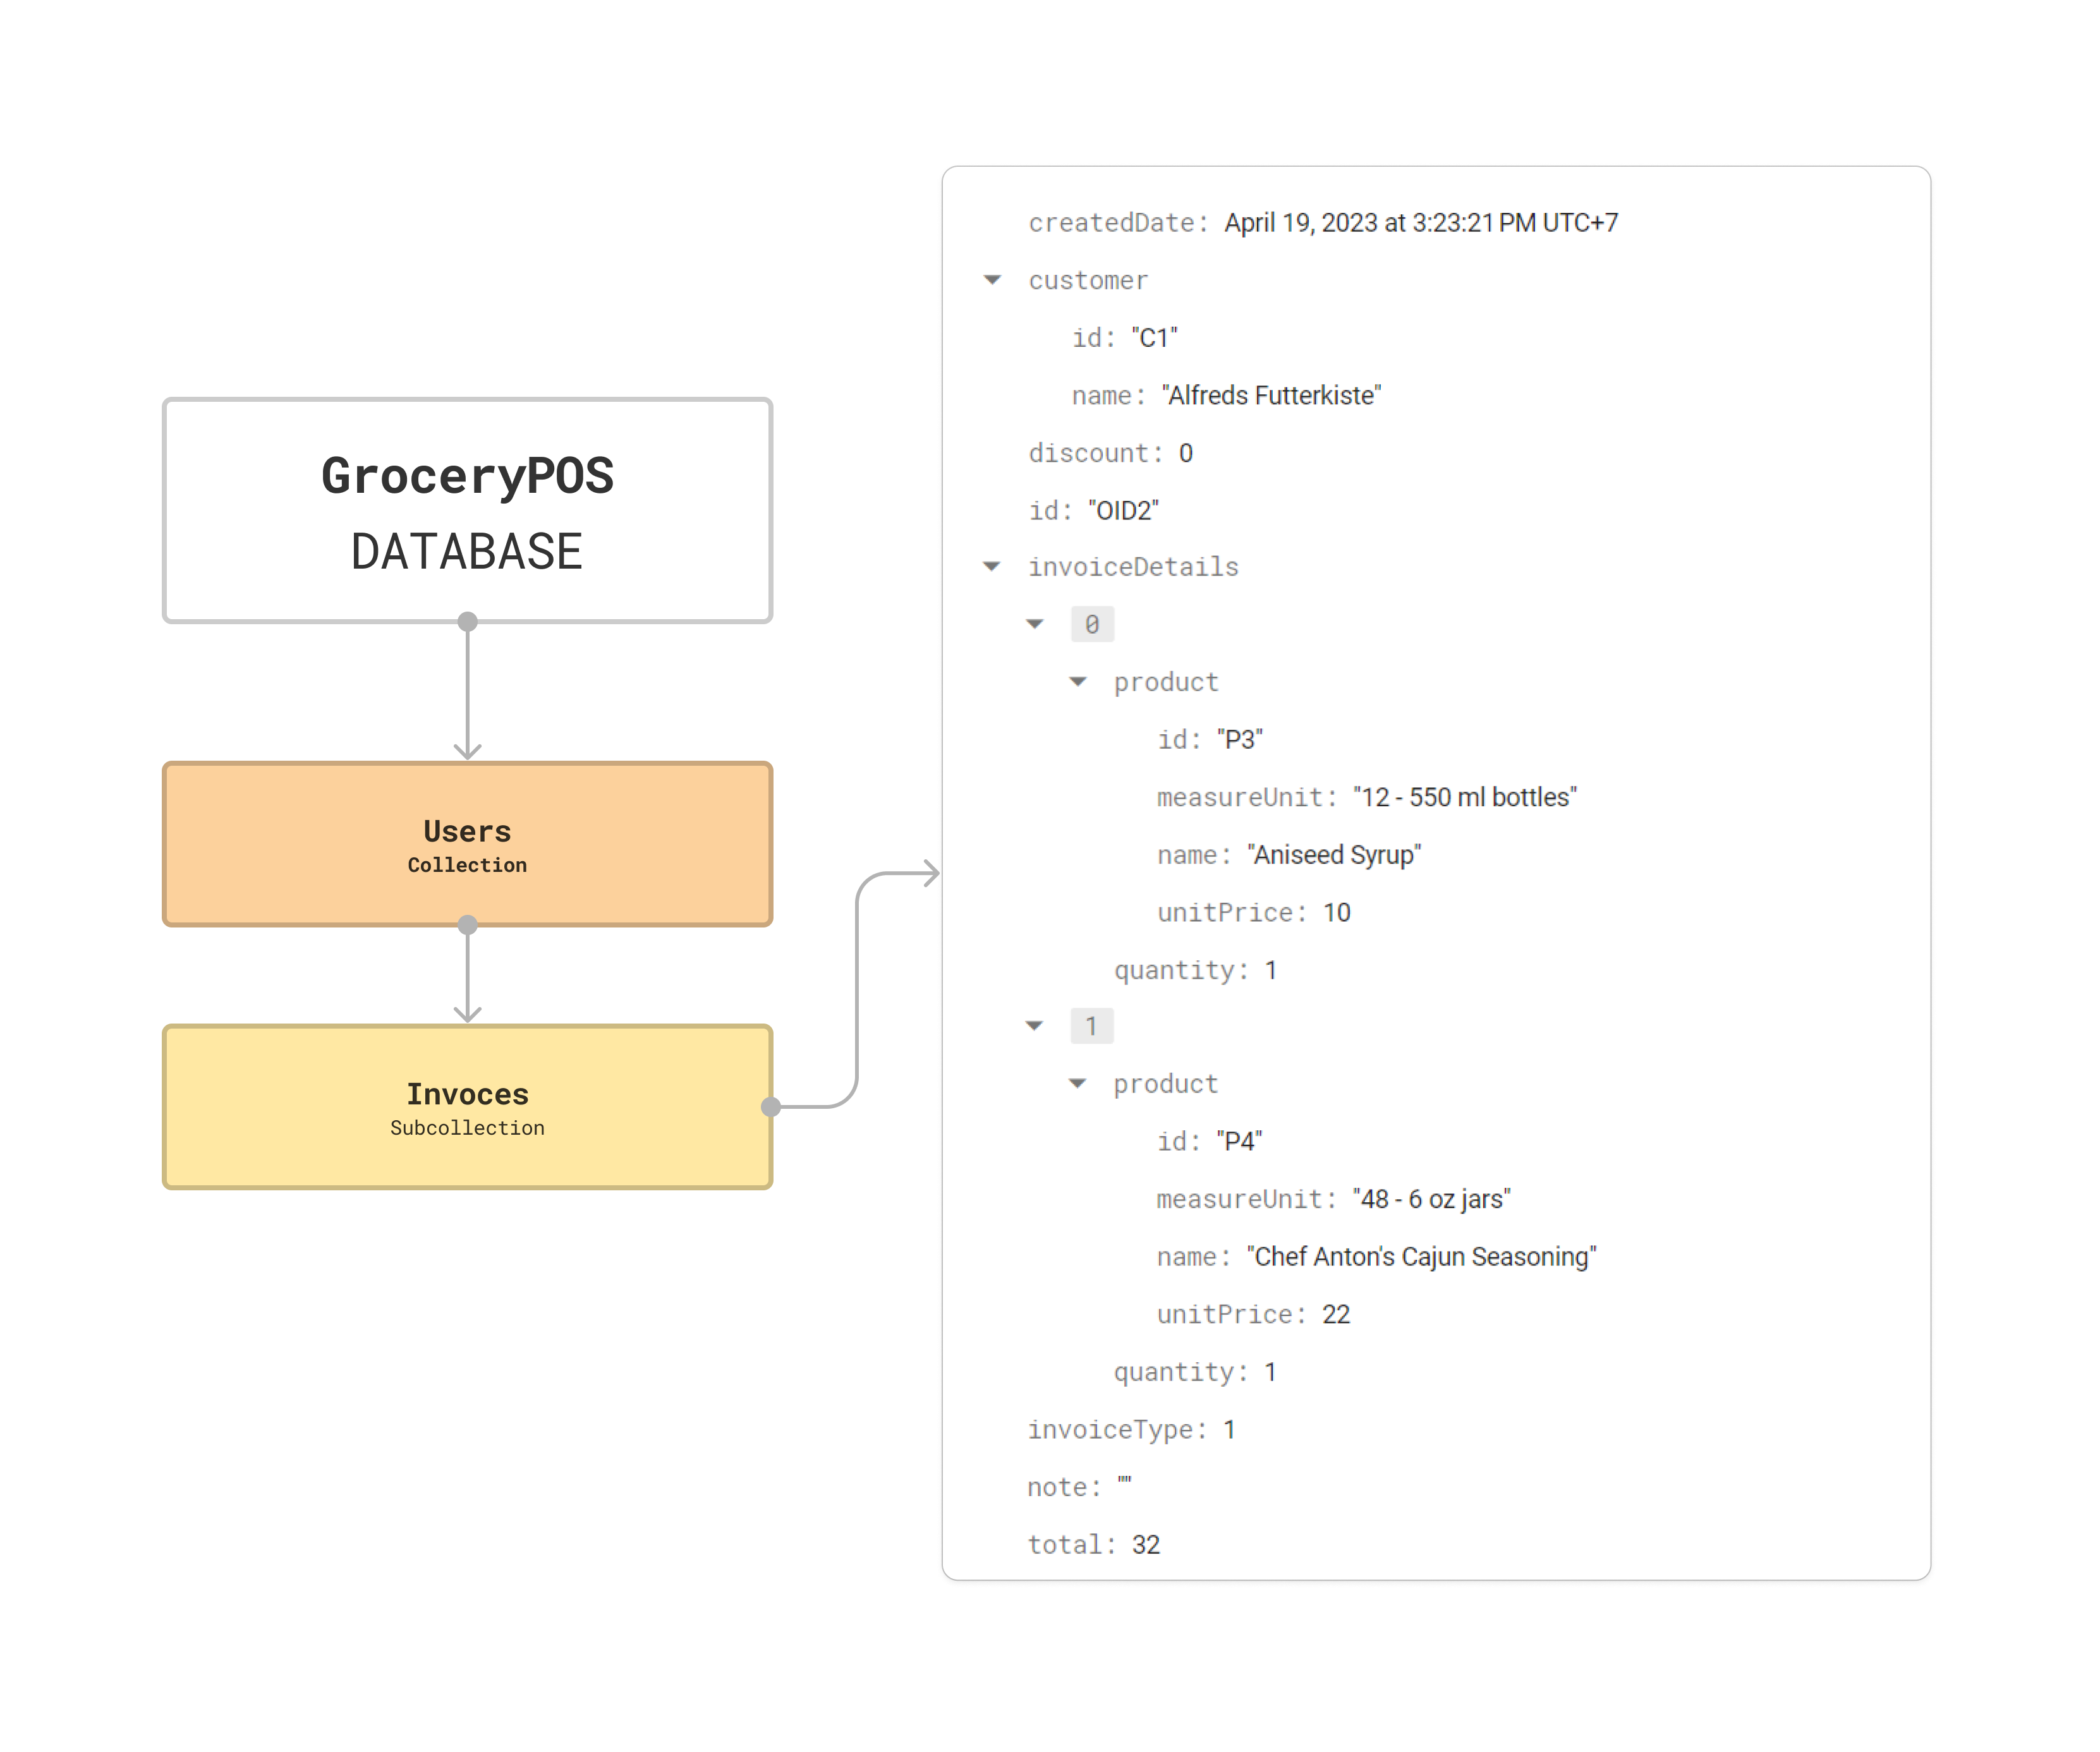
\includegraphics[width=0.8\textwidth]{images/Firestore_InvoicesCollections.png}
    \caption{Firestore: Invoices Collections}
    \label{fig:Firestore_InvoicesCollections}
\end{figure}
\subsection{Data Dictionary}
% \usepackage{graphicx}



\begin{center}
    \begin{table}[H]

        \resizebox{\textwidth}{!}{%
            \normalsize
            \begin{tabular}{|l|l|l|} \hline
                \textbf{Data} & \textbf{Type} & \textbf{Description}             \\ \hline
                user\_uid     & String~       & The user authentication
                auto-generated ID by Firebase Authentication                     \\ \hline
                name          & String~       & The fullname of the user in
                profile.                                                         \\ \hline
                email         & String~       & The email which provided for the
                User Authentication                                              \\ \hline
                phone         & String~       & The phone for OTP athuentication
                in register.                                                     \\ \hline
                photoURL      & String~       & The reference to the user
                profile's in Google Cloud                                        \\ \hline
            \end{tabular}%

        }
        \caption{Data Description: User}
        \label{tab:table-data-description-user}


    \end{table}
\end{center}

\begin{center}
    \begin{table}[H]

        \resizebox{\textwidth}{!}{%
            \normalsize
            \begin{tabular}{|l|l|l|} \hline
                \textbf{Data}          & \textbf{Type} & \textbf{Description}             \\ \hline
                category\_id           & String        & The unique ID to identify the
                category                                                                  \\ \hline
                category\_name         & String        & The name of category.            \\ \hline
                category\_description~ & String        & The detail information about
                category.                                                                 \\ \hline
                category\_color~       & String        & The hex code of color to display
                the category.                                                             \\ \hline
            \end{tabular}%

        }
        \caption{Data Description: Category}
        \label{tab:table-data-description-category}


    \end{table}
\end{center}

\begin{center}
    \begin{table}[H]

        \resizebox{\textwidth}{!}{%
            \normalsize
            \begin{tabular}{|l|l|l|} \hline
                \textbf{Data}         & \textbf{Type} & \textbf{Description}             \\ \hline
                supplier\_id          & String        & The unique ID to identify the
                suppier.                                                                 \\ \hline
                supplier\_name        & String        & The name of suppliers.           \\ \hline
                supplier\_email       & String        & The email to contact suppliers.  \\ \hline
                supplier\_phone       & String        & The number to contact suppliers. \\ \hline
                supplier\_description & String        & The detail information about
                supplier.                                                                \\ \hline
                supplier\_address     & Map           & The address to retrivie directed
                contact suppliers                                                        \\ \hline
                supplier\_street      & String        & The detail of address.           \\ \hline
                supplier\_city        & String        & The detail of address.           \\ \hline
                supplier\_country     & String        & The detail of address.           \\ \hline
            \end{tabular}%

        }
        \caption{Data Description: Suppliers}
        \label{tab:table-data-descriptionr-suppliers}


    \end{table}
\end{center}

\begin{center}
    \begin{table}[H]

        \resizebox{\textwidth}{!}{%
            \normalsize
            \begin{tabular}{|l|l|l|} \hline
                \textbf{Data}         & \textbf{Type} & \textbf{Description}             \\ \hline
                customer\_id          & String        & The unique ID to identify the
                customer.                                                                \\ \hline
                customer\_name        & String        & The name of customers.           \\ \hline
                customer\_email       & String        & The email to contact customers.  \\ \hline
                customer\_phone       & String        & The number to contact customers. \\ \hline
                customer\_description & String        & The detail information about
                customer.                                                                \\ \hline
                customer\_address     & Map           & The address to retrivie directed
                contact customers                                                        \\ \hline
                customer\_street      & String        & The detail of address.           \\ \hline
                customer\_city        & String        & The detail of address.           \\ \hline
                customer\_country     & String        & The detail of address.           \\ \hline
            \end{tabular}%

        }
        \caption{Data Description: Category}
        \label{tab:table-data-description-customers}


    \end{table}
\end{center}


\begin{center}
    \begin{table}[H]

        \resizebox{\textwidth}{!}{%
            \normalsize
            \begin{tabular}{|l|l|l|} \hline
                \textbf{Data}           & \textbf{Type} & \textbf{Description}             \\ \hline
                product\_id             & String        & The unique ID to identify the
                invoices.                                                                  \\ \hline
                product\_barcode        & String        & The barcode of product.          \\ \hline
                product\_name           & String        & The name of product.             \\ \hline
                product\_measureUnit    & String        & The means of measurement of
                product.                                                                   \\ \hline
                product\_unitPrice      & Number        & The price of product per measure
                unit.                                                                      \\ \hline
                product\_photoURL       & String        & The reference to Google Cloud to
                retrive photo.                                                             \\ \hline
                product\_quanity        & map           & The inventory quantity of the
                product.                                                                   \\ \hline
                product\_sku            & Number        & The number of stock on unit of
                product                                                                    \\ \hline
                product\_soldUnit       & Number        & The number of sold unit of
                product                                                                    \\ \hline
                product\_supplier       & map           & The map to use reference
                Supplier Collections                                                       \\ \hline
                product\_supplier\_id   & String        & The id of Supplier.              \\ \hline
                product\_supplier\_name & String        & The name of Supplier.            \\ \hline
                product\_category       & map           & The map to use reference
                Category Collections                                                       \\ \hline
                product\_category\_id   & String        & The id of Category.              \\ \hline
                product\_category\_name & String        & The name of Category.            \\ \hline
            \end{tabular}%

        }
        \caption{Data Description: Product}
        \label{tab:table-data-description-product}


    \end{table}
\end{center}


\begin{center}
    \begin{table}[H]

        \resizebox{\textwidth}{!}{%
            \normalsize
            \begin{tabular}{|l|l|l|} \hline
                \textbf{Data}             & \textbf{Type} & \textbf{Description}            \\ \hline
                invoice\_id               & String        & The unique ID to identify the
                invoices.                                                                   \\ \hline
                invoice\_createdDate      & Timestamp     & The timestamp when the invoice
                created                                                                     \\ \hline
                invoice\_discount         & Number        & The discount of invoice.        \\ \hline
                invoice\_note             & String        & The note of invoice.            \\ \hline
                invoice\_total            &               & The total cost of invoice.      \\ \hline
                invoice\_invoice\_details & Array         & The list of invoice details of
                invoice.                                                                    \\ \hline
                invoice\_invoiceType      & Number        & The number to identify the type
                of invoice: 0: Retail Invoices, 1: Customer Invoices                        \\ \hline
                invoice\_customer         & Map           & The map to reference
                Customer~ Collections                                                       \\ \hline
                invoice\_customer\_id     & String        & The unique ID to identify the
                customer.                                                                   \\ \hline
                invoice\_customer\_name   & String        & The name of customers.          \\ \hline
            \end{tabular}%

        }
        \caption{Data Description: Invoices}
        \label{tab:table-data-description-inoice}


    \end{table}
\end{center}


\begin{center}
    \begin{table}[H]

        \resizebox{\textwidth}{!}{%
            \normalsize
            \begin{tabular}{|l|l|l|} \hline
                \textbf{Data}        & \textbf{Type} & \textbf{Description}                                 \\ \hline
                product              & map           & The map object to store a copy
                  of Product details  \\ \hline
                product\_id          &               & The map to use reference Product
                  Collections       \\ \hline
                product\_barcode     & String        & The barcode of product.                              \\ \hline
                product\_name        & String        & The name of product.                                 \\ \hline
                product\_measureUnit & String        & The means of measurement of
                  product.               \\ \hline
                proudct\_unitPrice   & Number        & The price of product per measure
                  unit.             \\ \hline
                quantity             & Number        & The quantity of product in that invoice             \\ \hline
            \end{tabular}%

        }
        \caption{Data Description: invoices}
        \label{tab:table-data-description-inoice-detail}


    \end{table}
\end{center}
\section{Detailed Design}
\subsection{User Authentication}
\subsubsection{Login View}

\begin{figure}[H]
    \centering
    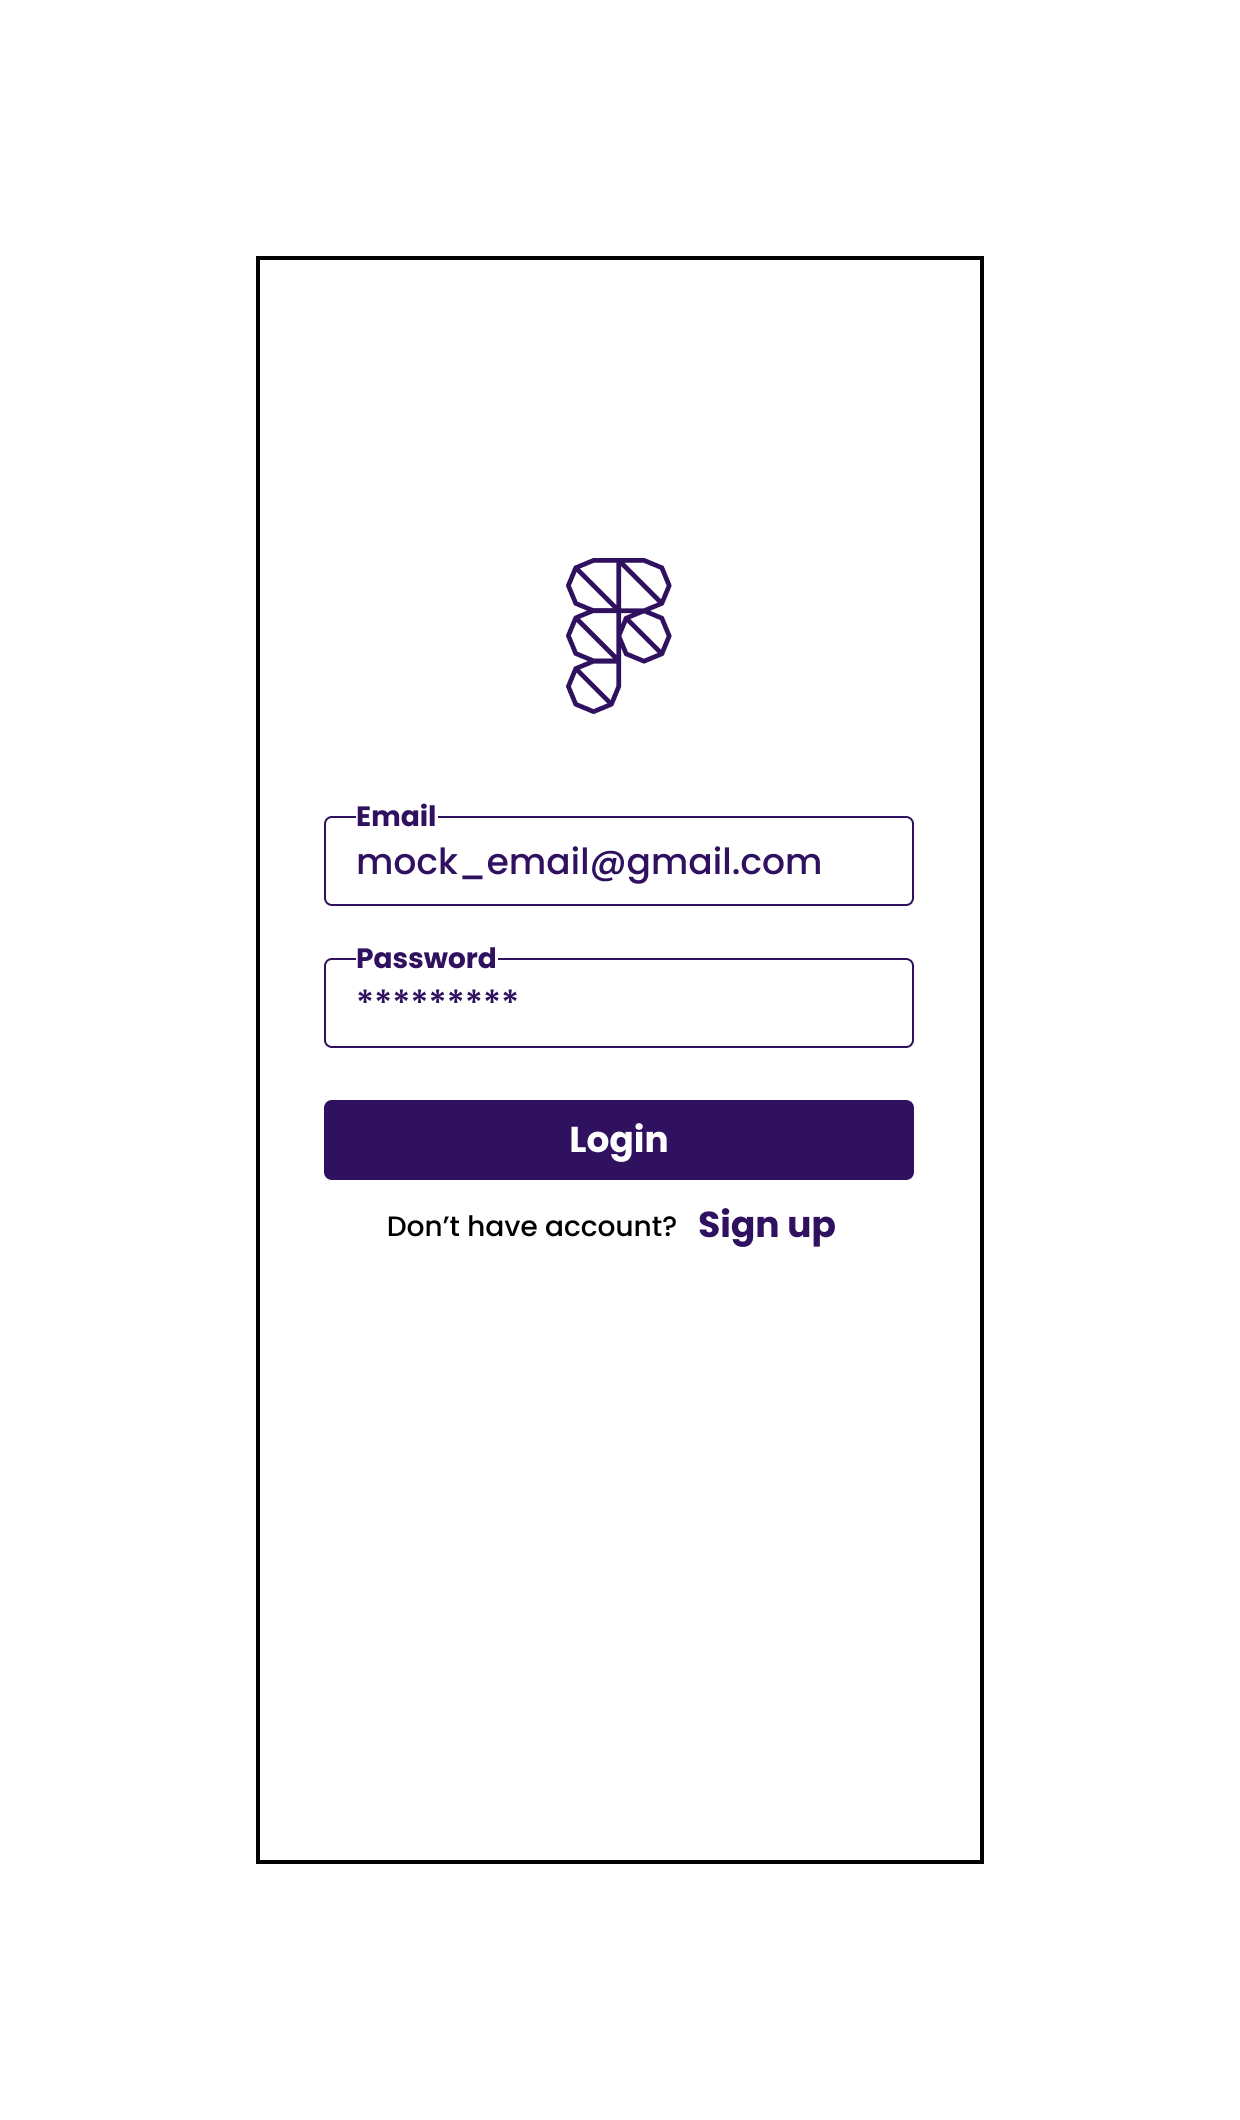
\includegraphics[width=0.57\textwidth]{images/DetailedDesign_LoginView.png}
    \caption{Detail Design: Login View}
    \label{fig:DetailedDesign_LoginView}
\end{figure}

\subsubsection{Sign Up View}
\begin{figure}[H]
    \centering
    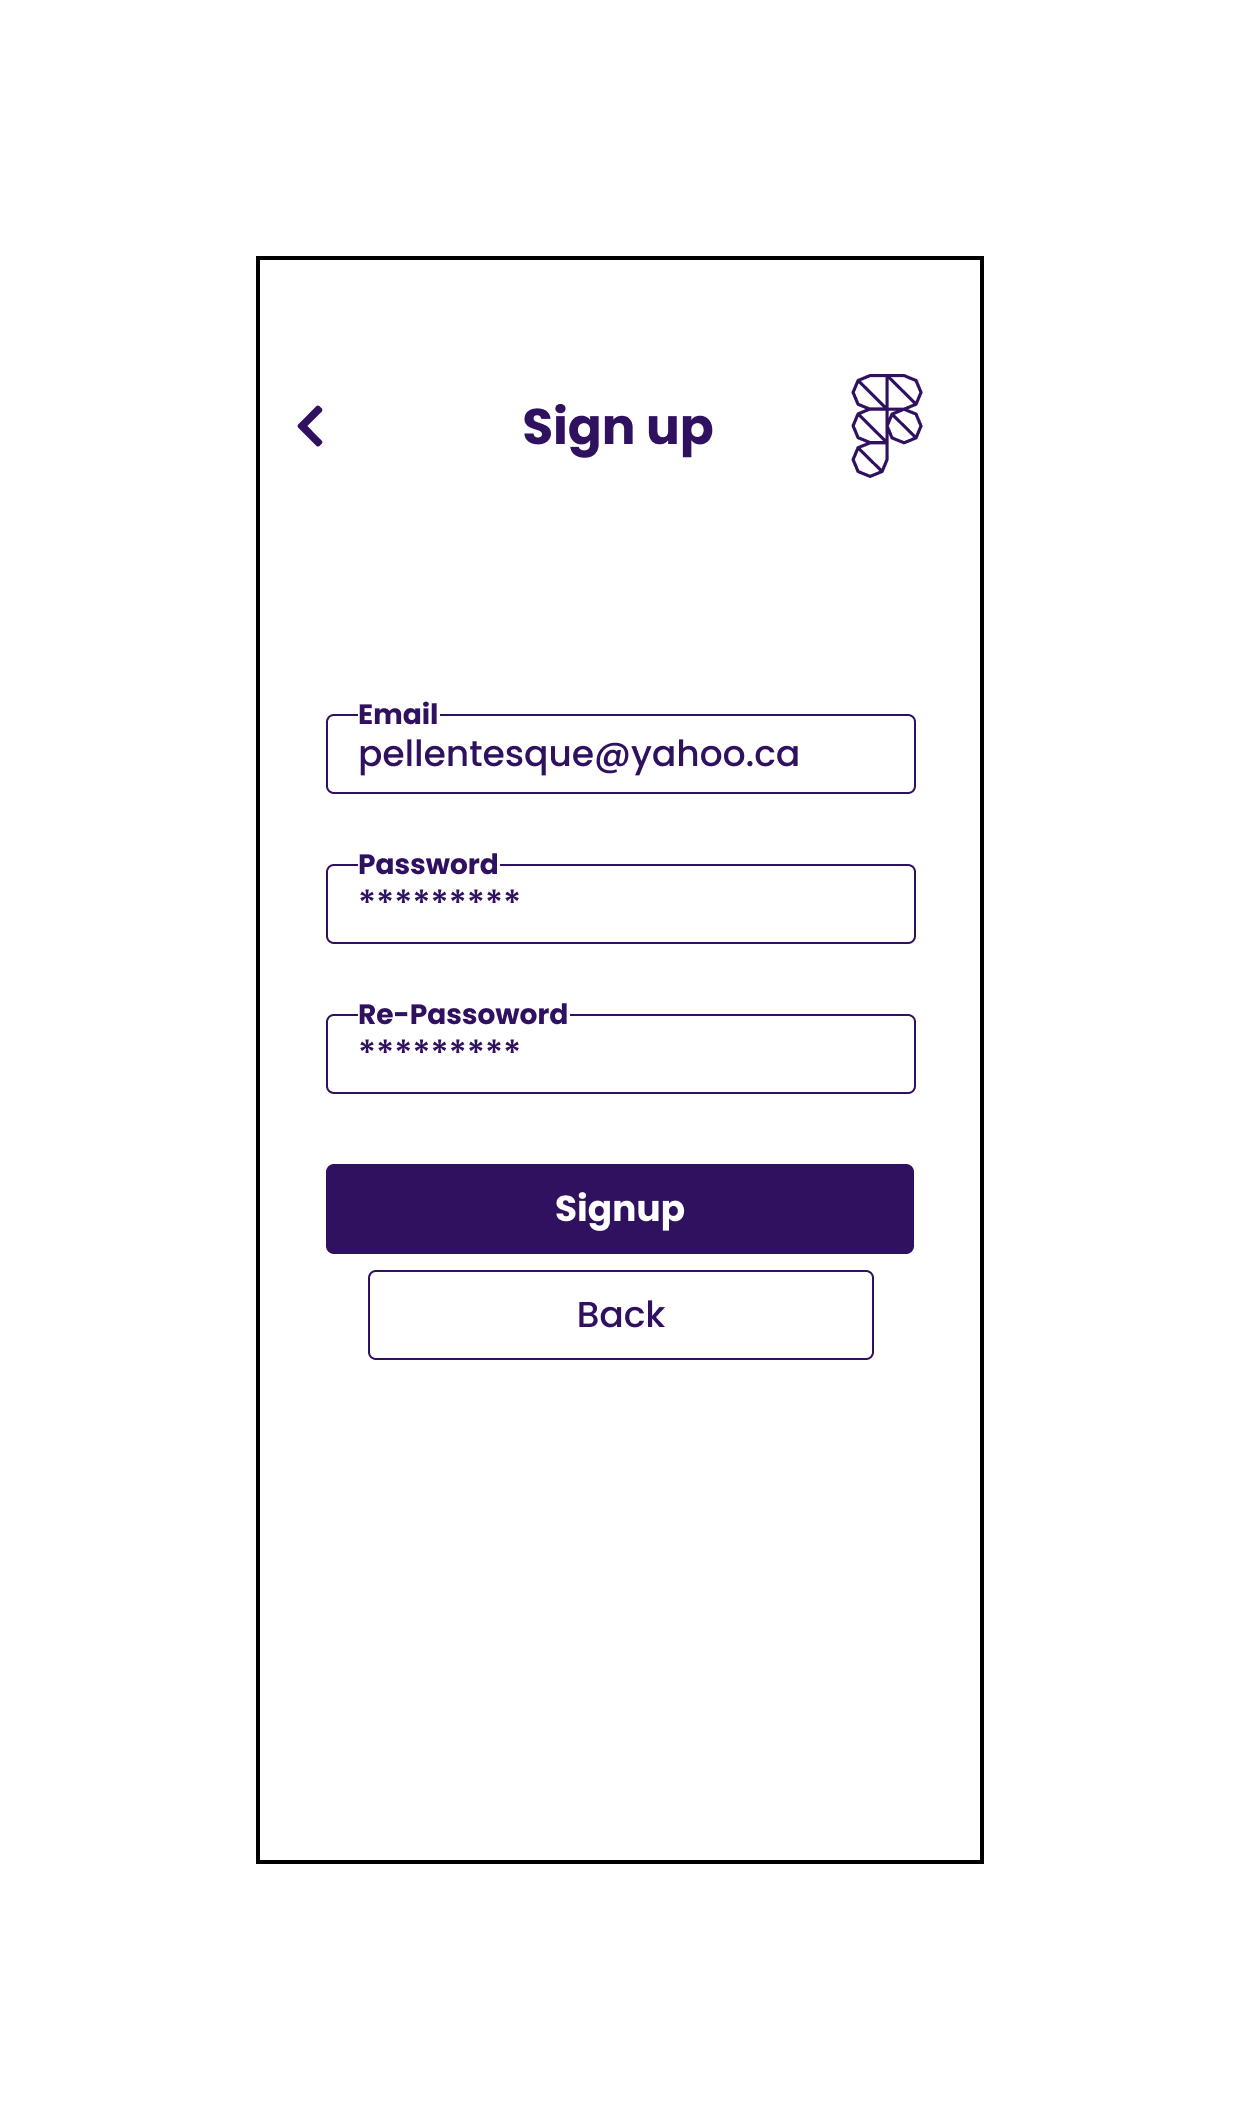
\includegraphics[width=0.57\textwidth]{images/DetailedDesign_SignUp.png}
    \caption{Detail Design: Sign Up View}
    \label{fig:DetailedDesign_SignUp}
\end{figure}

\subsection{Home View}

\begin{figure}[H]
    \centering
    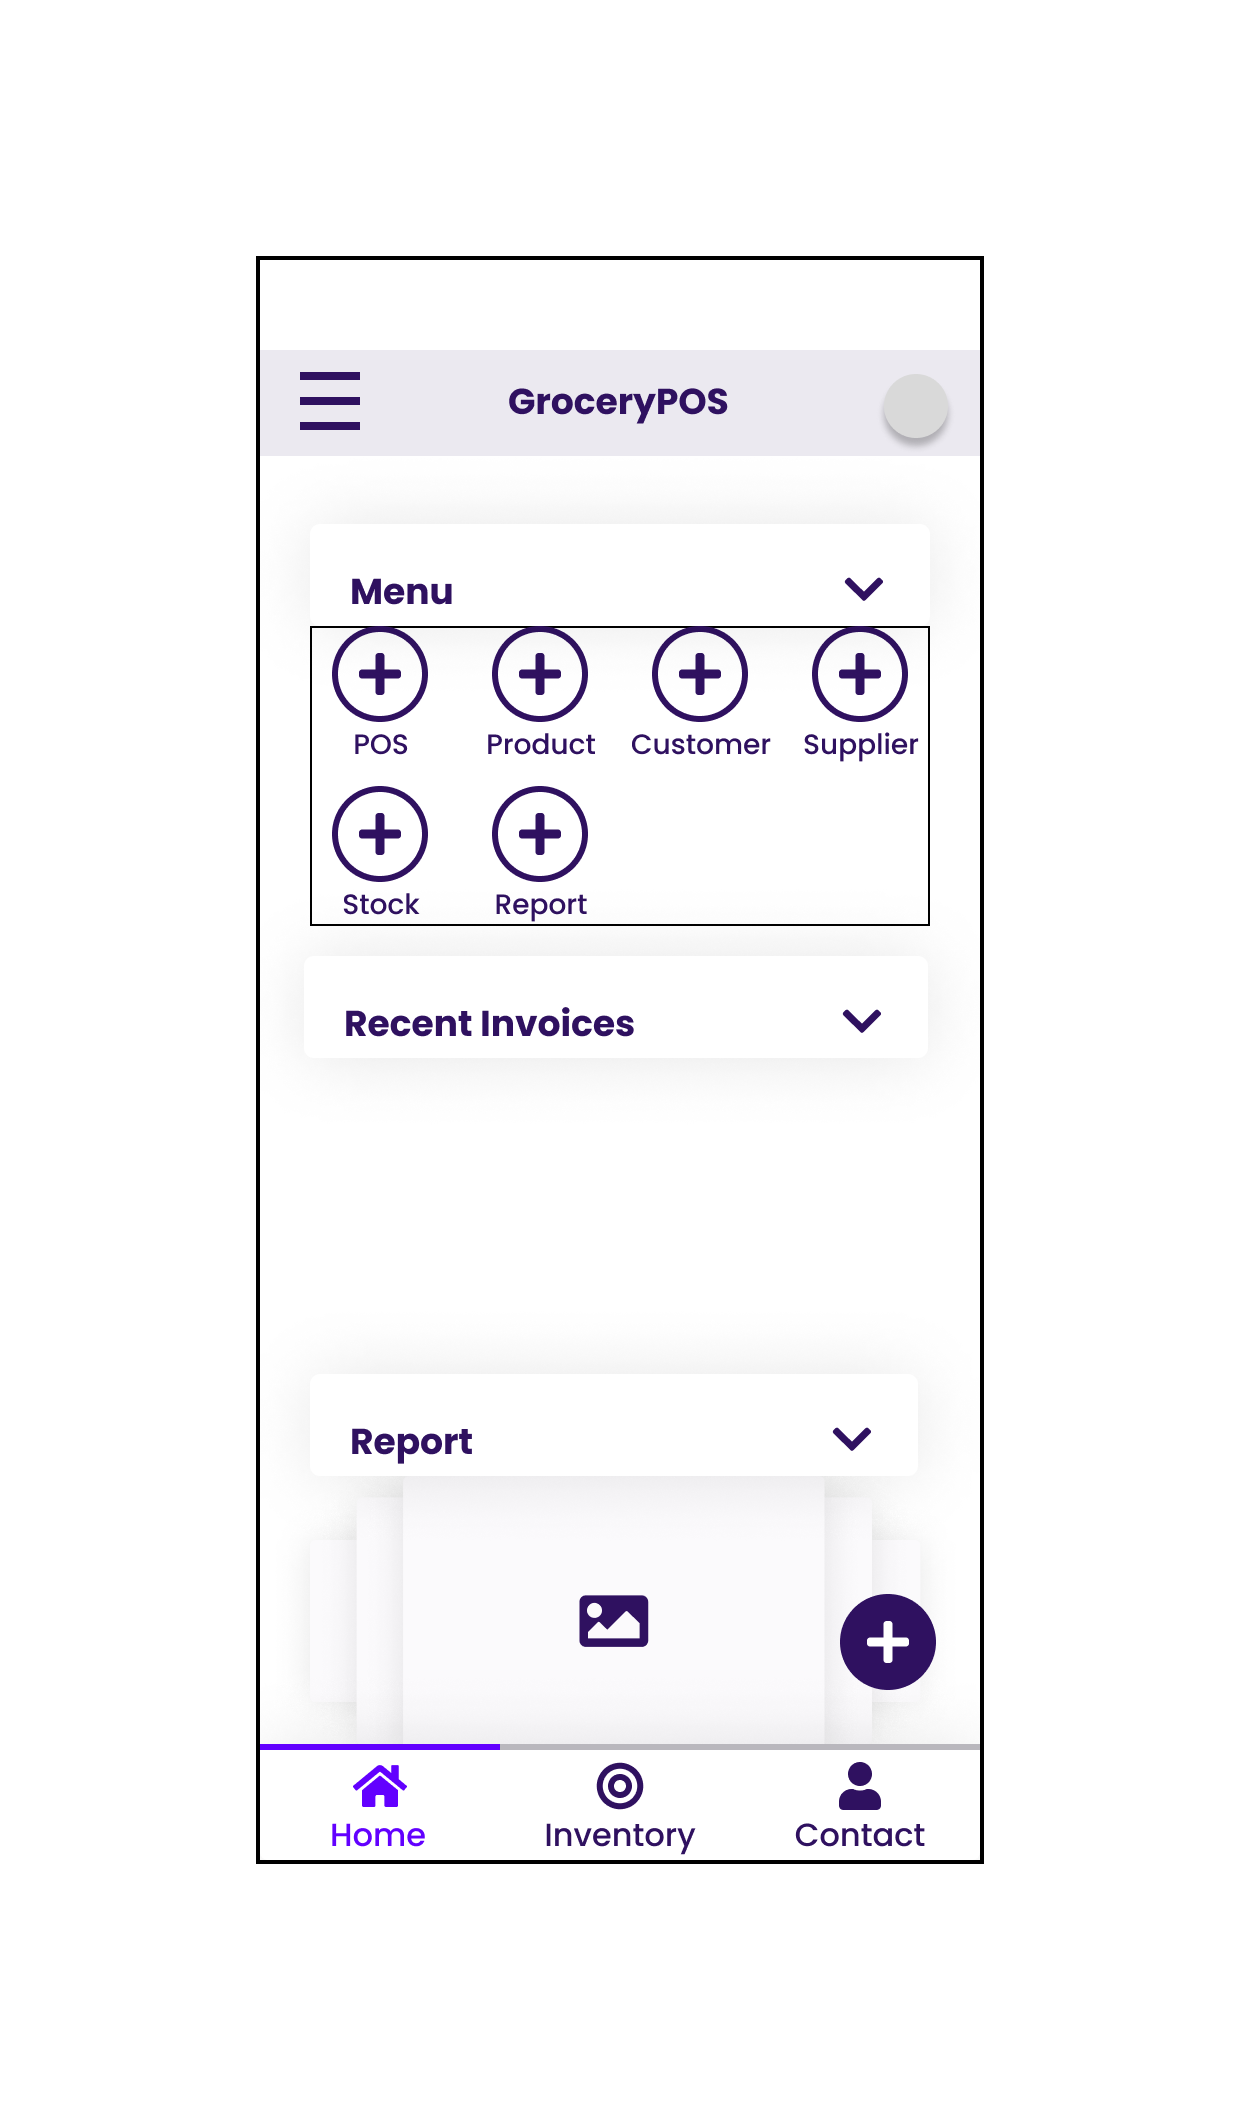
\includegraphics[width=0.57\textwidth]{images/DetailedDesign_Home.png}
    \caption{Detail Design: Home View}
    \label{fig:DetailedDesign_Home}
\end{figure}


\begin{figure}[H]
    \centering
    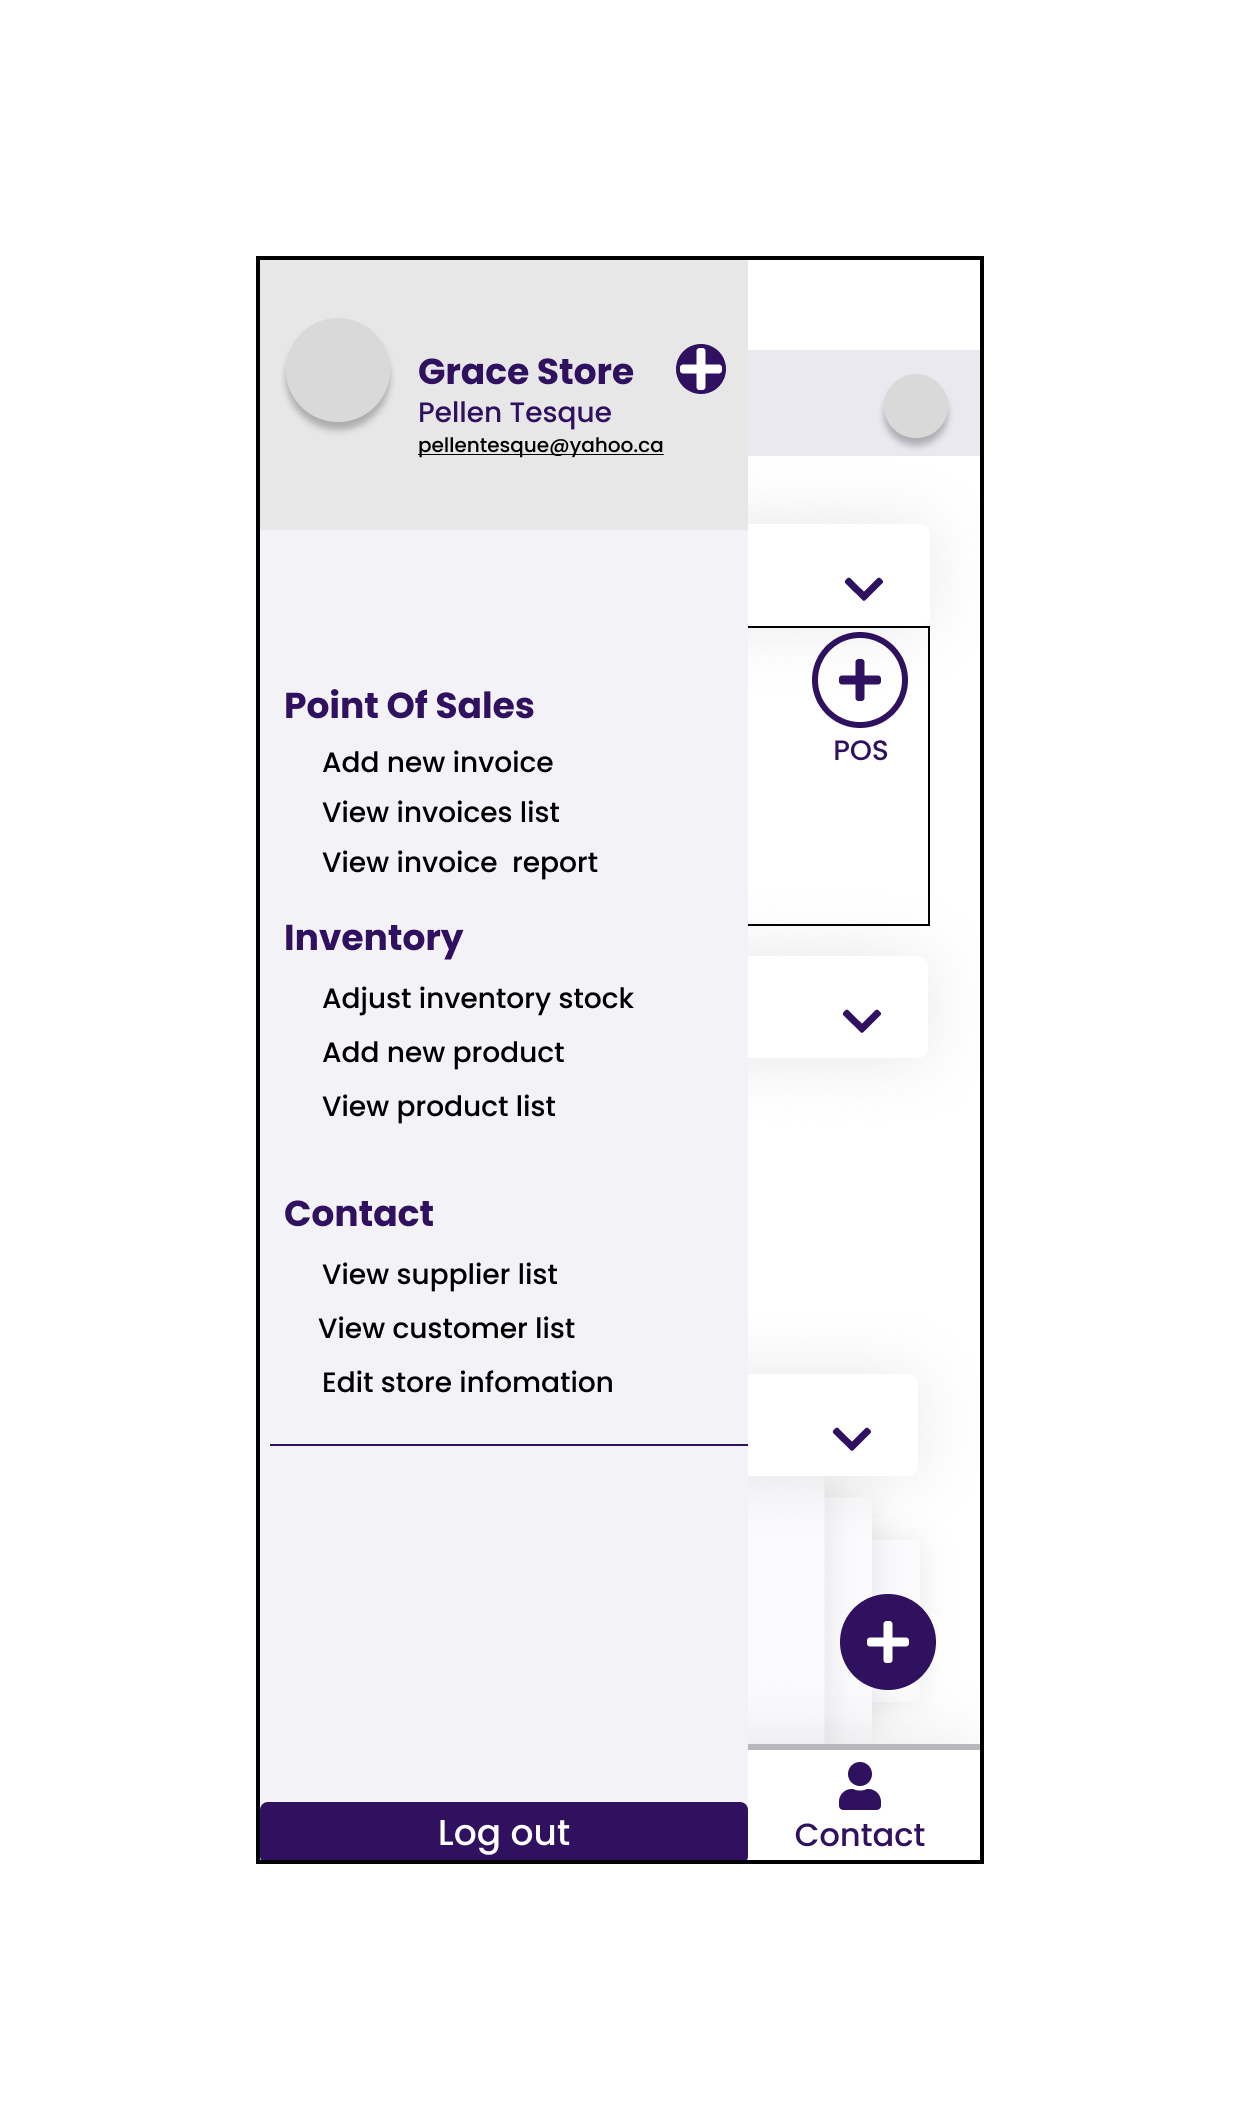
\includegraphics[width=0.57\textwidth]{images/DetailedDesign_Home_Navigate.png}
    \caption{Detail Design: Home View Side Menu}
    \label{fig:DetailedDesign_Home_Navigate}
\end{figure}

\subsection{User Profile View}

\begin{figure}[H]
    \centering
    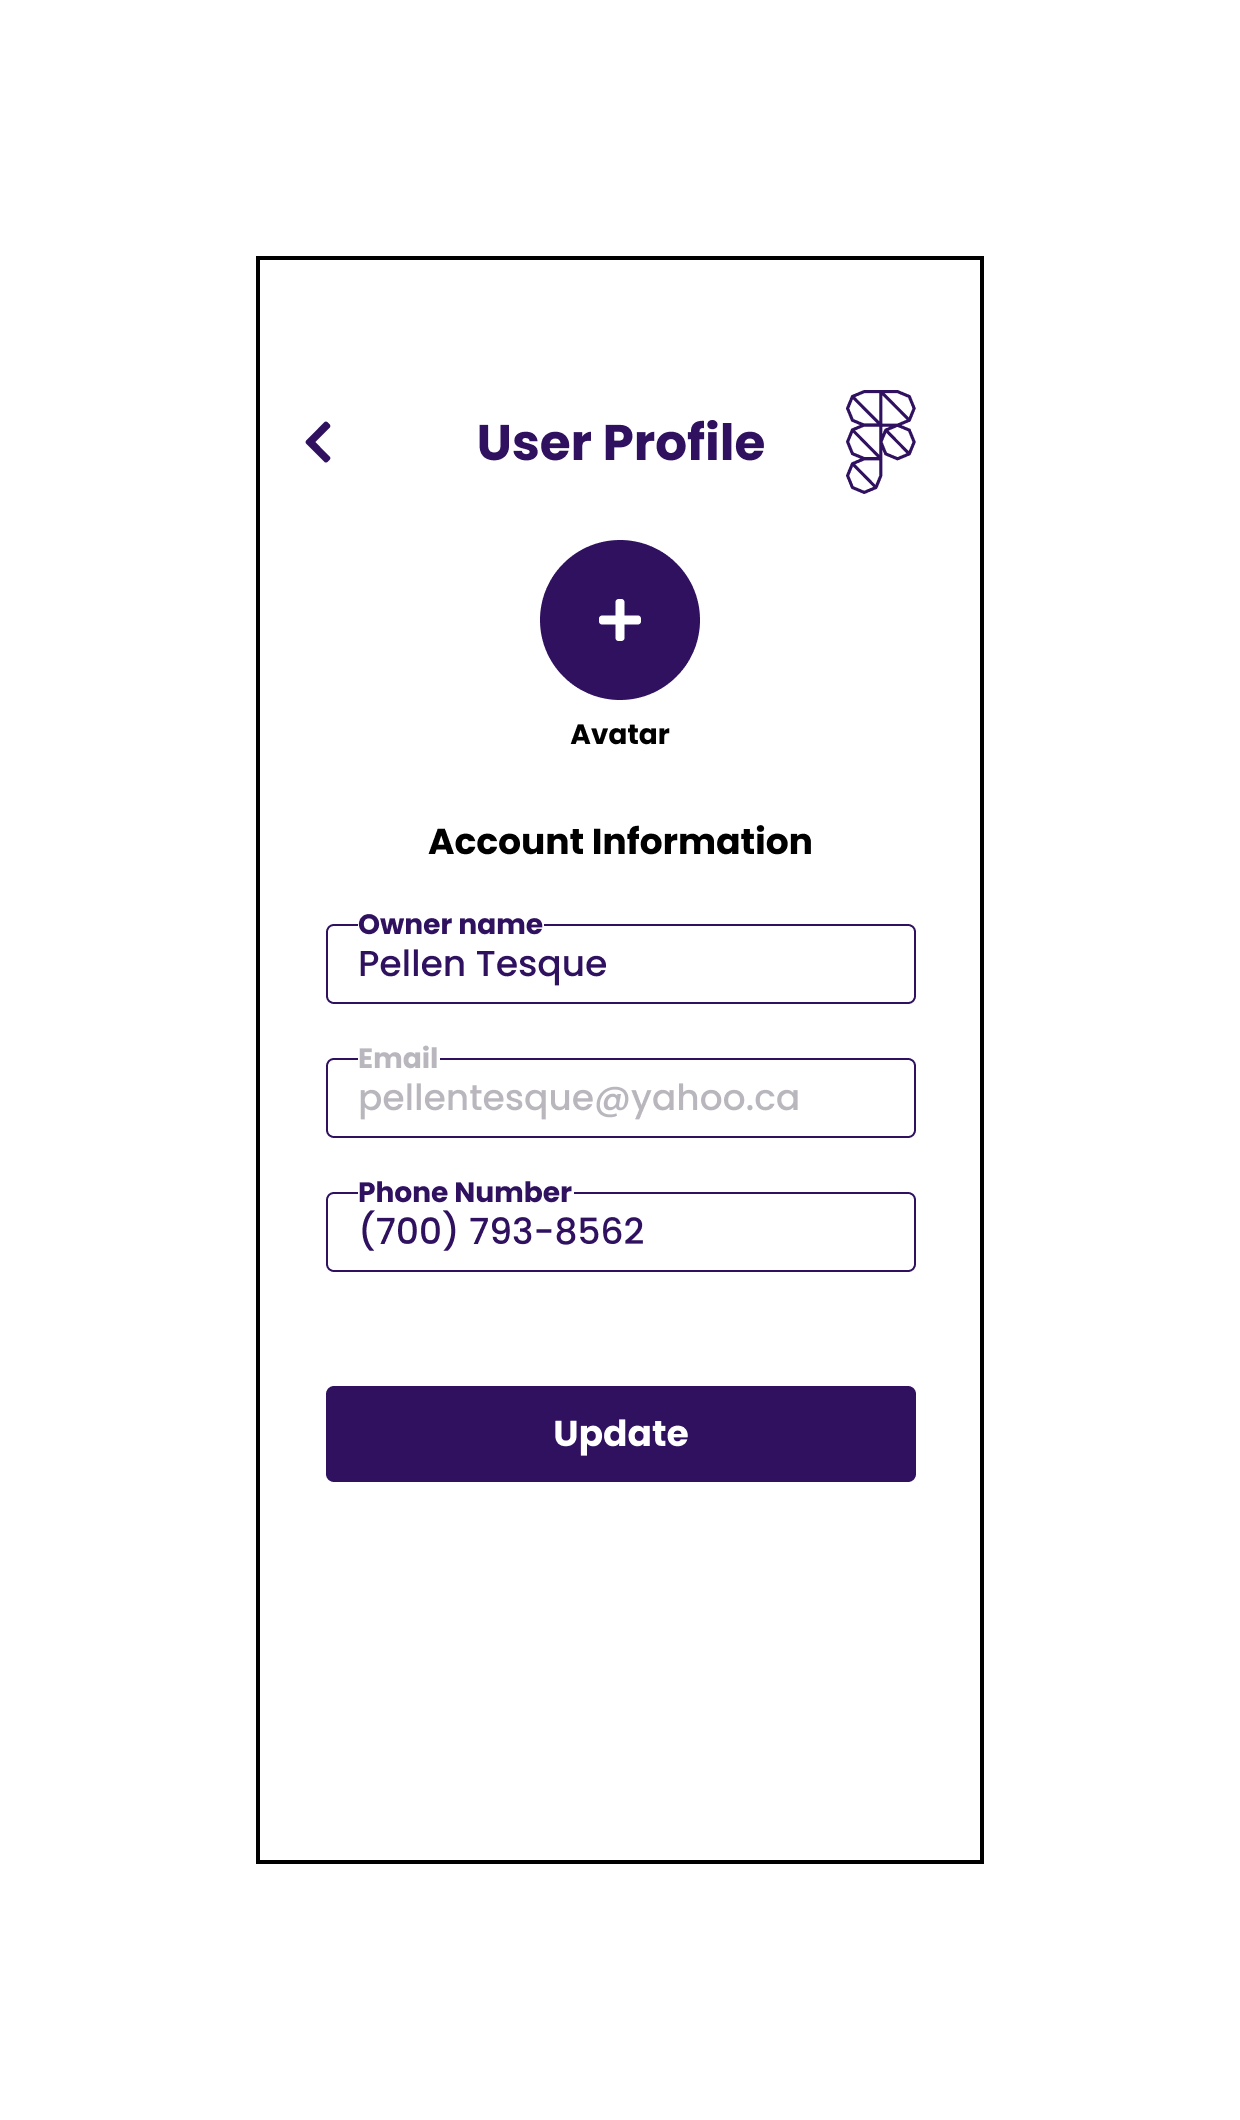
\includegraphics[width=0.57\textwidth]{images/DetailedDesign_UserProfile.png}
    \caption{Detail Design: User Profile View}
    \label{fig:DetailedDesign_UserProfile}
\end{figure}

\subsection{Store Profile View}

\begin{figure}[H]
    \centering
    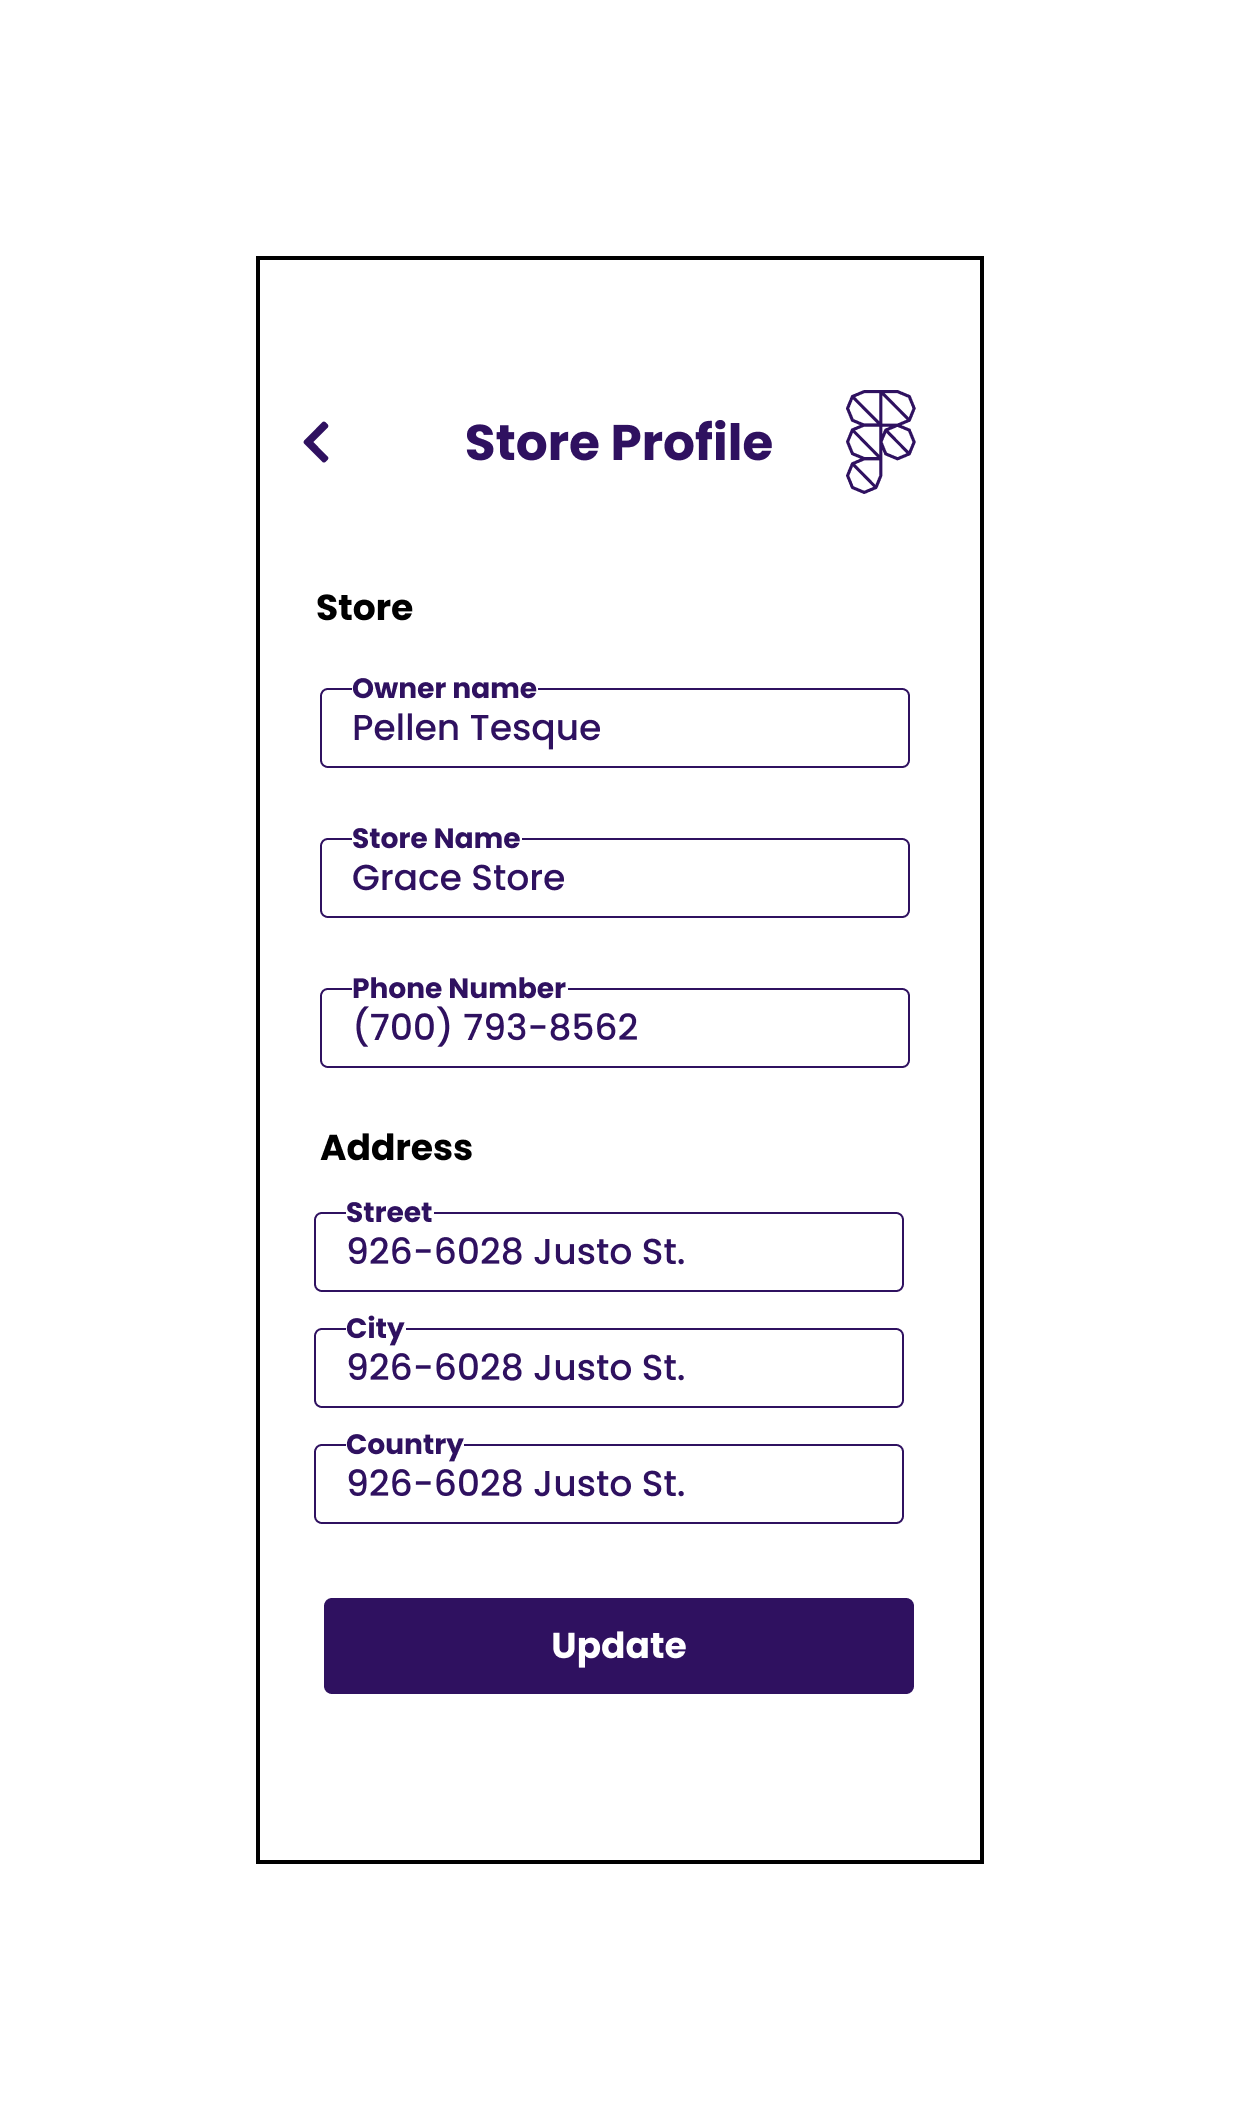
\includegraphics[width=0.57\textwidth]{images/DetailedDesign_StoreProfile.png}
    \caption{Detail Design: Store Profile View}
    \label{fig:DetailedDesign_StoreProfile}
\end{figure}

\subsection{Contacts}
\subsubsection{Supplier View}

\begin{figure}[H]
    \centering
    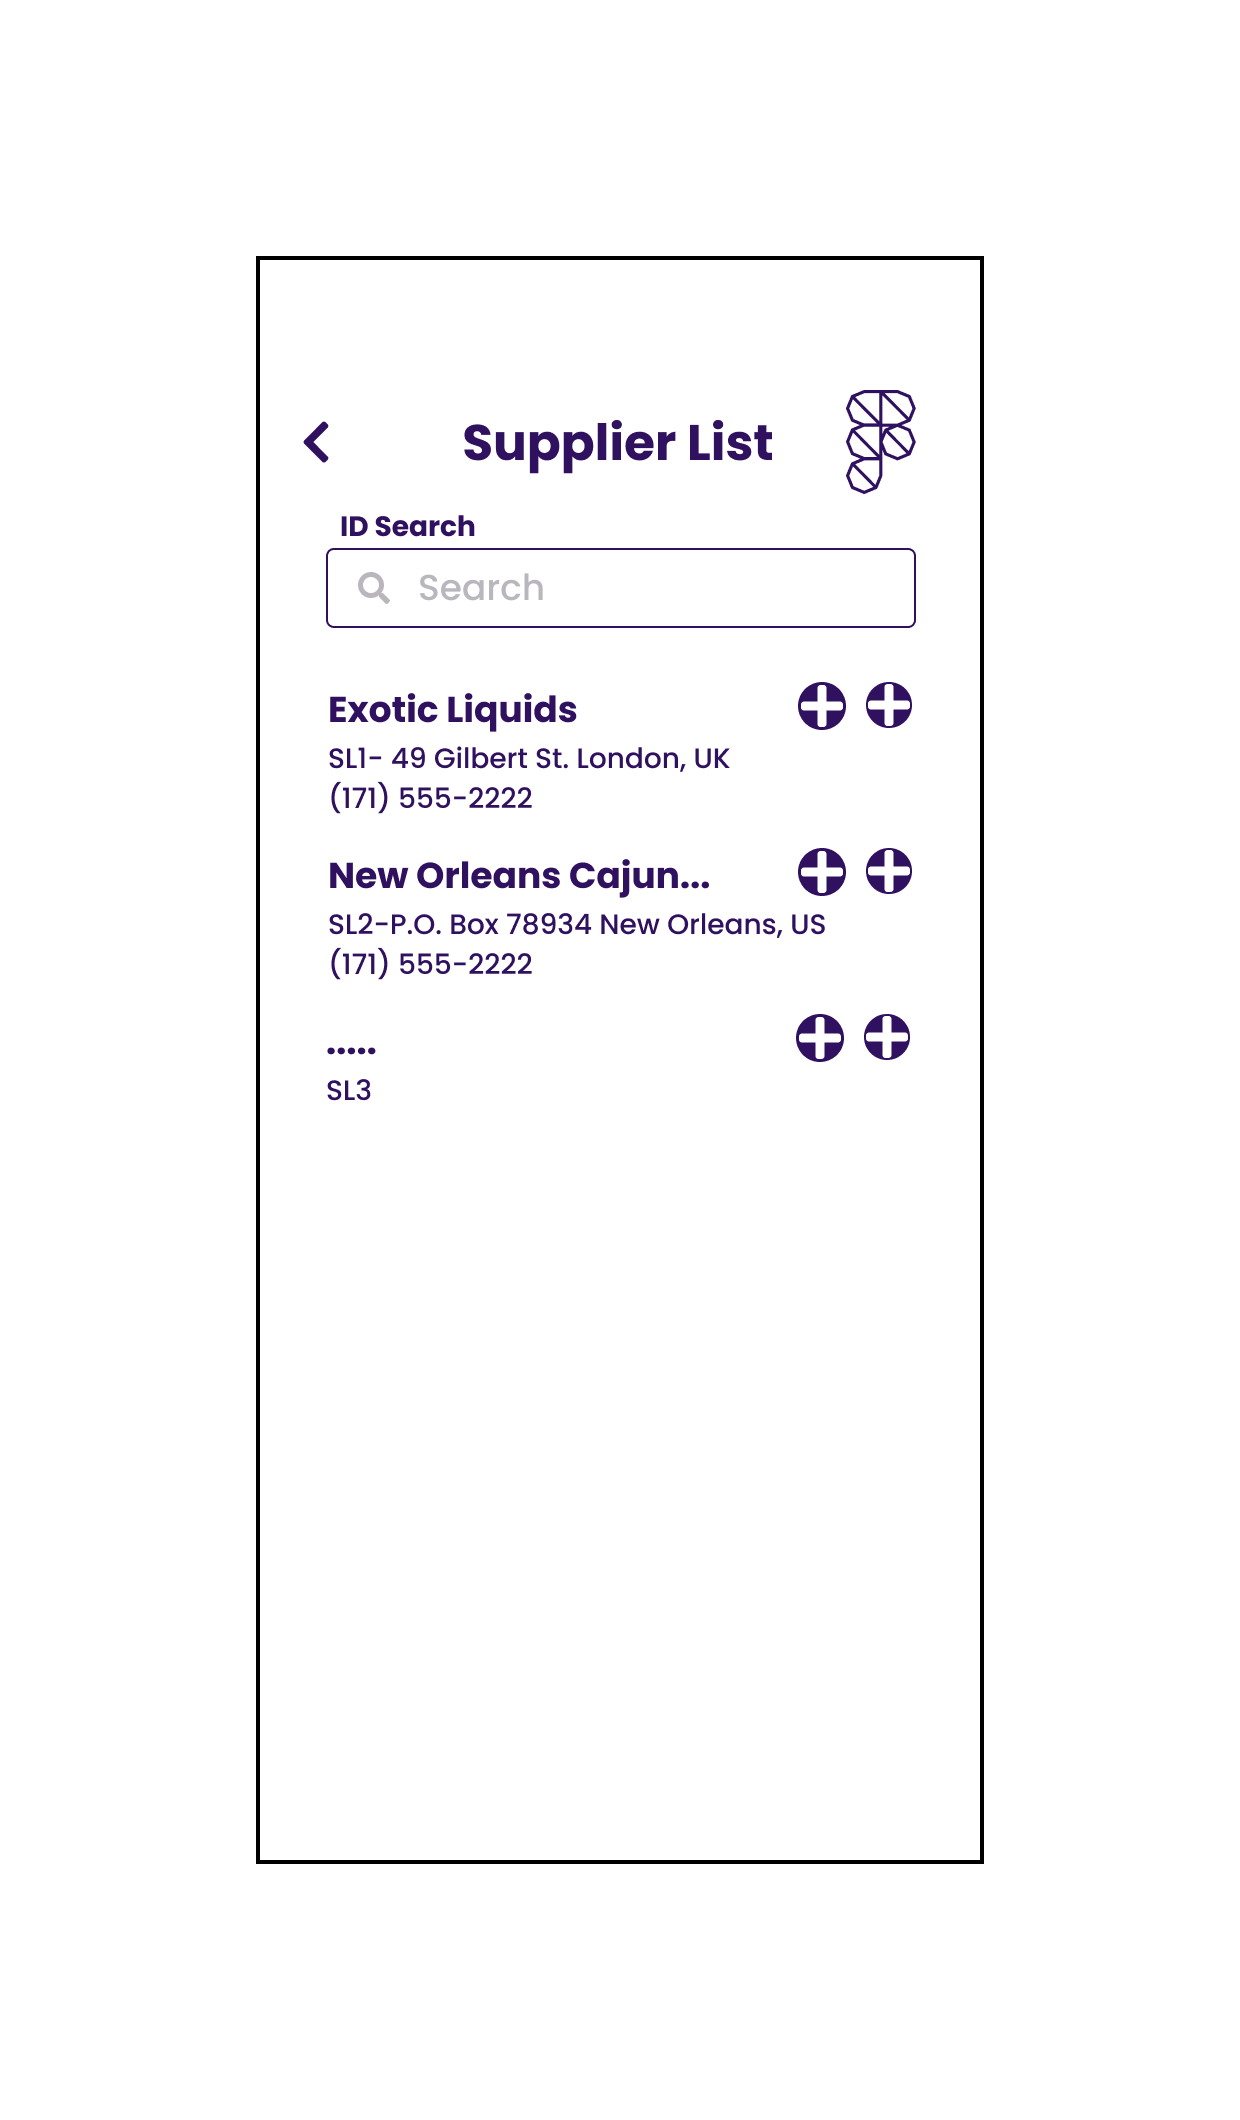
\includegraphics[width=0.57\textwidth]{images/DetailedDesign_Supplier_List.png}
    \caption{Detail Design: Supplier List View}
    \label{fig:DetailedDesign_Supplier_List}
\end{figure}

\begin{figure}[H]
    \centering
    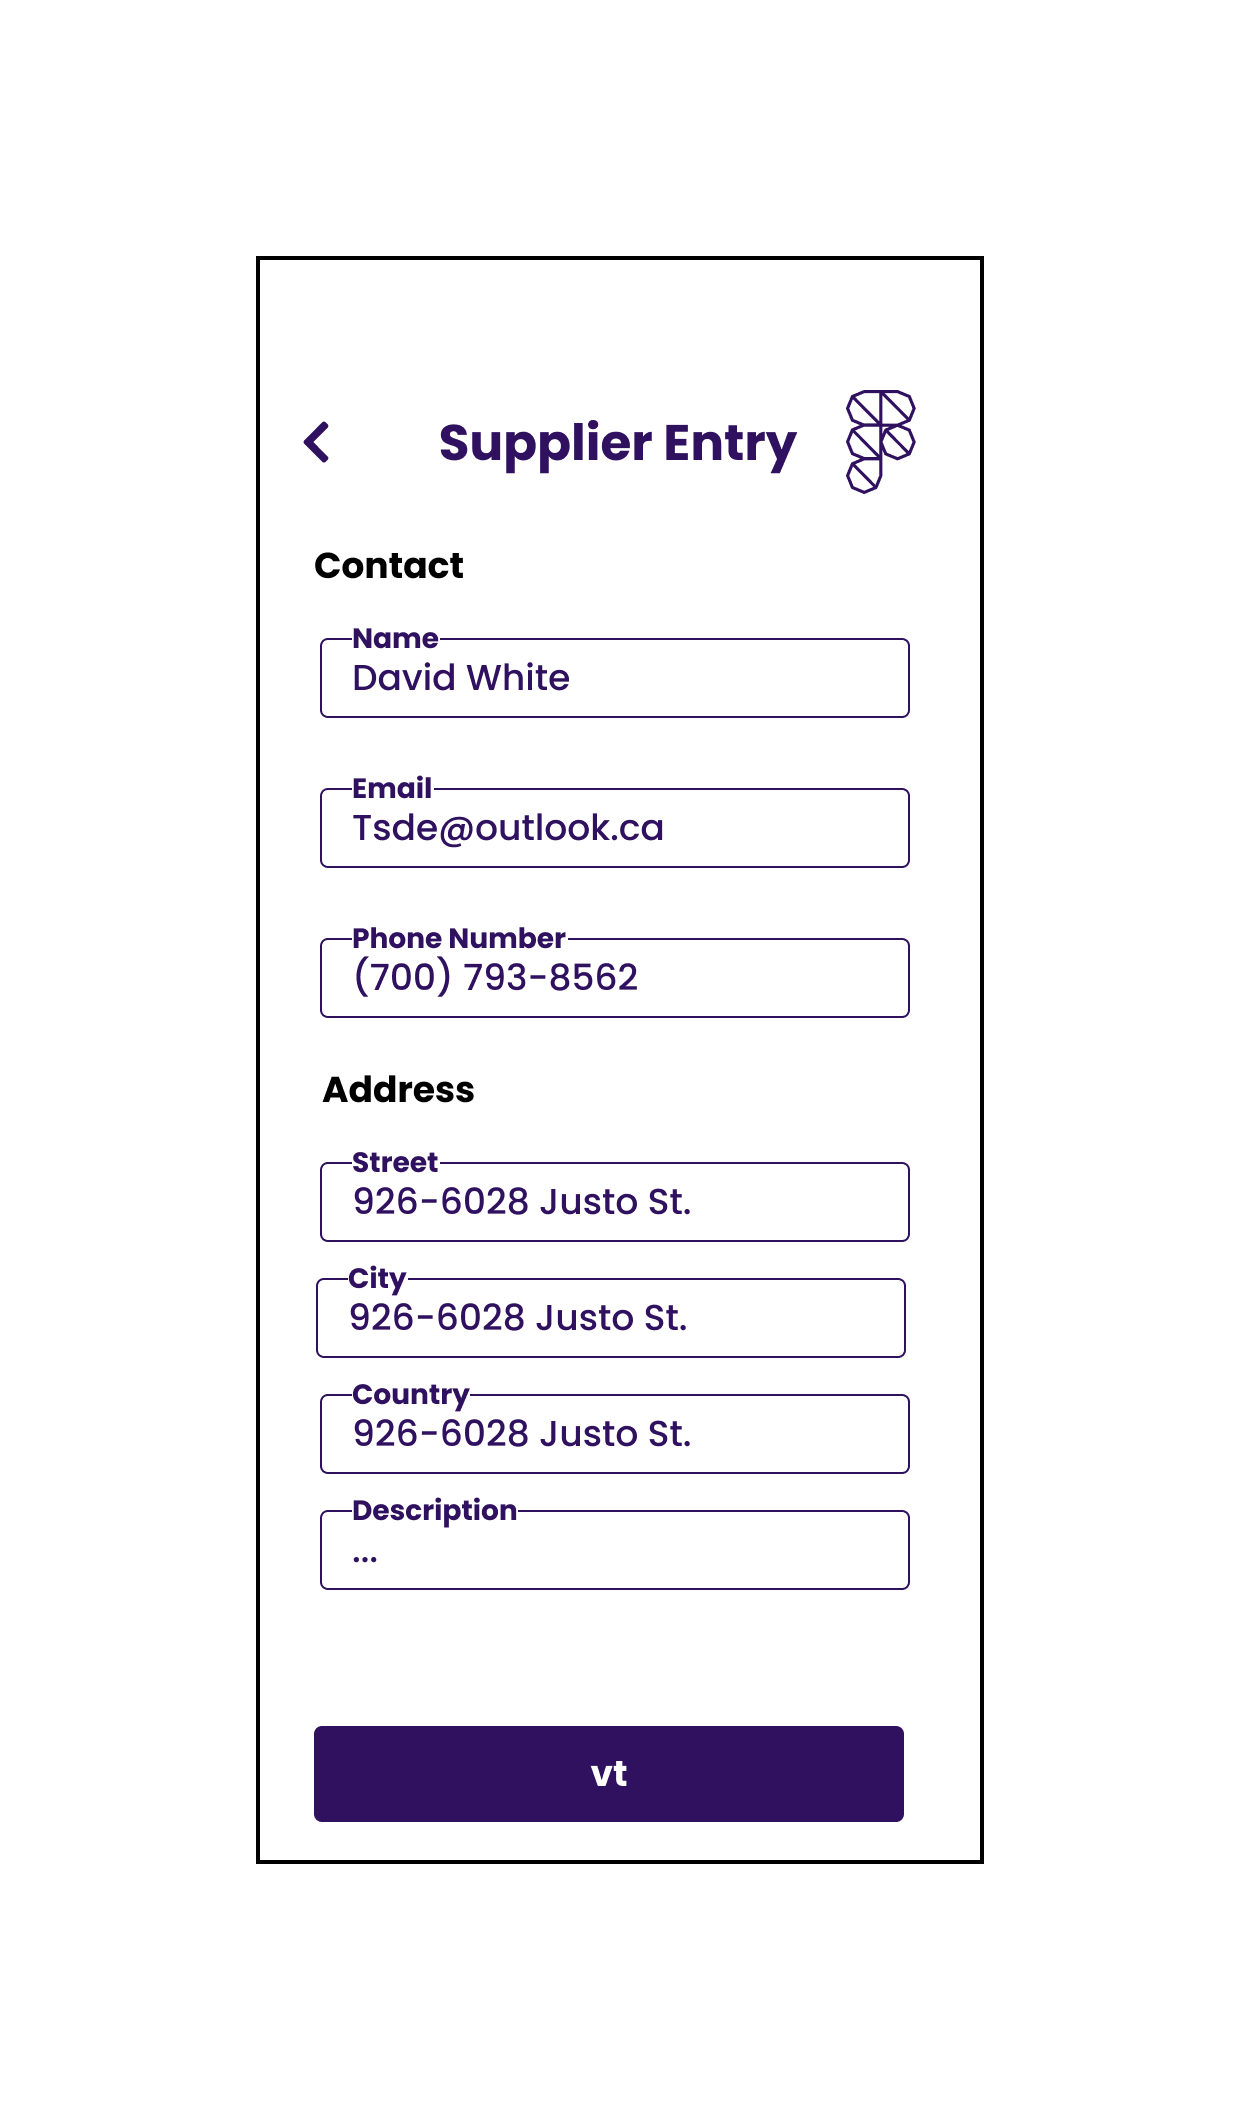
\includegraphics[width=0.57\textwidth]{images/DetailedDesign_Supplier_Entry.png}
    \caption{Detail Design: Supplier Entry View}
    \label{fig:DetailedDesign_Supplier_Entry}
\end{figure}

\subsubsection{Customer View}

\begin{figure}[H]
    \centering
    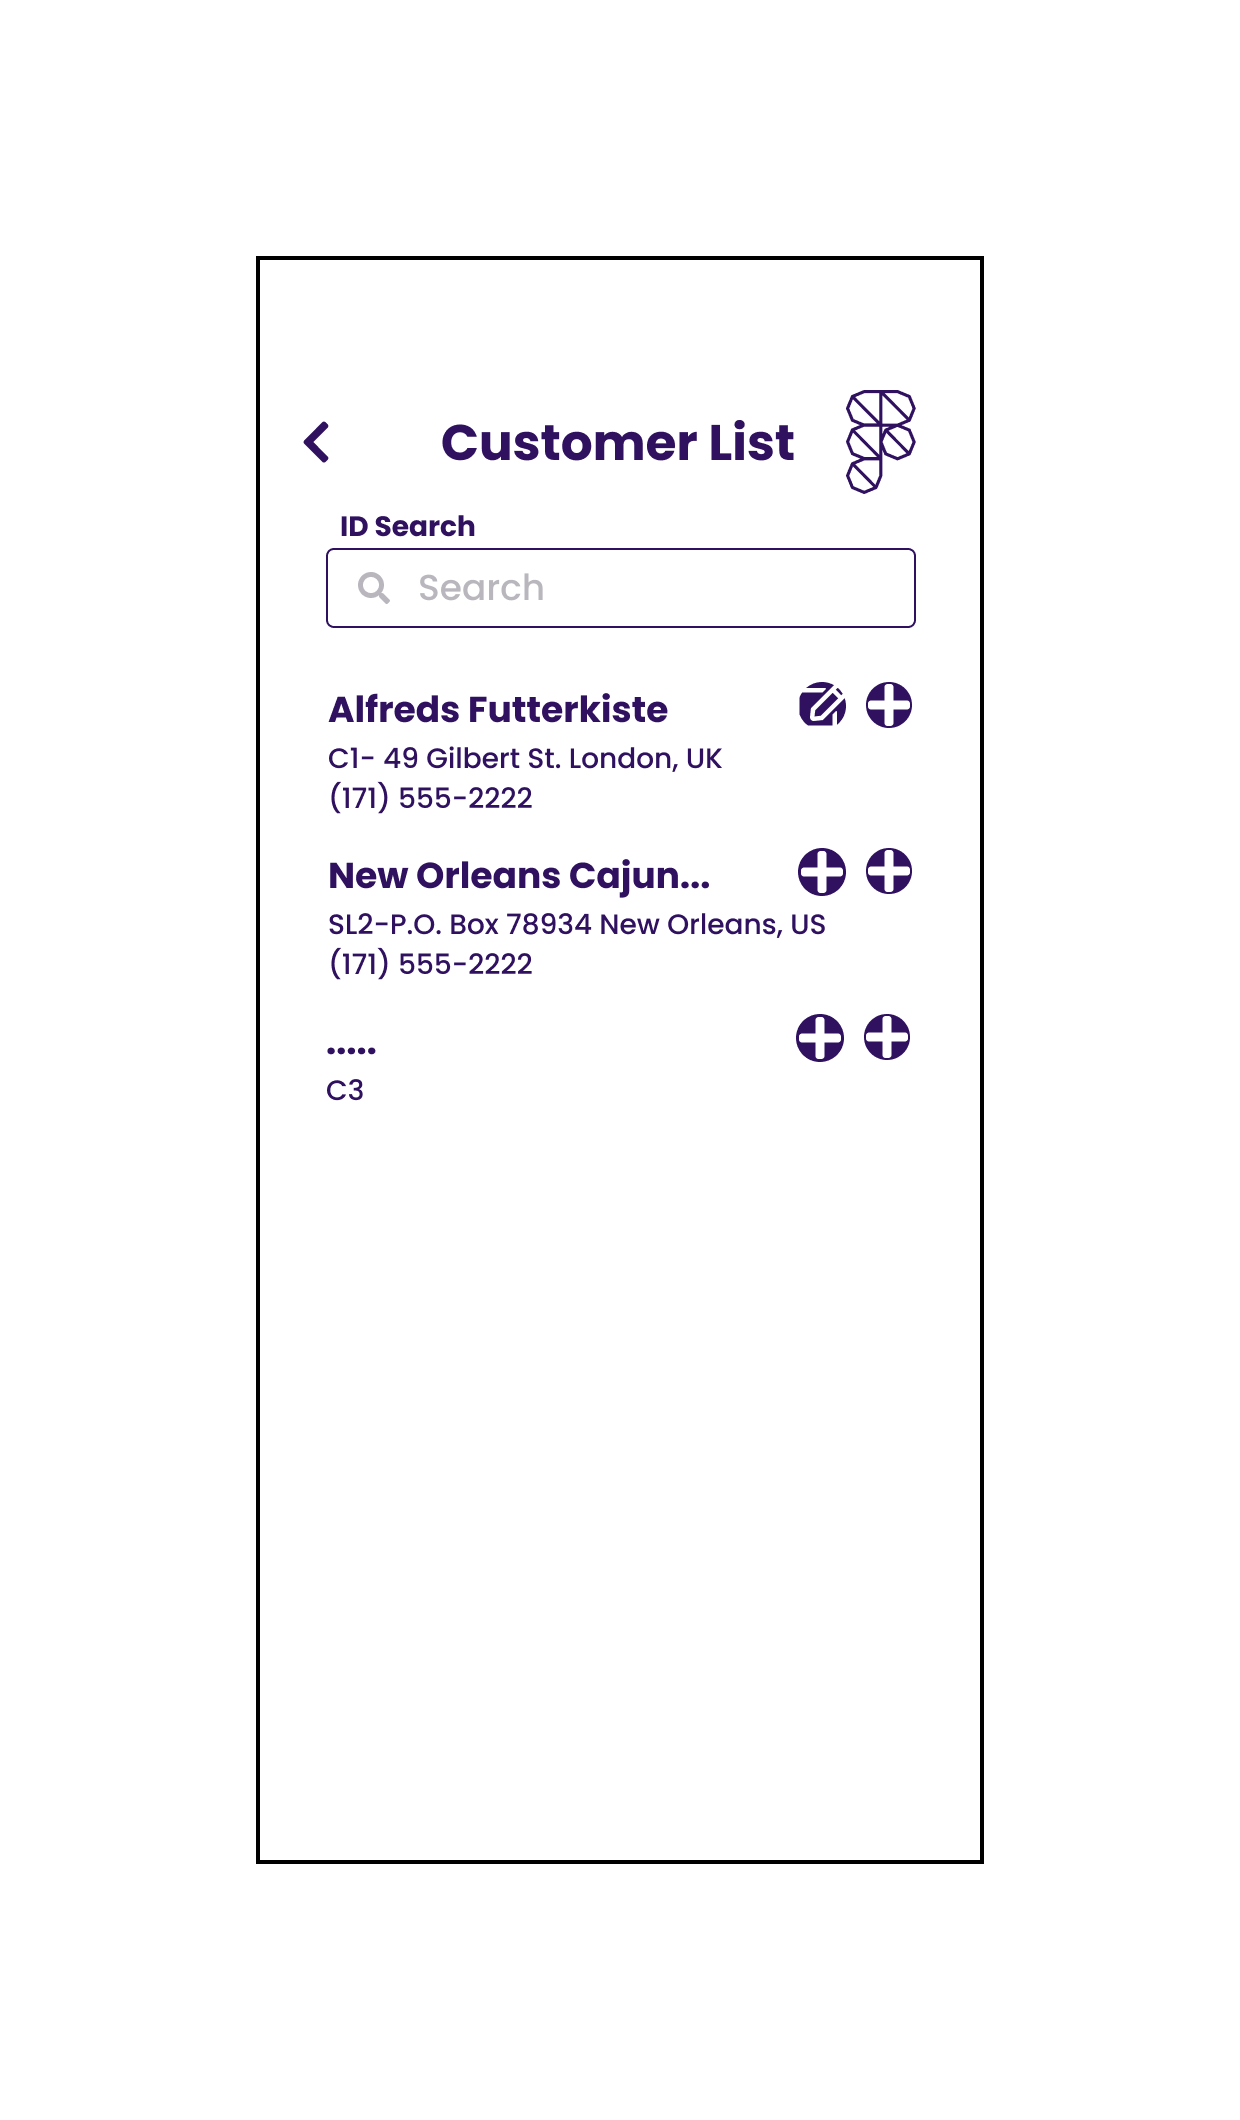
\includegraphics[width=0.57\textwidth]{images/DetailedDesign_Customer_List.png}
    \caption{Detail Design: Customer List View}
    \label{fig:DetailedDesign_Customer_List}
\end{figure}

\begin{figure}[H]
    \centering
    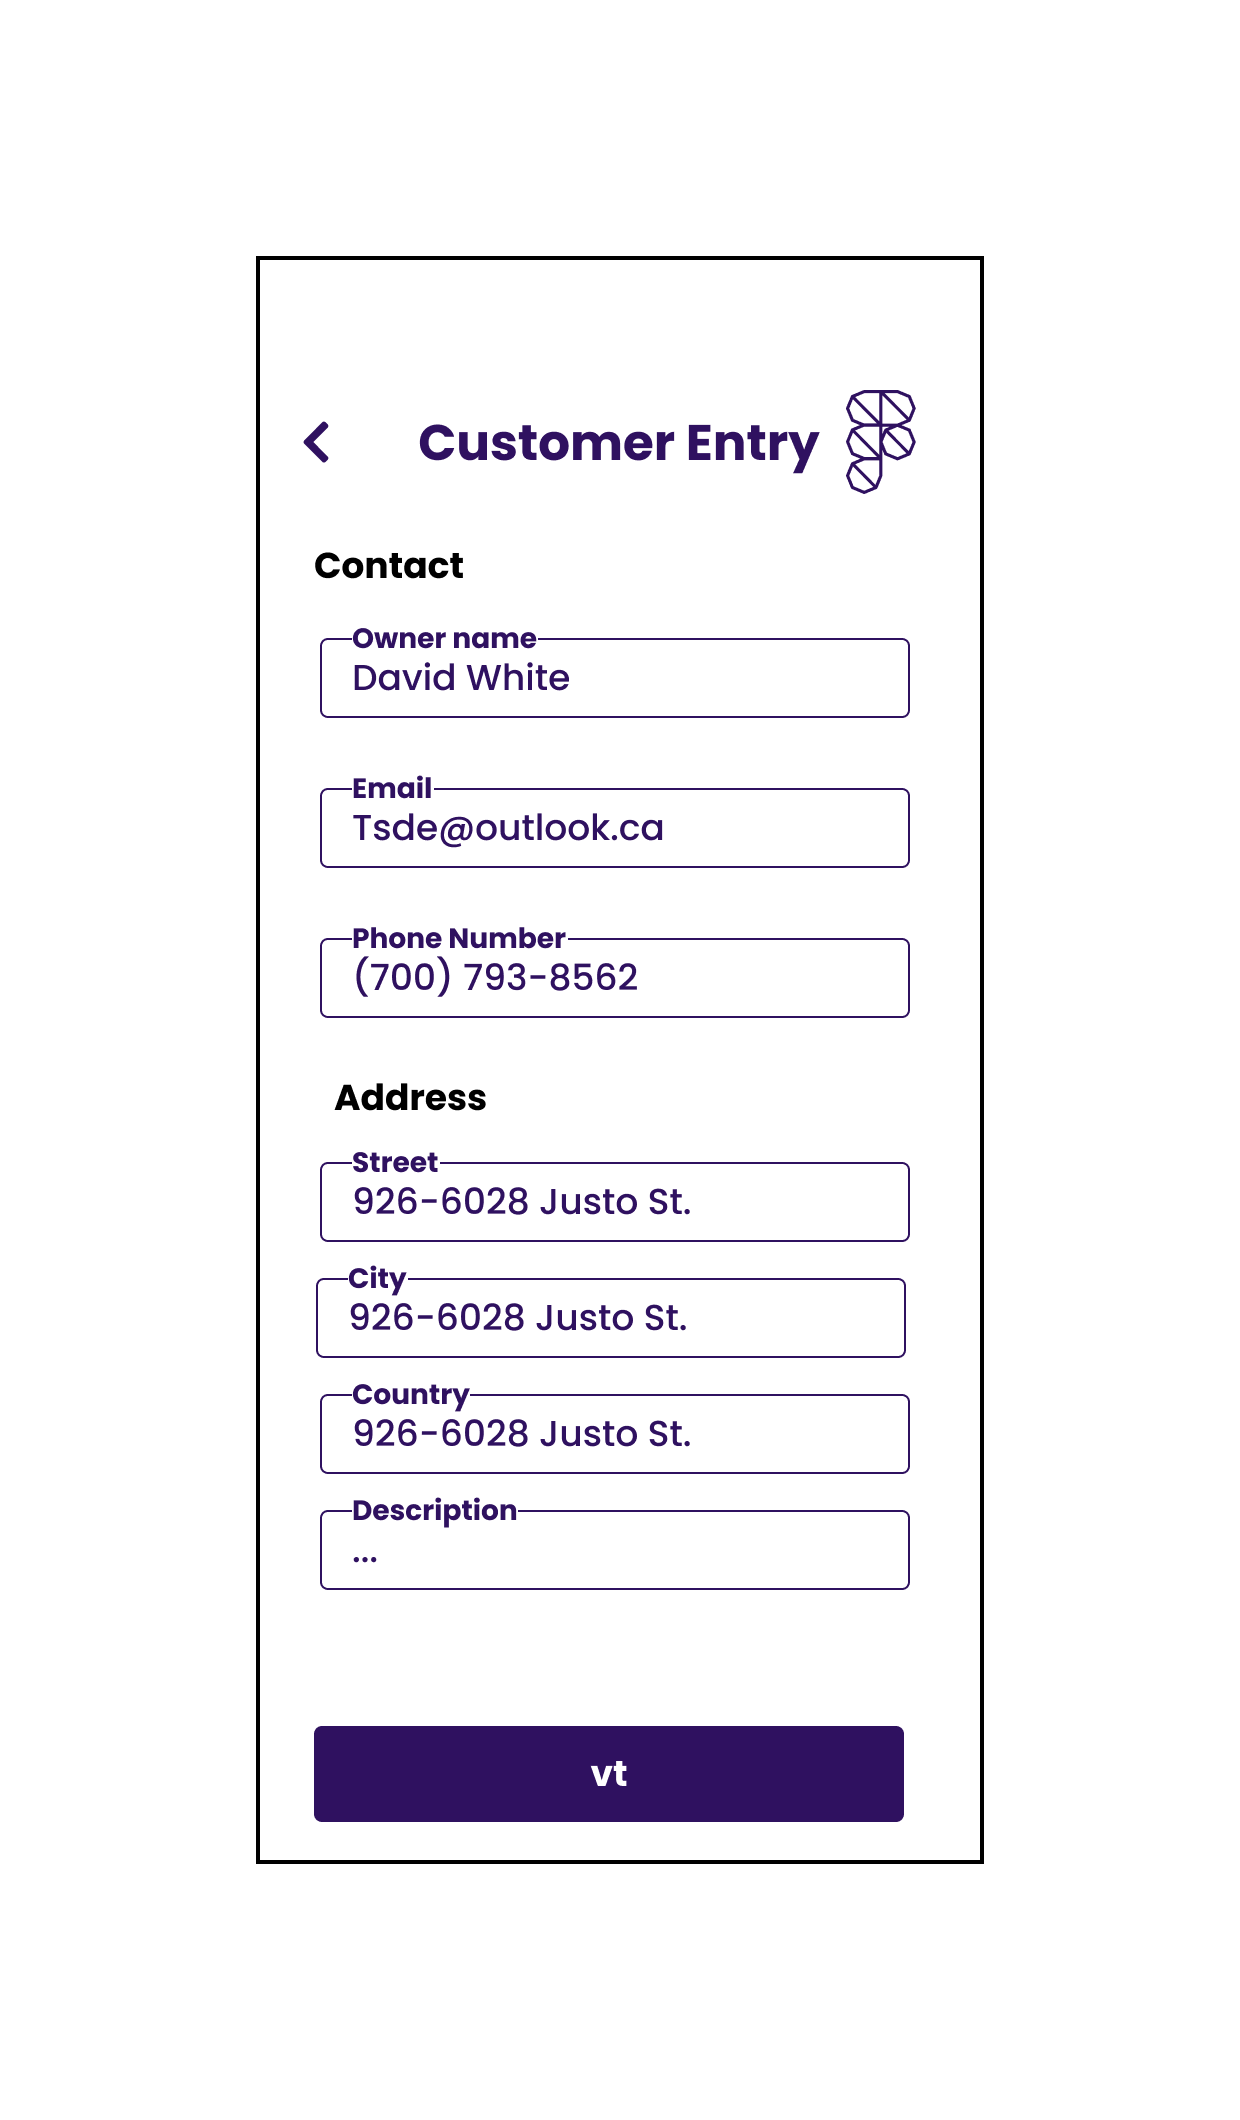
\includegraphics[width=0.57\textwidth]{images/DetailedDesign_Customer_Entry.png}
    \caption{Detail Design: Customer Entry View}
    \label{fig:DetailedDesign_Customer_Entry}
\end{figure}


\subsection{Inventory View}
\subsubsection{Category View}

\begin{figure}[H]
    \centering
    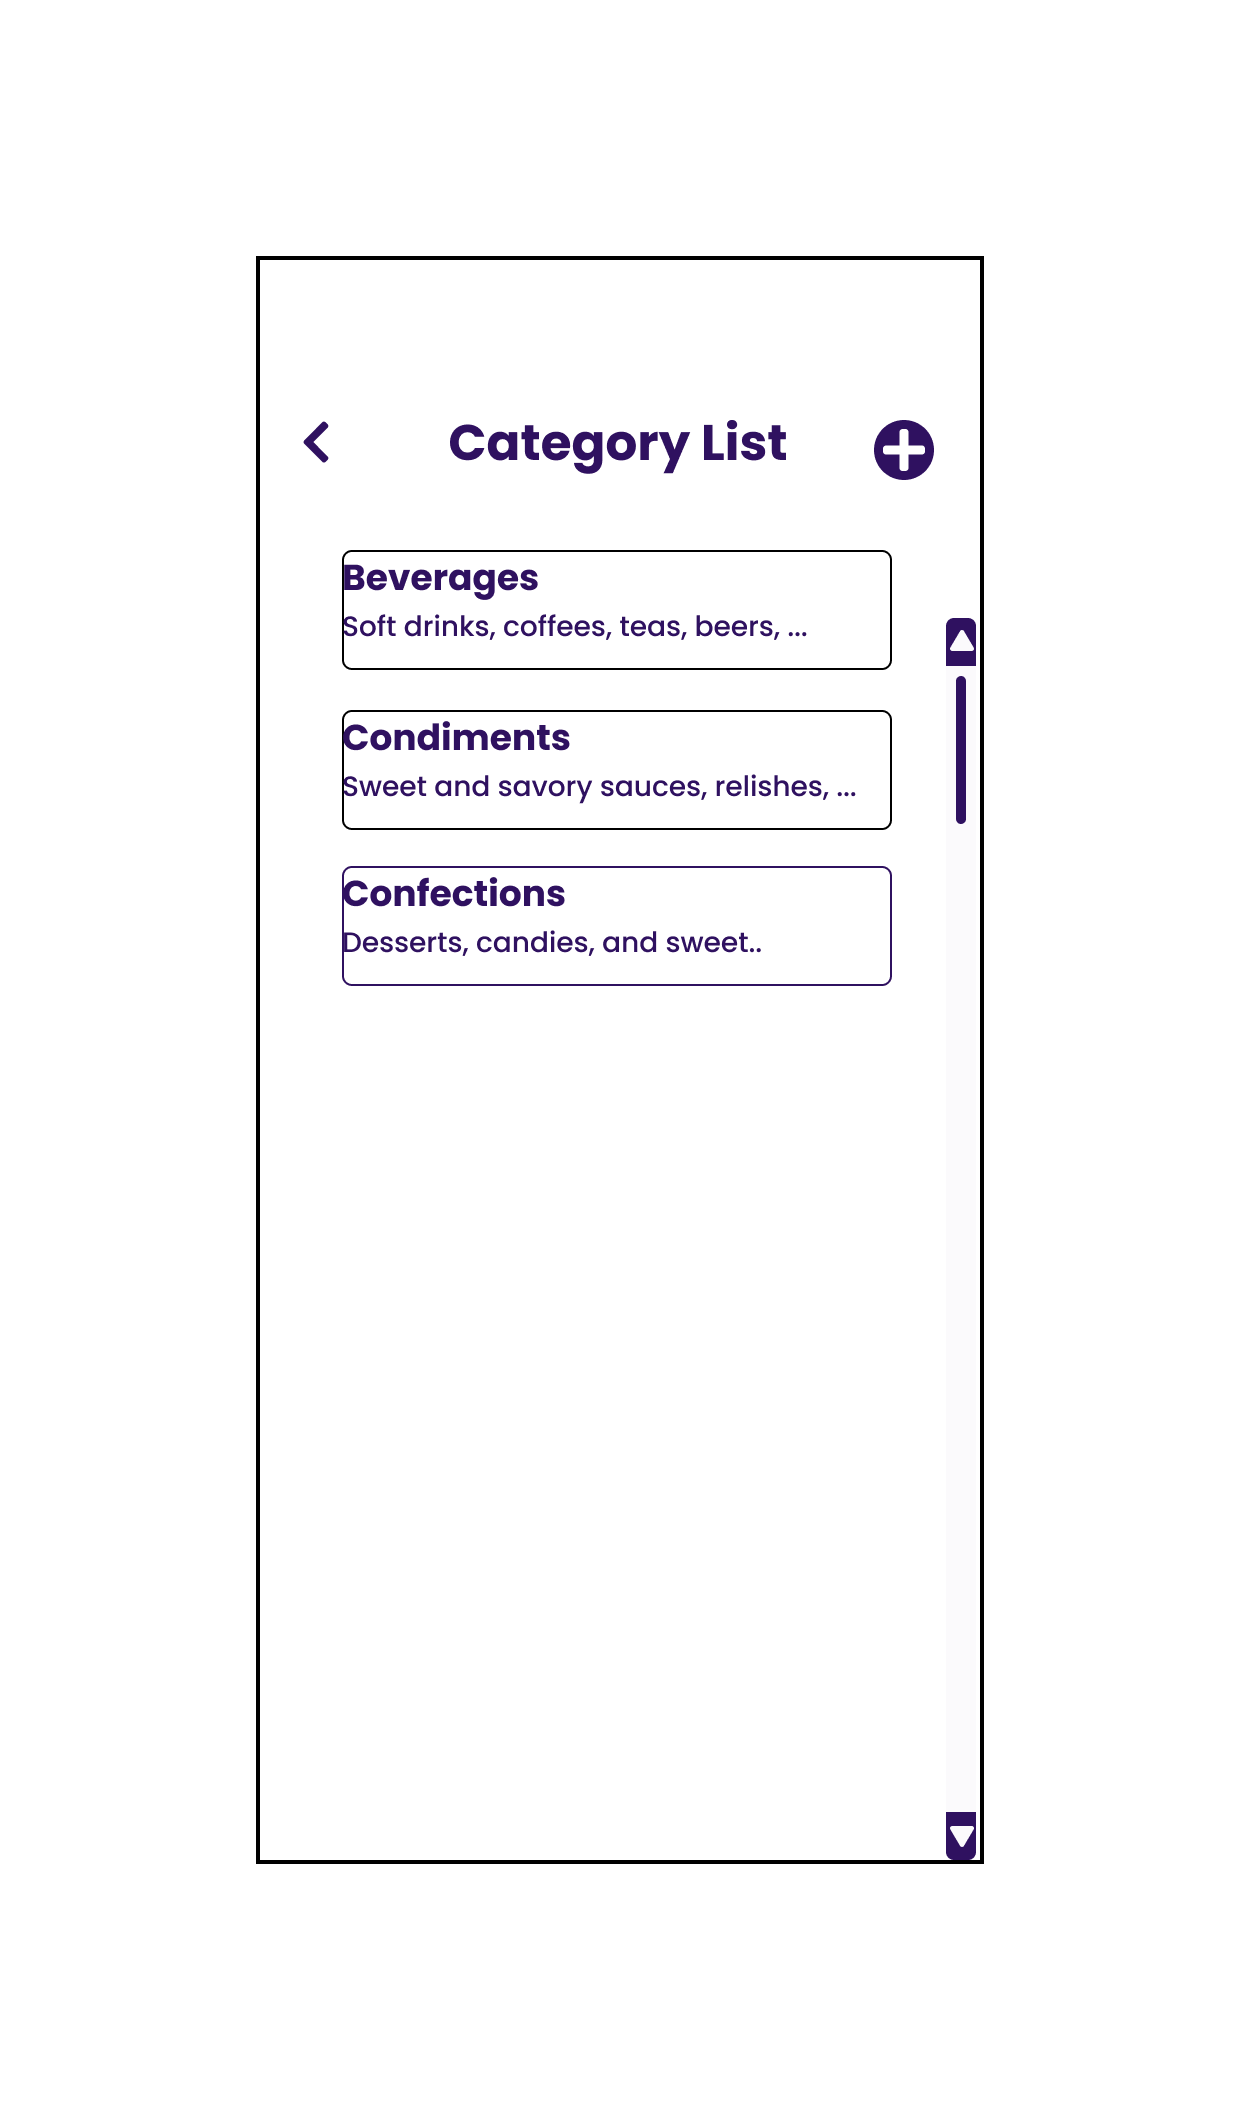
\includegraphics[width=0.57\textwidth]{images/DetailedDesign_Category_List.png}
    \caption{Detail Design: Category List View}
    \label{fig:DetailedDesign_Category_List}
\end{figure}

\begin{figure}[H]
    \centering
    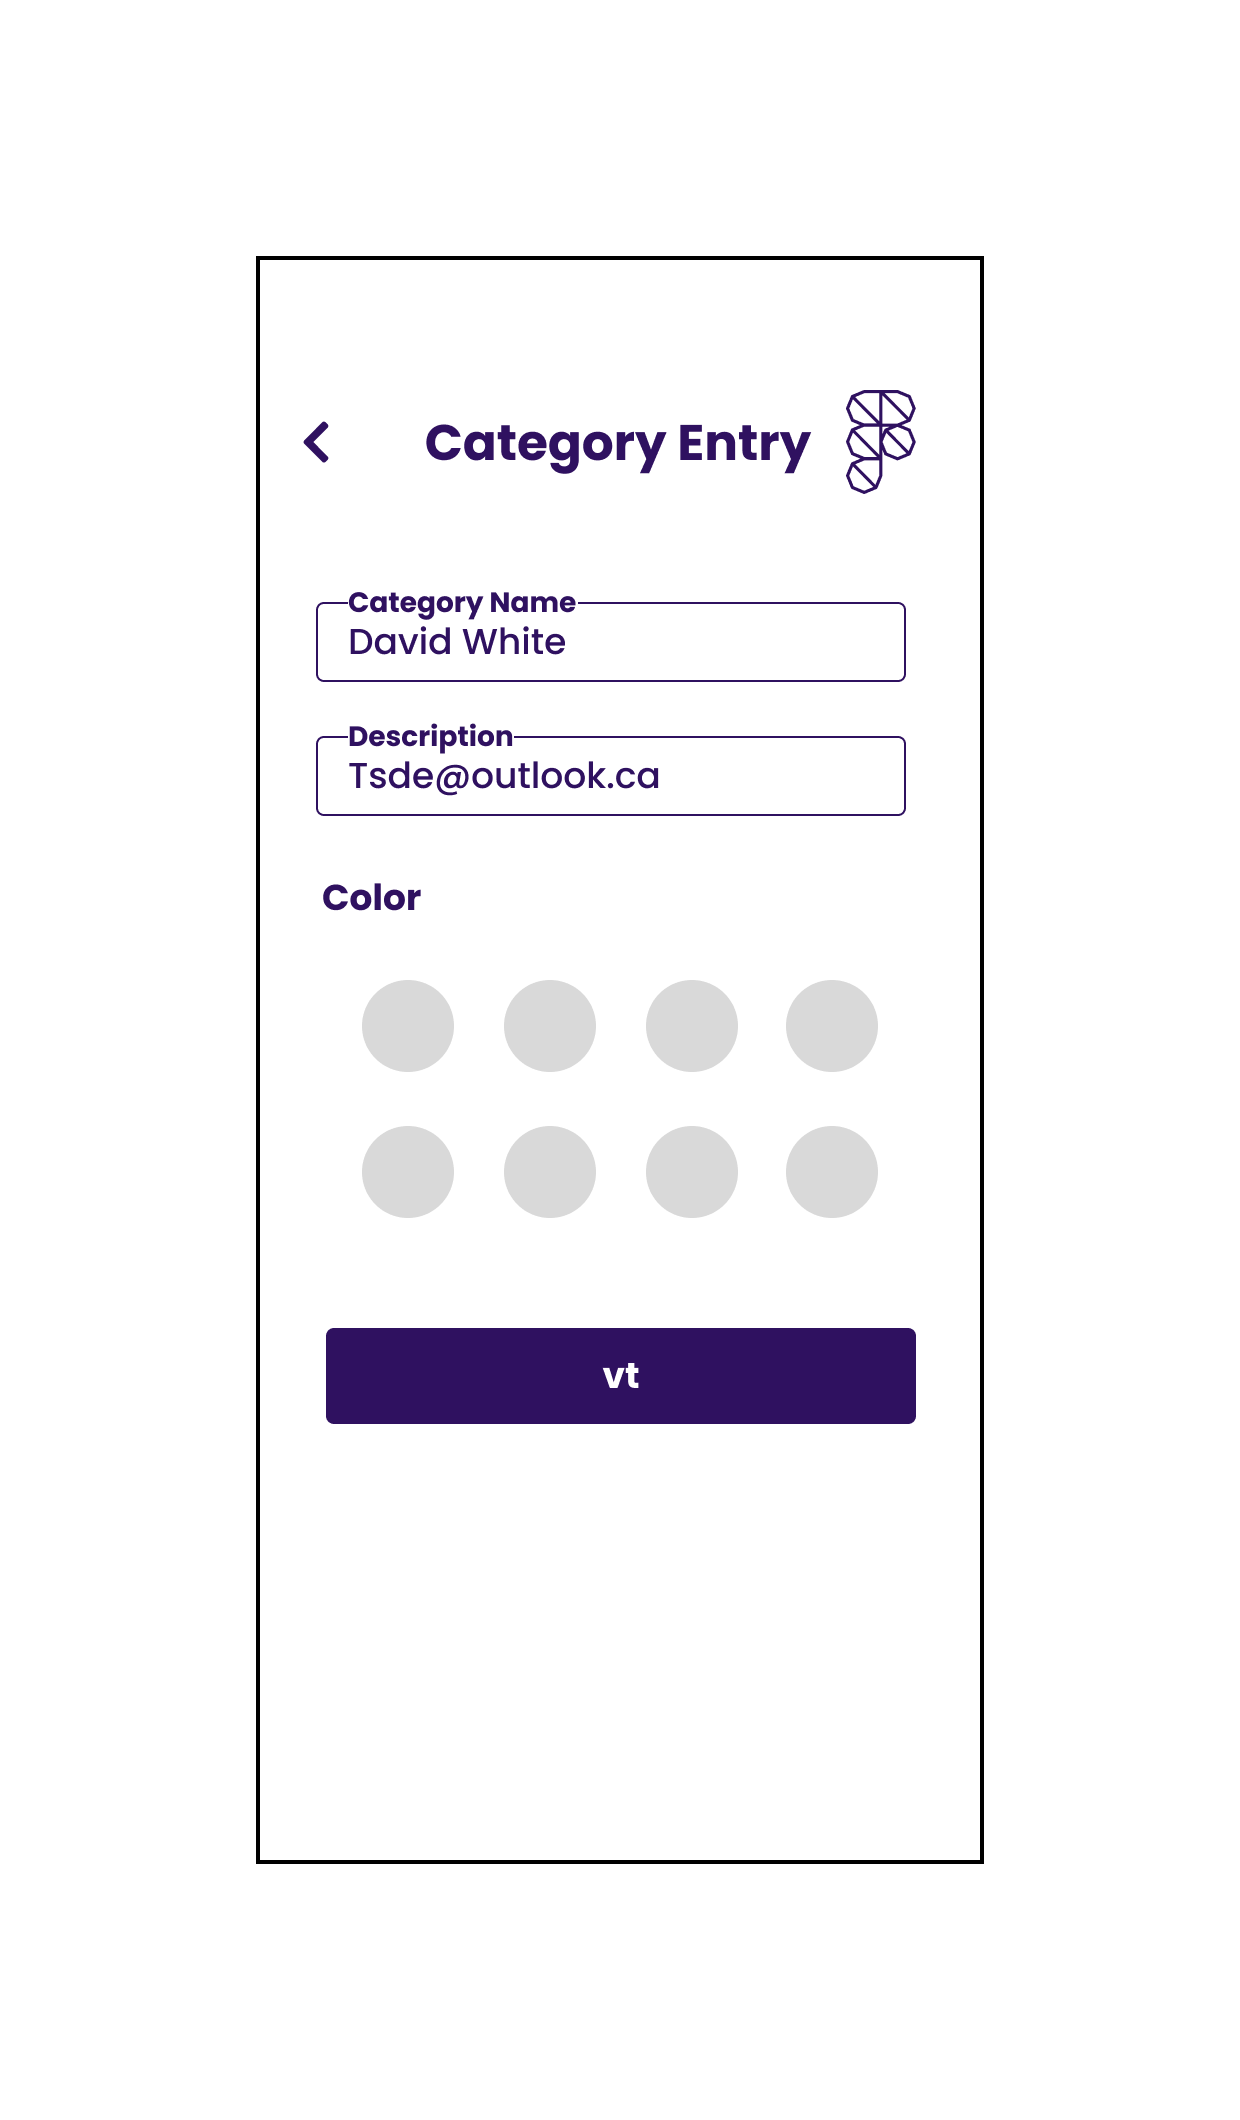
\includegraphics[width=0.57\textwidth]{images/DetailedDesign_Category_Entry.png}
    \caption{Detail Design: Category Entry View}
    \label{fig:DetailedDesign_Category_Entry}
\end{figure}

\subsubsection{Product View}

\begin{figure}[H]
    \centering
    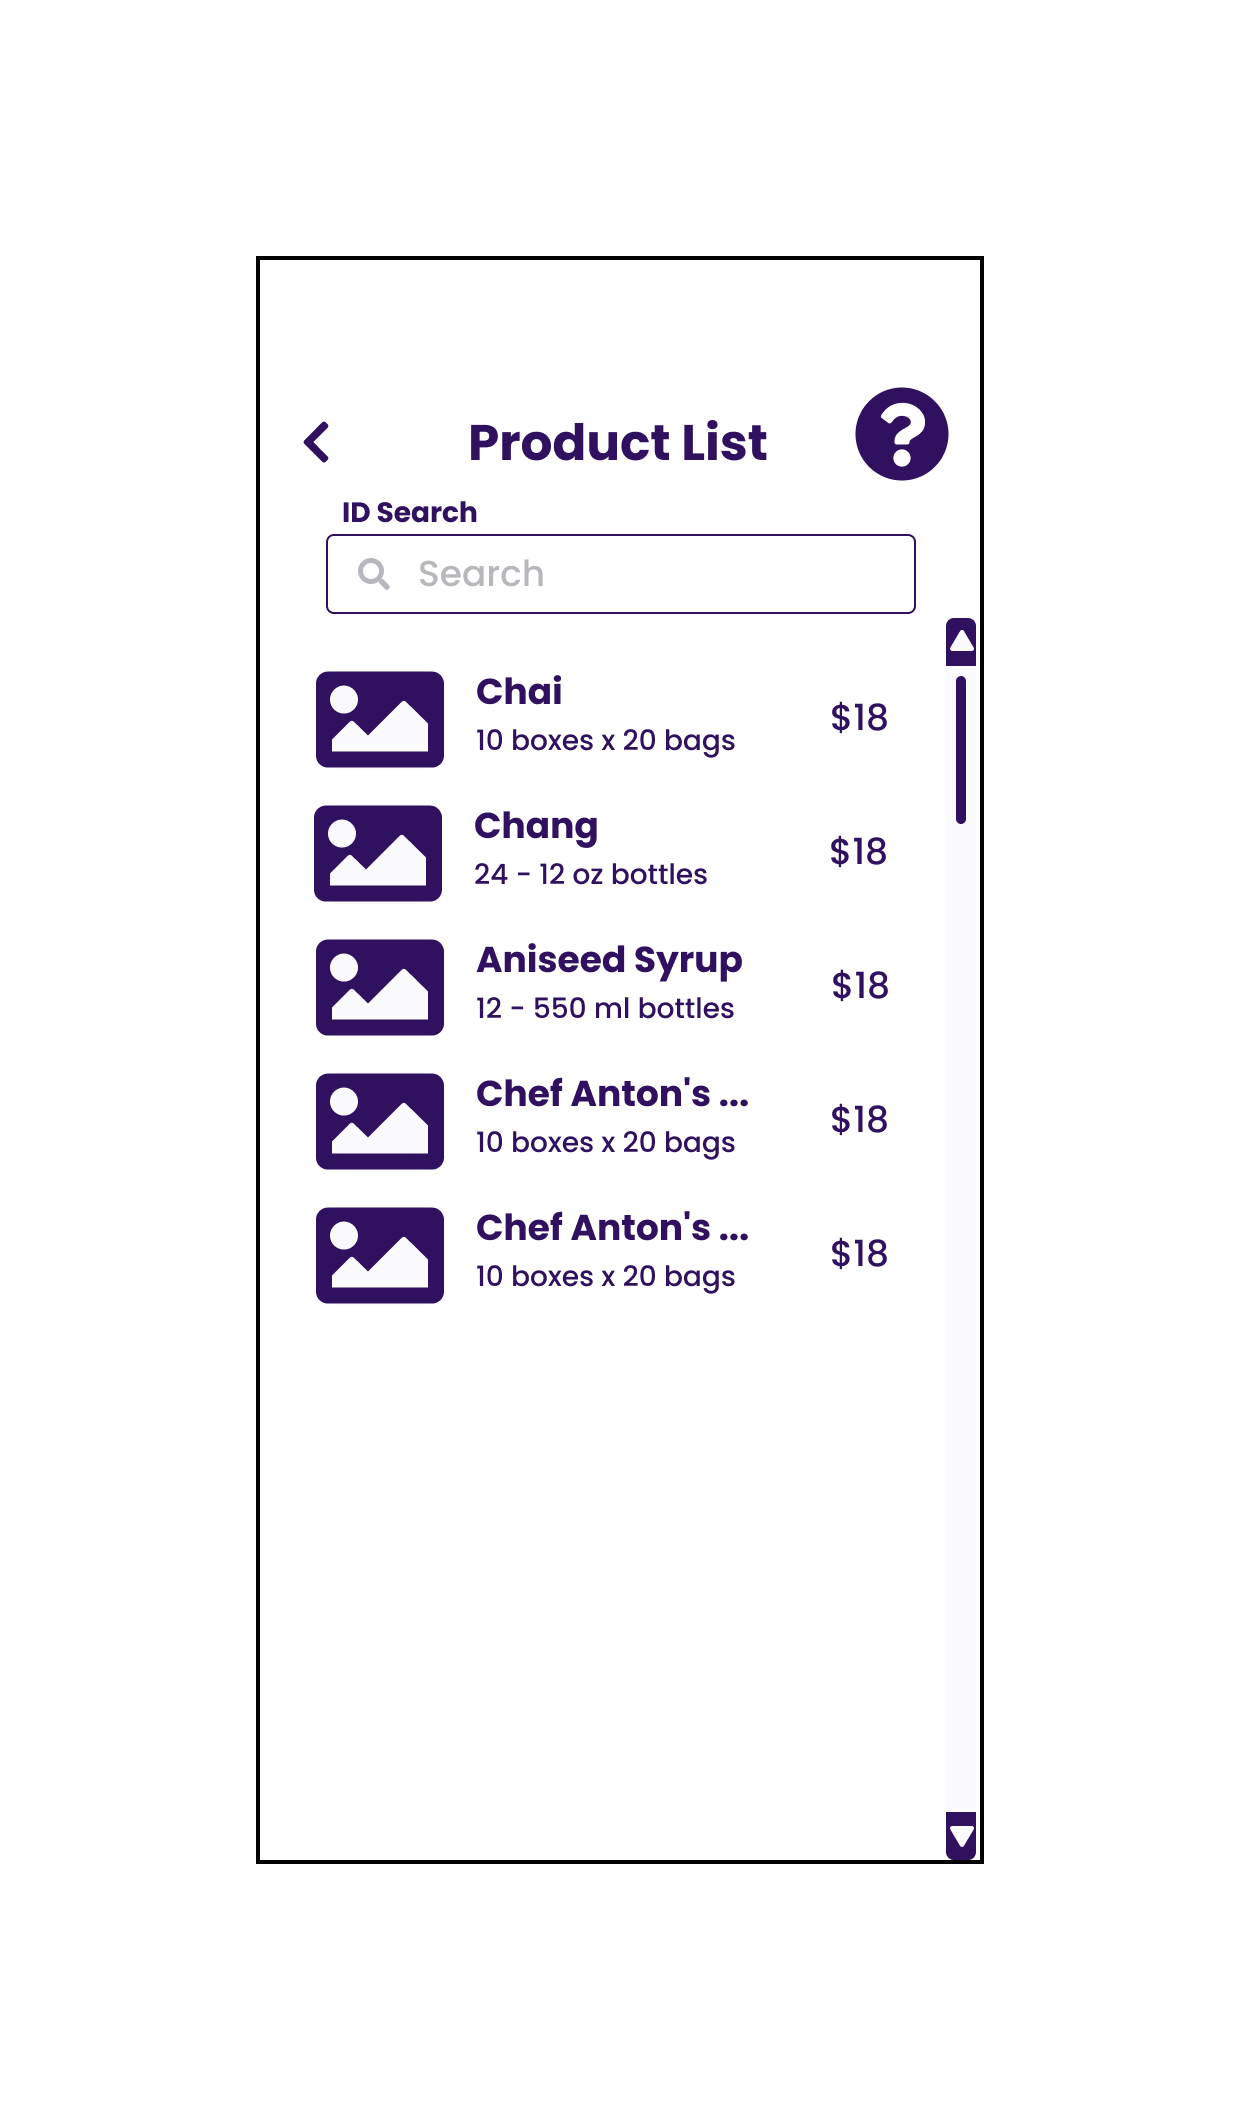
\includegraphics[width=0.57\textwidth]{images/DetailedDesign_Product_List.png}
    \caption{Detail Design: Product List View}
    \label{fig:DetailedDesign_Product_List}
\end{figure}

\begin{figure}[H]
    \centering
    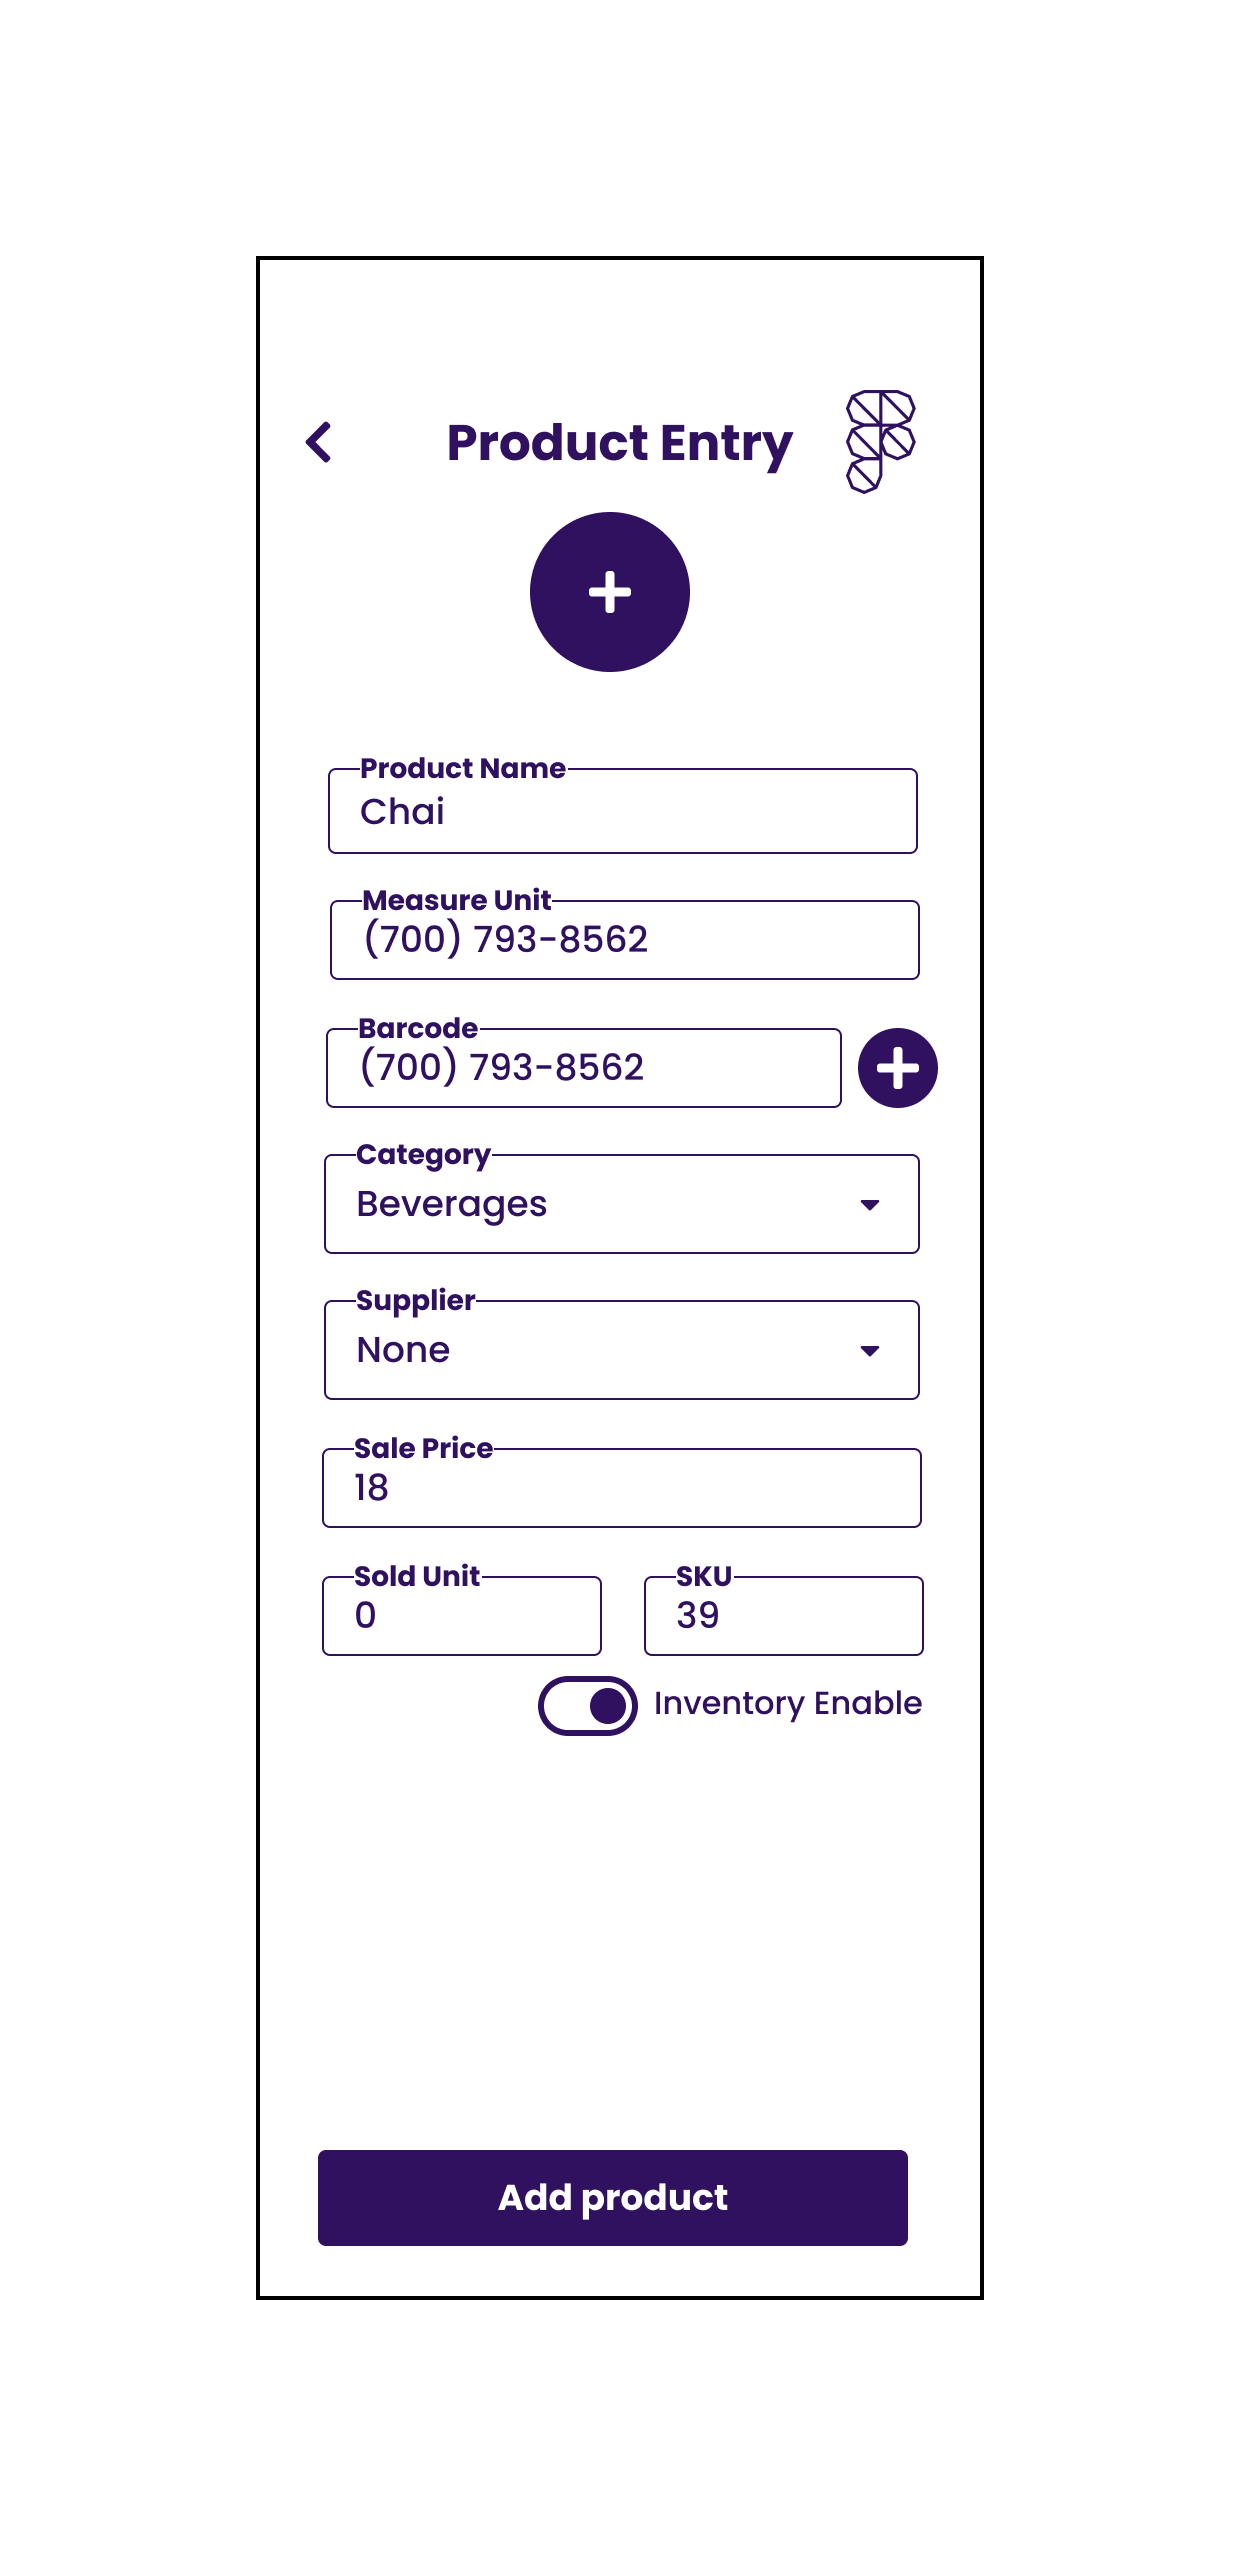
\includegraphics[width=0.57\textwidth]{images/DetailedDesign_Product_Entry.png}
    \caption{Detail Design: Product Entry View}
    \label{fig:DetailedDesign_Product_Entry}
\end{figure}

\subsection{Point of Sales}

\begin{figure}[H]
    \centering
    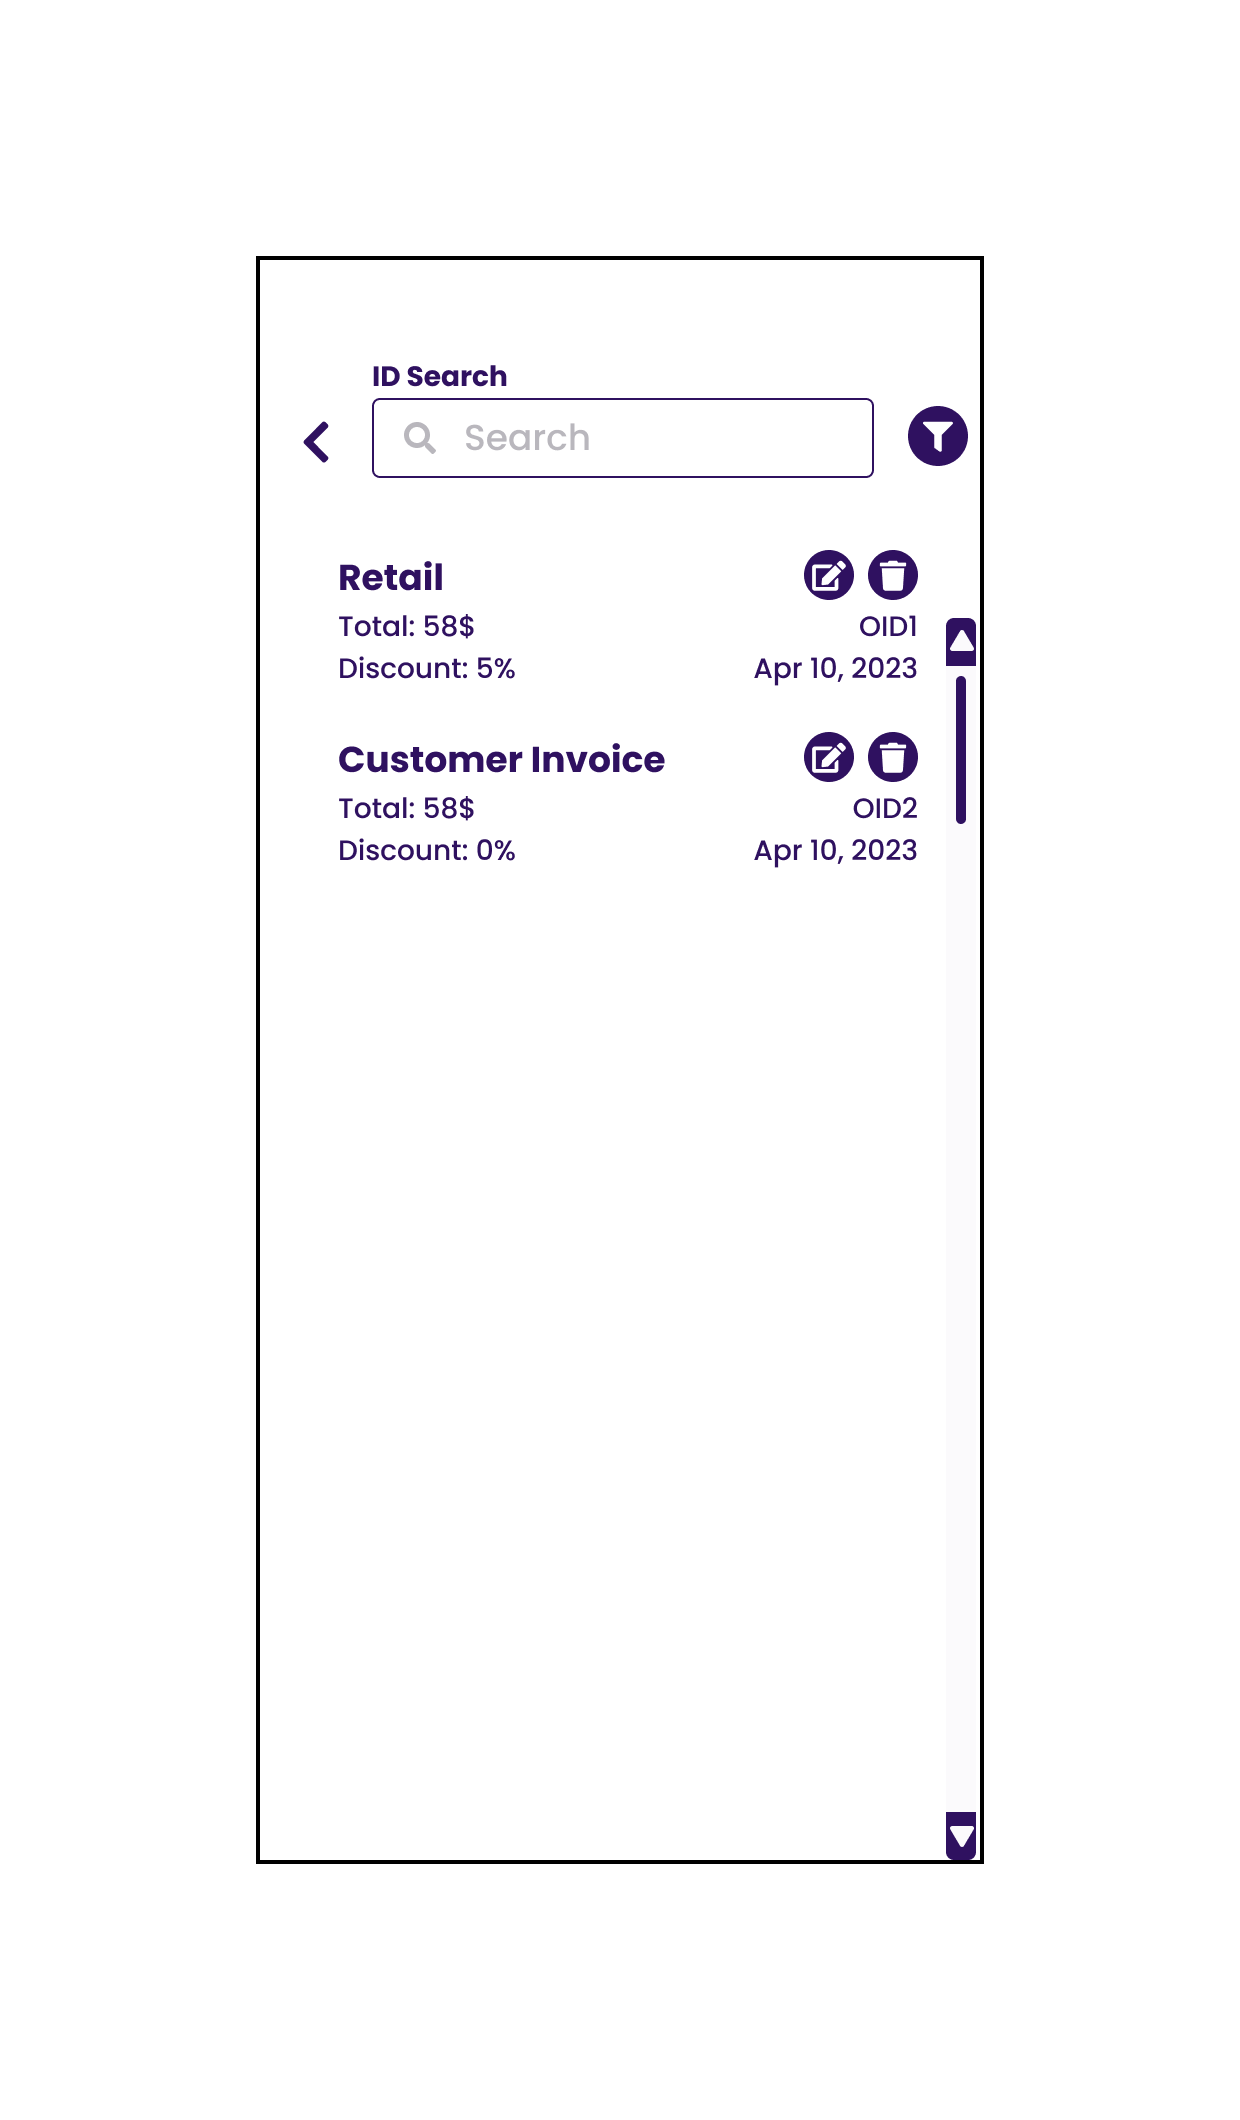
\includegraphics[width=0.57\textwidth]{images/DetailedDesign_Invoice_List.png}
    \caption{Detail Design: Invoice List View}
    \label{fig:DetailedDesign_Invoice_List}
\end{figure}

\begin{figure}[H]
    \centering
    \label{fig:DetailedDesign_Invoice_Entry}

    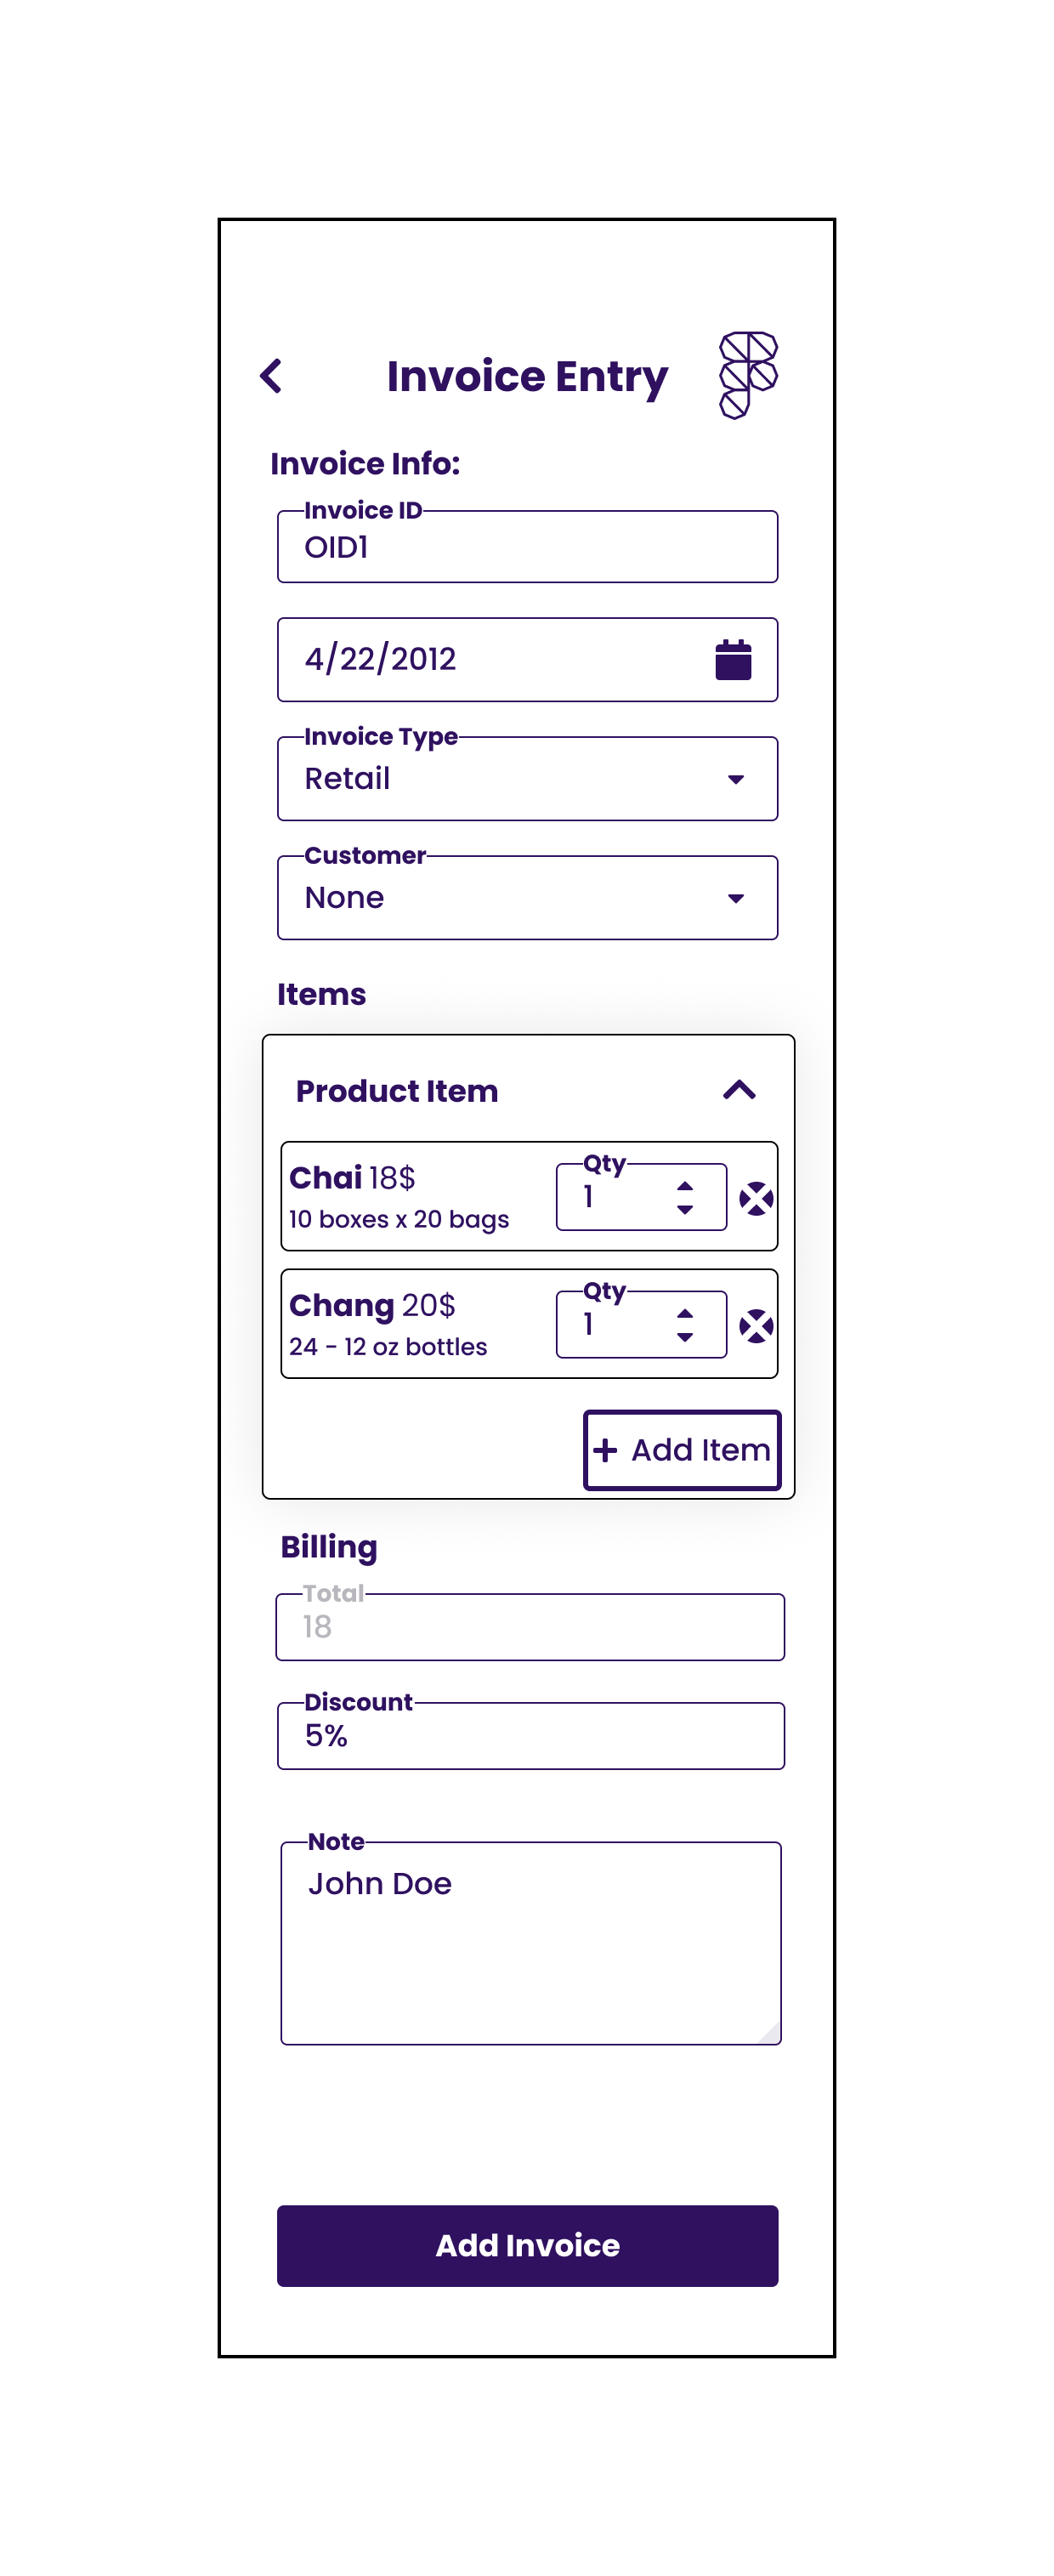
\includegraphics[width=0.60\textwidth]{images/DetailedDesign_Invoice_Entry.png}
    \caption{Detail Design: Invoice Entry View}
\end{figure}


\end{document}